% Options for packages loaded elsewhere
\PassOptionsToPackage{unicode}{hyperref}
\PassOptionsToPackage{hyphens}{url}
\PassOptionsToPackage{dvipsnames,svgnames,x11names}{xcolor}
%
\documentclass[
  letterpaper,
  DIV=11,
  numbers=noendperiod]{scrartcl}

\usepackage{amsmath,amssymb}
\usepackage{iftex}
\ifPDFTeX
  \usepackage[T1]{fontenc}
  \usepackage[utf8]{inputenc}
  \usepackage{textcomp} % provide euro and other symbols
\else % if luatex or xetex
  \usepackage{unicode-math}
  \defaultfontfeatures{Scale=MatchLowercase}
  \defaultfontfeatures[\rmfamily]{Ligatures=TeX,Scale=1}
\fi
\usepackage{lmodern}
\ifPDFTeX\else  
    % xetex/luatex font selection
\fi
% Use upquote if available, for straight quotes in verbatim environments
\IfFileExists{upquote.sty}{\usepackage{upquote}}{}
\IfFileExists{microtype.sty}{% use microtype if available
  \usepackage[]{microtype}
  \UseMicrotypeSet[protrusion]{basicmath} % disable protrusion for tt fonts
}{}
\makeatletter
\@ifundefined{KOMAClassName}{% if non-KOMA class
  \IfFileExists{parskip.sty}{%
    \usepackage{parskip}
  }{% else
    \setlength{\parindent}{0pt}
    \setlength{\parskip}{6pt plus 2pt minus 1pt}}
}{% if KOMA class
  \KOMAoptions{parskip=half}}
\makeatother
\usepackage{xcolor}
\setlength{\emergencystretch}{3em} % prevent overfull lines
\setcounter{secnumdepth}{5}
% Make \paragraph and \subparagraph free-standing
\ifx\paragraph\undefined\else
  \let\oldparagraph\paragraph
  \renewcommand{\paragraph}[1]{\oldparagraph{#1}\mbox{}}
\fi
\ifx\subparagraph\undefined\else
  \let\oldsubparagraph\subparagraph
  \renewcommand{\subparagraph}[1]{\oldsubparagraph{#1}\mbox{}}
\fi

\usepackage{color}
\usepackage{fancyvrb}
\newcommand{\VerbBar}{|}
\newcommand{\VERB}{\Verb[commandchars=\\\{\}]}
\DefineVerbatimEnvironment{Highlighting}{Verbatim}{commandchars=\\\{\}}
% Add ',fontsize=\small' for more characters per line
\usepackage{framed}
\definecolor{shadecolor}{RGB}{241,243,245}
\newenvironment{Shaded}{\begin{snugshade}}{\end{snugshade}}
\newcommand{\AlertTok}[1]{\textcolor[rgb]{0.68,0.00,0.00}{#1}}
\newcommand{\AnnotationTok}[1]{\textcolor[rgb]{0.37,0.37,0.37}{#1}}
\newcommand{\AttributeTok}[1]{\textcolor[rgb]{0.40,0.45,0.13}{#1}}
\newcommand{\BaseNTok}[1]{\textcolor[rgb]{0.68,0.00,0.00}{#1}}
\newcommand{\BuiltInTok}[1]{\textcolor[rgb]{0.00,0.23,0.31}{#1}}
\newcommand{\CharTok}[1]{\textcolor[rgb]{0.13,0.47,0.30}{#1}}
\newcommand{\CommentTok}[1]{\textcolor[rgb]{0.37,0.37,0.37}{#1}}
\newcommand{\CommentVarTok}[1]{\textcolor[rgb]{0.37,0.37,0.37}{\textit{#1}}}
\newcommand{\ConstantTok}[1]{\textcolor[rgb]{0.56,0.35,0.01}{#1}}
\newcommand{\ControlFlowTok}[1]{\textcolor[rgb]{0.00,0.23,0.31}{#1}}
\newcommand{\DataTypeTok}[1]{\textcolor[rgb]{0.68,0.00,0.00}{#1}}
\newcommand{\DecValTok}[1]{\textcolor[rgb]{0.68,0.00,0.00}{#1}}
\newcommand{\DocumentationTok}[1]{\textcolor[rgb]{0.37,0.37,0.37}{\textit{#1}}}
\newcommand{\ErrorTok}[1]{\textcolor[rgb]{0.68,0.00,0.00}{#1}}
\newcommand{\ExtensionTok}[1]{\textcolor[rgb]{0.00,0.23,0.31}{#1}}
\newcommand{\FloatTok}[1]{\textcolor[rgb]{0.68,0.00,0.00}{#1}}
\newcommand{\FunctionTok}[1]{\textcolor[rgb]{0.28,0.35,0.67}{#1}}
\newcommand{\ImportTok}[1]{\textcolor[rgb]{0.00,0.46,0.62}{#1}}
\newcommand{\InformationTok}[1]{\textcolor[rgb]{0.37,0.37,0.37}{#1}}
\newcommand{\KeywordTok}[1]{\textcolor[rgb]{0.00,0.23,0.31}{#1}}
\newcommand{\NormalTok}[1]{\textcolor[rgb]{0.00,0.23,0.31}{#1}}
\newcommand{\OperatorTok}[1]{\textcolor[rgb]{0.37,0.37,0.37}{#1}}
\newcommand{\OtherTok}[1]{\textcolor[rgb]{0.00,0.23,0.31}{#1}}
\newcommand{\PreprocessorTok}[1]{\textcolor[rgb]{0.68,0.00,0.00}{#1}}
\newcommand{\RegionMarkerTok}[1]{\textcolor[rgb]{0.00,0.23,0.31}{#1}}
\newcommand{\SpecialCharTok}[1]{\textcolor[rgb]{0.37,0.37,0.37}{#1}}
\newcommand{\SpecialStringTok}[1]{\textcolor[rgb]{0.13,0.47,0.30}{#1}}
\newcommand{\StringTok}[1]{\textcolor[rgb]{0.13,0.47,0.30}{#1}}
\newcommand{\VariableTok}[1]{\textcolor[rgb]{0.07,0.07,0.07}{#1}}
\newcommand{\VerbatimStringTok}[1]{\textcolor[rgb]{0.13,0.47,0.30}{#1}}
\newcommand{\WarningTok}[1]{\textcolor[rgb]{0.37,0.37,0.37}{\textit{#1}}}

\providecommand{\tightlist}{%
  \setlength{\itemsep}{0pt}\setlength{\parskip}{0pt}}\usepackage{longtable,booktabs,array}
\usepackage{calc} % for calculating minipage widths
% Correct order of tables after \paragraph or \subparagraph
\usepackage{etoolbox}
\makeatletter
\patchcmd\longtable{\par}{\if@noskipsec\mbox{}\fi\par}{}{}
\makeatother
% Allow footnotes in longtable head/foot
\IfFileExists{footnotehyper.sty}{\usepackage{footnotehyper}}{\usepackage{footnote}}
\makesavenoteenv{longtable}
\usepackage{graphicx}
\makeatletter
\def\maxwidth{\ifdim\Gin@nat@width>\linewidth\linewidth\else\Gin@nat@width\fi}
\def\maxheight{\ifdim\Gin@nat@height>\textheight\textheight\else\Gin@nat@height\fi}
\makeatother
% Scale images if necessary, so that they will not overflow the page
% margins by default, and it is still possible to overwrite the defaults
% using explicit options in \includegraphics[width, height, ...]{}
\setkeys{Gin}{width=\maxwidth,height=\maxheight,keepaspectratio}
% Set default figure placement to htbp
\makeatletter
\def\fps@figure{htbp}
\makeatother

\KOMAoption{captions}{tableheading}
\makeatletter
\@ifpackageloaded{caption}{}{\usepackage{caption}}
\AtBeginDocument{%
\ifdefined\contentsname
  \renewcommand*\contentsname{Table of contents}
\else
  \newcommand\contentsname{Table of contents}
\fi
\ifdefined\listfigurename
  \renewcommand*\listfigurename{List of Figures}
\else
  \newcommand\listfigurename{List of Figures}
\fi
\ifdefined\listtablename
  \renewcommand*\listtablename{List of Tables}
\else
  \newcommand\listtablename{List of Tables}
\fi
\ifdefined\figurename
  \renewcommand*\figurename{Figure}
\else
  \newcommand\figurename{Figure}
\fi
\ifdefined\tablename
  \renewcommand*\tablename{Table}
\else
  \newcommand\tablename{Table}
\fi
}
\@ifpackageloaded{float}{}{\usepackage{float}}
\floatstyle{ruled}
\@ifundefined{c@chapter}{\newfloat{codelisting}{h}{lop}}{\newfloat{codelisting}{h}{lop}[chapter]}
\floatname{codelisting}{Stan

Program}
\newcommand*\listoflistings{\listof{codelisting}{List of Listings}}
\makeatother
\makeatletter
\makeatother
\makeatletter
\@ifpackageloaded{caption}{}{\usepackage{caption}}
\@ifpackageloaded{subcaption}{}{\usepackage{subcaption}}
\makeatother
\ifLuaTeX
  \usepackage{selnolig}  % disable illegal ligatures
\fi
\usepackage{bookmark}

\IfFileExists{xurl.sty}{\usepackage{xurl}}{} % add URL line breaks if available
\urlstyle{same} % disable monospaced font for URLs
\hypersetup{
  pdftitle={Churn, Bayes-by, Churn},
  pdfauthor={Michael Betancourt},
  colorlinks=true,
  linkcolor={blue},
  filecolor={Maroon},
  citecolor={Blue},
  urlcolor={Blue},
  pdfcreator={LaTeX via pandoc}}

\title{Churn, Bayes-by, Churn}
\author{Michael Betancourt}
\date{2026-05-01}

\begin{document}
\maketitle
\begin{abstract}
More case studies are available on my
\href{http://www.symplectomorphic.com/writing/\#\#case-studies}{website}.

A repository containing all of the files used to generate this chapter
is available on
\href{https://github.com/betanalpha/quarto_chapters/tree/main/case_studies/churn}{GitHub}.
\end{abstract}

\renewcommand*\contentsname{Table of contents}
{
\hypersetup{linkcolor=}
\setcounter{tocdepth}{3}
\tableofcontents
}
How do customers bring value to a company? In many cases value is driven
not so much by the total number of customers at any given time, but
rather for how long those customers will stay engaged. This constant ebb
and flow of active customers is known as \textbf{churn}.

To properly forecast income for a company in this case, need to infer
when customers will leave. In this case study we'll model the lifetime
of bank customers using survival modeling techniques, and then use those
inferences to predict the most profitable customer segments.

\section{Setup}\label{setup}

Let's begin by setting up our local \texttt{python} environment.

\begin{Shaded}
\begin{Highlighting}[]
\ImportTok{import}\NormalTok{ matplotlib}
\ImportTok{import}\NormalTok{ matplotlib.pyplot }\ImportTok{as}\NormalTok{ plot}
\NormalTok{plot.rcParams[}\StringTok{\textquotesingle{}figure.figsize\textquotesingle{}}\NormalTok{] }\OperatorTok{=}\NormalTok{ [}\DecValTok{8}\NormalTok{, }\DecValTok{4}\NormalTok{]}
\NormalTok{plot.rcParams[}\StringTok{\textquotesingle{}figure.dpi\textquotesingle{}}\NormalTok{] }\OperatorTok{=} \DecValTok{100}
\NormalTok{plot.rcParams[}\StringTok{\textquotesingle{}font.family\textquotesingle{}}\NormalTok{] }\OperatorTok{=} \StringTok{"Serif"}

\ImportTok{import}\NormalTok{ math}
\ImportTok{import}\NormalTok{ numpy}
\ImportTok{import}\NormalTok{ json}
\end{Highlighting}
\end{Shaded}

This includes loading up \texttt{pystan}.

\begin{Shaded}
\begin{Highlighting}[]
\CommentTok{\# Needed to run pystan through a jupyter kernel}
\ImportTok{import}\NormalTok{ nest\_asyncio}
\NormalTok{nest\_asyncio.}\BuiltInTok{apply}\NormalTok{()}

\ImportTok{import}\NormalTok{ stan}
\end{Highlighting}
\end{Shaded}

Next, we have a suite Markov chain Monte Carlo diagnostics and
estimation tools; this code and supporting documentation are both
available on
\href{https://github.com/betanalpha/mcmc_diagnostics}{GitHub}.

\begin{Shaded}
\begin{Highlighting}[]
\ImportTok{import}\NormalTok{ mcmc\_analysis\_tools\_pystan3 }\ImportTok{as}\NormalTok{ util}
\end{Highlighting}
\end{Shaded}

Finally, we have a suite of probabilistic visualization functions based
on Markov chain Monte Carlo estimation. Again the code and supporting
documentation are available on
\href{https://github.com/betanalpha/mcmc_visualization_tools}{GitHub}.

\begin{Shaded}
\begin{Highlighting}[]
\ImportTok{import}\NormalTok{ mcmc\_visualization\_tools }\ImportTok{as}\NormalTok{ putil}
\end{Highlighting}
\end{Shaded}

\section{Data Exploration}\label{data-exploration}

To better understand customer churn, customer acquisition and loss were
recorded across a sixty month observation period. Only those customers
who joined after the observation period were recorded, but many
customers were still active when the observation period ended.

\begin{Shaded}
\begin{Highlighting}[]
\ControlFlowTok{with} \BuiltInTok{open}\NormalTok{(}\StringTok{"data/historical\_data.json"}\NormalTok{, }\StringTok{"r"}\NormalTok{) }\ImportTok{as}\NormalTok{ infile:}
\NormalTok{  data }\OperatorTok{=}\NormalTok{ json.load(infile)}
\end{Highlighting}
\end{Shaded}

All times were recorded in months relative to the start of the
observation window. In this units, the observation period started at
time \(T_{0} = 0 \text{months}\) and ended at time
\(T_{1} = 60 \text{months}\).

\begin{Shaded}
\begin{Highlighting}[]
\BuiltInTok{print}\NormalTok{(}\SpecialStringTok{f\textquotesingle{}Observation period: [}\SpecialCharTok{\{}\NormalTok{data[}\StringTok{\textquotesingle{}T0\textquotesingle{}}\NormalTok{]}\SpecialCharTok{\}}\SpecialStringTok{, }\SpecialCharTok{\{}\NormalTok{data[}\StringTok{\textquotesingle{}T1\textquotesingle{}}\NormalTok{]}\SpecialCharTok{\}}\SpecialStringTok{]\textquotesingle{}}\NormalTok{)}
\end{Highlighting}
\end{Shaded}

\begin{verbatim}
Observation period: [0, 60]
\end{verbatim}

In total, 2243 customers had churned by the end of the observation
period, with 257 additional customers still active.

\begin{Shaded}
\begin{Highlighting}[]
\BuiltInTok{print}\NormalTok{(}\SpecialStringTok{f\textquotesingle{}}\SpecialCharTok{\{}\NormalTok{data[}\StringTok{\textquotesingle{}N\_churn\textquotesingle{}}\NormalTok{]}\SpecialCharTok{\}}\SpecialStringTok{ churned customers\textquotesingle{}}\NormalTok{)}
\end{Highlighting}
\end{Shaded}

\begin{verbatim}
2243 churned customers
\end{verbatim}

\begin{Shaded}
\begin{Highlighting}[]
\BuiltInTok{print}\NormalTok{(}\SpecialStringTok{f\textquotesingle{}}\SpecialCharTok{\{}\NormalTok{data[}\StringTok{\textquotesingle{}N\_active\textquotesingle{}}\NormalTok{]}\SpecialCharTok{\}}\SpecialStringTok{ active customers\textquotesingle{}}\NormalTok{)}
\end{Highlighting}
\end{Shaded}

\begin{verbatim}
257 active customers
\end{verbatim}

The hard cutoff of the observation period results in some interesting
selection effects in the observations. As we reach the end of the
observation period, churned customers are less likely to have joined
because they had less time to leave before the cutoff. On the other
hand, active customers were more likely to join as we approached the
cutoff, where they had less time to leave.

\begin{Shaded}
\begin{Highlighting}[]
\NormalTok{putil.plot\_line\_hists(plot.gca(),}
\NormalTok{                      data[}\StringTok{\textquotesingle{}t\_join\_churn\textquotesingle{}}\NormalTok{],}
\NormalTok{                      data[}\StringTok{\textquotesingle{}t\_join\_active\textquotesingle{}}\NormalTok{],}
\NormalTok{                      data[}\StringTok{\textquotesingle{}T0\textquotesingle{}}\NormalTok{] }\OperatorTok{{-}} \DecValTok{3}\NormalTok{, data[}\StringTok{\textquotesingle{}T1\textquotesingle{}}\NormalTok{] }\OperatorTok{+} \DecValTok{3}\NormalTok{, }\DecValTok{3}\NormalTok{,}
\NormalTok{                      xlabel}\OperatorTok{=}\StringTok{"Time Customer Joins (months)"}\NormalTok{)}

\NormalTok{plot.gca().axvline(x}\OperatorTok{=}\NormalTok{data[}\StringTok{\textquotesingle{}T0\textquotesingle{}}\NormalTok{], linewidth}\OperatorTok{=}\DecValTok{2}\NormalTok{,}
\NormalTok{                   linestyle}\OperatorTok{=}\StringTok{\textquotesingle{}dashed\textquotesingle{}}\NormalTok{, color}\OperatorTok{=}\StringTok{"\#DDDDDD"}\NormalTok{)}
\NormalTok{plot.gca().axvline(x}\OperatorTok{=}\NormalTok{data[}\StringTok{\textquotesingle{}T1\textquotesingle{}}\NormalTok{], linewidth}\OperatorTok{=}\DecValTok{2}\NormalTok{,}
\NormalTok{                   linestyle}\OperatorTok{=}\StringTok{\textquotesingle{}dashed\textquotesingle{}}\NormalTok{, color}\OperatorTok{=}\StringTok{"\#DDDDDD"}\NormalTok{)}

\NormalTok{plot.gca().text(}\DecValTok{10}\NormalTok{, }\DecValTok{80}\NormalTok{, }\StringTok{"Churned}\CharTok{\textbackslash{}n}\StringTok{Customers"}\NormalTok{,}
\NormalTok{                color}\OperatorTok{=}\StringTok{\textquotesingle{}black\textquotesingle{}}\NormalTok{)}

\NormalTok{plot.gca().text(}\DecValTok{35}\NormalTok{, }\DecValTok{25}\NormalTok{, }\StringTok{"Active}\CharTok{\textbackslash{}n}\StringTok{Customers"}\NormalTok{,}
\NormalTok{                color}\OperatorTok{=}\NormalTok{putil.mid\_teal)}

\NormalTok{plot.show()}
\end{Highlighting}
\end{Shaded}

\includegraphics{churn_files/figure-pdf/cell-10-output-1.png}

Because data collection ended at \(T_{1}\), we observed leave times for
only the customers who had churned before the observational period
ended.

\begin{Shaded}
\begin{Highlighting}[]
\NormalTok{putil.plot\_line\_hist(plot.gca(), data[}\StringTok{\textquotesingle{}t\_leave\_churn\textquotesingle{}}\NormalTok{],}
\NormalTok{                     data[}\StringTok{\textquotesingle{}T0\textquotesingle{}}\NormalTok{] }\OperatorTok{{-}} \DecValTok{3}\NormalTok{, data[}\StringTok{\textquotesingle{}T1\textquotesingle{}}\NormalTok{] }\OperatorTok{+} \DecValTok{3}\NormalTok{, }\DecValTok{3}\NormalTok{,}
\NormalTok{                     xlabel}\OperatorTok{=}\StringTok{"Time Customer Leaves (months)"}\NormalTok{)}

\NormalTok{plot.gca().axvline(x}\OperatorTok{=}\NormalTok{data[}\StringTok{\textquotesingle{}T0\textquotesingle{}}\NormalTok{], linewidth}\OperatorTok{=}\DecValTok{2}\NormalTok{,}
\NormalTok{                   linestyle}\OperatorTok{=}\StringTok{\textquotesingle{}dashed\textquotesingle{}}\NormalTok{, color}\OperatorTok{=}\StringTok{"\#DDDDDD"}\NormalTok{)}
\NormalTok{plot.gca().axvline(x}\OperatorTok{=}\NormalTok{data[}\StringTok{\textquotesingle{}T1\textquotesingle{}}\NormalTok{], linewidth}\OperatorTok{=}\DecValTok{2}\NormalTok{,}
\NormalTok{                   linestyle}\OperatorTok{=}\StringTok{\textquotesingle{}dashed\textquotesingle{}}\NormalTok{, color}\OperatorTok{=}\StringTok{"\#DDDDDD"}\NormalTok{)}

\NormalTok{plot.show()}
\end{Highlighting}
\end{Shaded}

\includegraphics{churn_files/figure-pdf/cell-11-output-1.png}

The join and leave times for a particular customer are not as
interesting as their difference, which defines the observed customer
\emph{lifetime} or \emph{tenure} (Figure~\ref{fig-events}).

\begin{figure}

\begin{minipage}{0.05\linewidth}
~\end{minipage}%
%
\begin{minipage}{0.45\linewidth}

\centering{

\captionsetup{labelsep=none}
\includegraphics{figures/events/churn/event.pdf}

}

\subcaption{\label{fig-churn-cust}}

\end{minipage}%
%
\begin{minipage}{0.45\linewidth}

\centering{

\captionsetup{labelsep=none}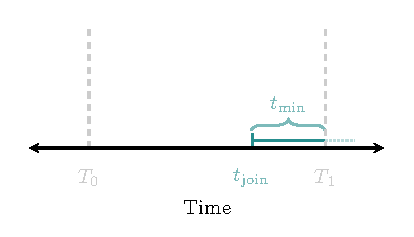
\includegraphics{figures/events/active/event.pdf}

}

\subcaption{\label{fig-active-cust}}

\end{minipage}%
%
\begin{minipage}{0.05\linewidth}
~\end{minipage}%

\caption{\label{fig-events}Our data contains two types of customers (a)
Churned customers joined and then left before the end of the observation
period \([T_{0}, T_{1}]\). Customer lifetime is given by the time
between joining and leaving. (b) Active customers joined during the
observation period, but had not yet left when the observation period
ended. We don't know what the overall tenure for these customers was,
but we can bound it below by \(t_{\min} = T_{1} - t_{\text{join}}\).}

\end{figure}%

While most customers churned after twenty months or so, some more loyal
customers persisted for quite a bit longer.

\begin{Shaded}
\begin{Highlighting}[]
\NormalTok{tenure\_churn }\OperatorTok{=}\NormalTok{ [ tl }\OperatorTok{{-}}\NormalTok{ tj }\ControlFlowTok{for}\NormalTok{ tj, tl}
                 \KeywordTok{in} \BuiltInTok{zip}\NormalTok{(data[}\StringTok{\textquotesingle{}t\_join\_churn\textquotesingle{}}\NormalTok{],}
\NormalTok{                        data[}\StringTok{\textquotesingle{}t\_leave\_churn\textquotesingle{}}\NormalTok{]) ]}

\NormalTok{putil.plot\_line\_hist(plot.gca(), tenure\_churn,}
\NormalTok{                     data[}\StringTok{\textquotesingle{}T0\textquotesingle{}}\NormalTok{] }\OperatorTok{{-}} \DecValTok{2}\NormalTok{, data[}\StringTok{\textquotesingle{}T1\textquotesingle{}}\NormalTok{] }\OperatorTok{+} \DecValTok{2}\NormalTok{, }\DecValTok{2}\NormalTok{,}
\NormalTok{                     xlabel}\OperatorTok{=}\StringTok{"Customer Tenure (months)"}\NormalTok{)}
\NormalTok{plot.show()}
\end{Highlighting}
\end{Shaded}

\includegraphics{churn_files/figure-pdf/cell-12-output-1.png}

The data also includes demographic information for each of the observed
customers, regardless of whether or not they had left by the end of the
observation period (\textbf{Table 1}).

A little over half of all churned customers participated in online
banking.

\begin{Shaded}
\begin{Highlighting}[]
\NormalTok{N\_online\_banking }\OperatorTok{=} \BuiltInTok{sum}\NormalTok{([ }\DecValTok{1} \ControlFlowTok{for}\NormalTok{ o }\KeywordTok{in}
\NormalTok{                         data[}\StringTok{\textquotesingle{}online\_banking\_churn\textquotesingle{}}\NormalTok{]}
                         \ControlFlowTok{if}\NormalTok{ o }\OperatorTok{==} \DecValTok{1}\NormalTok{ ])}

\BuiltInTok{print}\NormalTok{(}\SpecialStringTok{f\textquotesingle{}}\SpecialCharTok{\{}\NormalTok{N\_online\_banking}\SpecialCharTok{\}}\SpecialStringTok{ out of }\SpecialCharTok{\{}\NormalTok{data[}\StringTok{\textquotesingle{}N\_churn\textquotesingle{}}\NormalTok{]}\SpecialCharTok{\}}\SpecialStringTok{ \textquotesingle{}}
      \SpecialStringTok{f\textquotesingle{}(}\SpecialCharTok{\{}\DecValTok{100} \OperatorTok{*}\NormalTok{ N\_online\_banking }\OperatorTok{/}\NormalTok{ data[}\StringTok{\textquotesingle{}N\_churn\textquotesingle{}}\NormalTok{]}\SpecialCharTok{:.2f\}}\SpecialStringTok{\%) \textquotesingle{}}
       \StringTok{\textquotesingle{}churned customers used online banking.\textquotesingle{}}\NormalTok{)}
\end{Highlighting}
\end{Shaded}

\begin{verbatim}
1548 out of 2243 (69.01%) churned customers used online banking.
\end{verbatim}

The other demographic variables span a pretty wide range of values, but
there is some interesting structure. For example, we can see a secondary
peak of high wealth, high margin customers.

\begin{Shaded}
\begin{Highlighting}[]
\NormalTok{bin\_min }\OperatorTok{=}\NormalTok{ [ }\DecValTok{0}\NormalTok{, }\DecValTok{0}\NormalTok{, }\DecValTok{0}\NormalTok{, }\DecValTok{0}\NormalTok{ ]}
\NormalTok{bin\_max }\OperatorTok{=}\NormalTok{ [ }\DecValTok{100}\NormalTok{, }\DecValTok{15}\NormalTok{, }\FloatTok{1.05}\NormalTok{, }\DecValTok{1000}\NormalTok{ ]}
\NormalTok{bin\_delta }\OperatorTok{=}\NormalTok{ [ }\DecValTok{5}\NormalTok{, }\DecValTok{1}\NormalTok{, }\FloatTok{0.05}\NormalTok{, }\DecValTok{10}\NormalTok{ ]}

\NormalTok{f, axarr }\OperatorTok{=}\NormalTok{ plot.subplots(}\DecValTok{2}\NormalTok{, }\DecValTok{2}\NormalTok{, layout}\OperatorTok{=}\StringTok{"constrained"}\NormalTok{)}

\ControlFlowTok{for}\NormalTok{ i }\KeywordTok{in} \BuiltInTok{range}\NormalTok{(data[}\StringTok{\textquotesingle{}I\textquotesingle{}}\NormalTok{]):}
\NormalTok{  i1 }\OperatorTok{=}\NormalTok{ i }\OperatorTok{//} \DecValTok{2}
\NormalTok{  i2 }\OperatorTok{=}\NormalTok{ i }\OperatorTok{\%} \DecValTok{2}

\NormalTok{  putil.plot\_line\_hist(axarr[i1, i2],}
\NormalTok{                       [ x[i] }\ControlFlowTok{for}\NormalTok{ x }\KeywordTok{in}\NormalTok{ data[}\StringTok{\textquotesingle{}X\_churn\textquotesingle{}}\NormalTok{] ],}
\NormalTok{                       bin\_min[i], bin\_max[i], bin\_delta[i],}
\NormalTok{                       xlabel}\OperatorTok{=}\NormalTok{data[}\StringTok{\textquotesingle{}x\_names\textquotesingle{}}\NormalTok{][i])}

\NormalTok{plot.show()}
\end{Highlighting}
\end{Shaded}

\begin{verbatim}
1 values (0.04%) fell below the histogram binning.
6 values (0.27%) fell above the histogram binning.
\end{verbatim}

\includegraphics{churn_files/figure-pdf/cell-14-output-2.png}

Given this demographic information, a natural question to consider is
whether or not any behavior of interest, such as customer lifetimes,
varies across the demographics. The empirical covariation doesn't show
any obvious pattern.

\begin{Shaded}
\begin{Highlighting}[]
\NormalTok{putil.plot\_line\_hists(plot.gca(),}
\NormalTok{                      [ t }\ControlFlowTok{for}\NormalTok{ t, o}
                        \KeywordTok{in} \BuiltInTok{zip}\NormalTok{(tenure\_churn,}
\NormalTok{                               data[}\StringTok{\textquotesingle{}online\_banking\_churn\textquotesingle{}}\NormalTok{])}
                        \ControlFlowTok{if}\NormalTok{ o }\OperatorTok{==} \DecValTok{0}\NormalTok{ ],}
\NormalTok{                      [ t }\ControlFlowTok{for}\NormalTok{ t, o}
                        \KeywordTok{in} \BuiltInTok{zip}\NormalTok{(tenure\_churn,}
\NormalTok{                               data[}\StringTok{\textquotesingle{}online\_banking\_churn\textquotesingle{}}\NormalTok{])}
                        \ControlFlowTok{if}\NormalTok{ o }\OperatorTok{==} \DecValTok{1}\NormalTok{ ],}
\NormalTok{                      data[}\StringTok{\textquotesingle{}T0\textquotesingle{}}\NormalTok{] }\OperatorTok{{-}} \DecValTok{2}\NormalTok{, data[}\StringTok{\textquotesingle{}T1\textquotesingle{}}\NormalTok{] }\OperatorTok{+} \DecValTok{2}\NormalTok{, }\DecValTok{2}\NormalTok{,}
\NormalTok{                      prob}\OperatorTok{=}\VariableTok{True}\NormalTok{,}
\NormalTok{                      xlabel}\OperatorTok{=}\StringTok{"Customer Tenure (months)"}\NormalTok{)}

\NormalTok{plot.gca().text(}\DecValTok{15}\NormalTok{, }\FloatTok{0.04}\NormalTok{, }\StringTok{"No Online Banking"}\NormalTok{,}
\NormalTok{                color}\OperatorTok{=}\StringTok{\textquotesingle{}black\textquotesingle{}}\NormalTok{)}

\NormalTok{plot.gca().text(}\DecValTok{10}\NormalTok{, }\FloatTok{0.12}\NormalTok{, }\StringTok{"Online Banking"}\NormalTok{,}
\NormalTok{                color}\OperatorTok{=}\NormalTok{putil.mid\_teal)}

\NormalTok{plot.show()}
\end{Highlighting}
\end{Shaded}

\includegraphics{churn_files/figure-pdf/cell-15-output-1.png}

\begin{Shaded}
\begin{Highlighting}[]
\NormalTok{f, axarr }\OperatorTok{=}\NormalTok{ plot.subplots(}\DecValTok{2}\NormalTok{, }\DecValTok{2}\NormalTok{, layout}\OperatorTok{=}\StringTok{"constrained"}\NormalTok{)}

\ControlFlowTok{for}\NormalTok{ i }\KeywordTok{in} \BuiltInTok{range}\NormalTok{(data[}\StringTok{\textquotesingle{}I\textquotesingle{}}\NormalTok{]):}
\NormalTok{  i1 }\OperatorTok{=}\NormalTok{ i }\OperatorTok{//} \DecValTok{2}
\NormalTok{  i2 }\OperatorTok{=}\NormalTok{ i }\OperatorTok{\%} \DecValTok{2}

\NormalTok{  axarr[i1, i2].scatter([ x[i] }\ControlFlowTok{for}\NormalTok{ x }\KeywordTok{in}\NormalTok{ data[}\StringTok{\textquotesingle{}X\_churn\textquotesingle{}}\NormalTok{] ],}
\NormalTok{                        tenure\_churn,}
\NormalTok{                        color}\OperatorTok{=}\StringTok{"black"}\NormalTok{, s}\OperatorTok{=}\DecValTok{2}\NormalTok{)}
\NormalTok{  axarr[i1, i2].set\_xlim([bin\_min[i], bin\_max[i]])}
\NormalTok{  axarr[i1, i2].set\_xlabel(data[}\StringTok{\textquotesingle{}x\_names\textquotesingle{}}\NormalTok{][i])}
\NormalTok{  axarr[i1, i2].set\_ylim([data[}\StringTok{\textquotesingle{}T0\textquotesingle{}}\NormalTok{], data[}\StringTok{\textquotesingle{}T1\textquotesingle{}}\NormalTok{]])}
\NormalTok{  axarr[i1, i2].set\_ylabel(}\StringTok{"Tenure (months)"}\NormalTok{)}

\NormalTok{plot.show()}
\end{Highlighting}
\end{Shaded}

\includegraphics{churn_files/figure-pdf/cell-16-output-1.png}

That said, raw scatter plots are not the most sensitive way to quantify
demographic heterogeneity!

\section{Model 1: Constant Stimulus
Model}\label{model-1-constant-stimulus-model}

Having familiarized ourselves with the data, let's now attempt to infer
the configuration of a customer lifetime model with those observations.

\subsection{Observational Model}\label{observational-model}

Churn is unavoidable in practice; it's only a matter of time before a
customer eventually leaves. Modeling how long it takes for an inevitable
event to occur is the purview of
\href{http://www.symplectomorphic.com/assets/case_studies/survival_modeling.html}{survival
modeling}.

In survival modeling, we don't directly model event times. Instead, we
model the temporal \textbf{stimulus}, classically referred to as the
\textbf{hazard}, that eventually triggers an event to occur. When
considering customer lifetimes, the stimulus might be interpreted as
modeling the overall satisfaction of a customer relative to their other
banking options.

Given a stimulus function \(\lambda(t)\), we can derive a cumulative
stimulus function, \[
\Lambda(t) = \int_{0}^{t} \mathrm{d} t' \, \lambda(t'),
\] which quantifies how much stimulus has built-up by a certain time.
The cumulative stimulus function then defines a complementary cumulative
distribution function, or survival function, \[
S(t)
=
\exp \left( - \Lambda(t) \right).
\] If stimulus accumulates quickly, then the probability that an event
has not yet occurred by a given time rapidly decays.

Finally, given a survival function we can derive a time-to-event model,
\[
p(t) = \lambda(t) \, S(t).
\] Events are most likely to occur when the instantaneous stimulus is
large, but the survival function has not yet decayed too much.

Let's start simple and assume that the stimulus for customer churn is
fixed in time, \[
\lambda(t) = \gamma.
\] In this case, the cumulative stimulus function grows linearly, \[
\Lambda(t)
=
\int_{0}^{t} \mathrm{d} t' \, \lambda(t')
=
\gamma \, t,
\] while the survival function decays exponentially, \[
S(t)
=
\exp \left( - \Lambda(t) \right)
=
\exp(-\gamma \, t).
\]

Conveniently, the resulting time-to-event model reduces to an
exponential probability density function, \begin{align*}
p(t)
&=
\lambda(t) \, S(t)
\\
&=
\gamma \, \exp(-\gamma \, t)
\\
&= \mathrm{exponential}(t \mid \gamma).
\end{align*} This familiar form makes implementing the model in practice
particularly straightforward.

Note that the time-to-event model doesn't model customer leave times but
rather customer tenures, \[
t = t_{\text{leave}} - t_{\text{join}}.
\] In terms of our raw data, the time-to-event model is given by \[
p( t_{\text{leave}} - t_{\text{join}} )
=
\mathrm{exponential}(
  t_{\text{leave}} - t_{\text{join}} \mid \gamma
).
\]

\subsection{Prior Model}\label{prior-model}

To perform a Bayesian analysis, we need to complement this observational
model with a
\href{http://www.symplectomorphic.com/assets/case_studies/prior_modeling.html}{prior
model}. The prior model quantifies any available domain expertise that
we want to incorporate into the analysis.

For this analysis, let's say that our domain expertise was already used
to design the original observation period. Customer tenure longer than
60 months is not impossible, but it should be relatively rare.

There are various ways to quantify ``rare'', but here let's say that we
want to tune our prior model so that \[
\pi( t < 60 \text{ months } ) \approx 0.99,
\] or, equivalently, \[
\pi( t > 60 \text{ months } ) \approx 0.01.
\]

That said, our domain expertise elicitation is rarely precise enough to
justify being all that precious about this particular tail probability.
For example, a prior model that gives the tail probabilities \[
\pi( t > 60 \text{ months } ) \approx 0.05
\] or even \[
\pi( t > 60 \text{ months } ) \approx 0.10
\] will likely result in equivalent inferences in practice. Our priority
here is just suppressing the most unrealistic behaviors.

Conveniently, the tail probability in a survival model is given directly
by the survival function. Consequently, our domain expertise directly
constrains the reasonable behaviors of the survival function,
\begin{align*}
\pi( t > 60 \text{ months } ) &= 0.01
\\
S( 60 \text{ months } ) &= 0.01
\\
\exp(- \gamma \, 60 \text{ months } ) &= 0.01.
\end{align*}

This, in, turn, constrains the reasonable values of \(\gamma\),
\begin{align*}
\exp(- \gamma \, 60 \text{ months } ) &= 0.01
\\
- \gamma \, 60 \text{ months } &= \log(0.01)
\\
\gamma &= - \frac{\log(0.01) }{ 60 \text{ months } }
\\
\gamma &\approx \frac{0.1 }{ \text{ months } }.
\end{align*}

As \(\gamma\) increased above this value, the model predicts tenures
that concentrate more and more strongly towards zero. On the other hand,
when \(\gamma\) is below this value, the model predicts more diffuse
tenures. Overall, we'll need to balance these two extremes behaviors.

Let's give a bit of wiggle room and suppress model configurations with
\[
1 \lessapprox \gamma,
\] or, equivalently, \[
0 \lessapprox \eta = \frac{1}{\gamma} \lessapprox 1.
\] We can enforce this soft constraint this with a half-normal prior
model that allocates \(99\%\) of its probability between \(0\) and
\(1\), \[
p( \eta ) = \text{half-normal}( \eta \mid 0, 1 / 2.57 ).
\]

To verify that this prior model behaves as expected, we can perform a
prior predictive check. Here we'll compare the prior predictions for
tenure against our elicited domain expertise.

\begin{Shaded}
\begin{Highlighting}[]
\NormalTok{t\_upper }\OperatorTok{=} \DecValTok{60}
\end{Highlighting}
\end{Shaded}

\begin{codelisting}

\caption{\texttt{model1\textbackslash\_prior.stan}}

\begin{Shaded}
\begin{Highlighting}[]
\KeywordTok{functions}\NormalTok{ \{}
  \CommentTok{// Log stimulus function}
  \DataTypeTok{real}\NormalTok{ log\_lambda(}\DataTypeTok{real}\NormalTok{ t, }\DataTypeTok{real}\NormalTok{ gamma) \{}
    \ControlFlowTok{return}\NormalTok{ log(gamma);}
\NormalTok{  \}}
  
  \CommentTok{// Cumulative stimulus function}
  \DataTypeTok{real}\NormalTok{ Lambda(}\DataTypeTok{real}\NormalTok{ t, }\DataTypeTok{real}\NormalTok{ gamma) \{}
    \ControlFlowTok{return}\NormalTok{ gamma * t;}
\NormalTok{  \}}

  \CommentTok{// Log survival function}
  \DataTypeTok{real}\NormalTok{ log\_survival(}\DataTypeTok{real}\NormalTok{ t, }\DataTypeTok{real}\NormalTok{ gamma) \{}
    \ControlFlowTok{return}\NormalTok{ {-}Lambda(t, gamma);}
\NormalTok{  \}}

  \CommentTok{// Inverse cumulative stimulus function}
  \DataTypeTok{real}\NormalTok{ Lambda\_inv(}\DataTypeTok{real}\NormalTok{ l, }\DataTypeTok{real}\NormalTok{ gamma) \{}
    \ControlFlowTok{return}\NormalTok{ l / gamma;}
\NormalTok{  \}}
  
  \CommentTok{// Inverse survival function}
  \DataTypeTok{real}\NormalTok{ inv\_survival(}\DataTypeTok{real}\NormalTok{ u, }\DataTypeTok{real}\NormalTok{ gamma) \{}
    \ControlFlowTok{return}\NormalTok{ Lambda\_inv({-}log(u), gamma);}
\NormalTok{  \}}
\NormalTok{\}}

\KeywordTok{data}\NormalTok{ \{}
  \DataTypeTok{int}\NormalTok{\textless{}}\KeywordTok{lower}\NormalTok{=}\DecValTok{0}\NormalTok{\textgreater{} N;}
  \DataTypeTok{real}\NormalTok{\textless{}}\KeywordTok{lower}\NormalTok{=}\DecValTok{0}\NormalTok{\textgreater{} t\_upper;}
\NormalTok{\}}

\KeywordTok{parameters}\NormalTok{ \{}
  \DataTypeTok{real}\NormalTok{\textless{}}\KeywordTok{lower}\NormalTok{=}\DecValTok{0}\NormalTok{\textgreater{} eta; }\CommentTok{// Inverse scale parameter (Months)}
\NormalTok{\}}

\KeywordTok{model}\NormalTok{ \{}
  \CommentTok{// Prior Model}
  \CommentTok{// 0 \textless{}\textasciitilde{} eta \textless{}\textasciitilde{} 50}
  \KeywordTok{target +=}\NormalTok{ normal\_lpdf(eta | }\DecValTok{0}\NormalTok{, }\DecValTok{1}\NormalTok{ / }\FloatTok{2.57}\NormalTok{);}
\NormalTok{\}}

\KeywordTok{generated quantities}\NormalTok{ \{}
  \DataTypeTok{array}\NormalTok{[N] }\DataTypeTok{real}\NormalTok{\textless{}}\KeywordTok{lower}\NormalTok{=}\DecValTok{0}\NormalTok{\textgreater{} tenure\_pred;}
  \DataTypeTok{real}\NormalTok{ upper\_tail\_p\_hat = }\DecValTok{0}\NormalTok{;}

  \ControlFlowTok{for}\NormalTok{ (n }\ControlFlowTok{in} \DecValTok{1}\NormalTok{:N) \{}
\NormalTok{    tenure\_pred[n]}
\NormalTok{      = inv\_survival(uniform\_rng(}\DecValTok{0}\NormalTok{, }\DecValTok{1}\NormalTok{), }\DecValTok{1}\NormalTok{ / eta);}
    \ControlFlowTok{if}\NormalTok{ (tenure\_pred[n] \textgreater{} t\_upper)}
\NormalTok{      upper\_tail\_p\_hat += }\DecValTok{1}\NormalTok{;}
\NormalTok{  \}}
\NormalTok{  upper\_tail\_p\_hat /= N;}
\NormalTok{\}}
\end{Highlighting}
\end{Shaded}

\end{codelisting}

\begin{Shaded}
\begin{Highlighting}[]
\ControlFlowTok{with} \BuiltInTok{open}\NormalTok{(}\StringTok{\textquotesingle{}stan\_programs/model1\_prior.stan\textquotesingle{}}\NormalTok{, }\StringTok{\textquotesingle{}r\textquotesingle{}}\NormalTok{) }\ImportTok{as} \BuiltInTok{file}\NormalTok{:}
\NormalTok{  stan\_program }\OperatorTok{=} \BuiltInTok{file}\NormalTok{.read()}
\NormalTok{model }\OperatorTok{=}\NormalTok{ stan.build(stan\_program,}
\NormalTok{                   random\_seed}\OperatorTok{=}\DecValTok{8438338}\NormalTok{,}
\NormalTok{                   data}\OperatorTok{=}\NormalTok{\{}\StringTok{\textquotesingle{}N\textquotesingle{}}\NormalTok{: }\DecValTok{2500}\NormalTok{, }\StringTok{\textquotesingle{}t\_upper\textquotesingle{}}\NormalTok{: t\_upper\})}
\NormalTok{fit }\OperatorTok{=}\NormalTok{ model.sample(num\_samples}\OperatorTok{=}\DecValTok{1024}\NormalTok{, refresh}\OperatorTok{=}\DecValTok{0}\NormalTok{)}

\NormalTok{samples }\OperatorTok{=}\NormalTok{ util.extract\_expectand\_vals(fit)}
\end{Highlighting}
\end{Shaded}

\begin{verbatim}
Building...
\end{verbatim}

Qualitatively, the prior predictions from our model look great. Shorter
tenures are more likely, but very long tenures are not entirely
impossible.

\begin{Shaded}
\begin{Highlighting}[]
\NormalTok{putil.plot\_hist\_quantiles(}
\NormalTok{  plot.gca(), samples, }\StringTok{\textquotesingle{}tenure\_pred\textquotesingle{}}\NormalTok{,}
  \DecValTok{0}\NormalTok{, t\_upper }\OperatorTok{+} \DecValTok{12}\NormalTok{, }\DecValTok{2}\NormalTok{,}
\NormalTok{  xlabel}\OperatorTok{=}\StringTok{\textquotesingle{}Customer Tenure (months)\textquotesingle{}}
\NormalTok{)}
\NormalTok{plot.gca().set\_xlim([}\DecValTok{0}\NormalTok{, t\_upper }\OperatorTok{+} \DecValTok{10}\NormalTok{])}

\NormalTok{rect }\OperatorTok{=}\NormalTok{ plot.Rectangle((t\_upper, }\DecValTok{0}\NormalTok{), }\DecValTok{10}\NormalTok{, }\DecValTok{1600}\NormalTok{,}
\NormalTok{                      facecolor}\OperatorTok{=}\StringTok{"\#BBBBBB"}\NormalTok{, alpha}\OperatorTok{=}\FloatTok{0.25}\NormalTok{)}
\NormalTok{plot.gca().add\_patch(rect)}
\NormalTok{plot.axvline(x}\OperatorTok{=}\NormalTok{t\_upper, linewidth}\OperatorTok{=}\DecValTok{2}\NormalTok{, color}\OperatorTok{=}\StringTok{"\#BBBBBB"}\NormalTok{)}

\NormalTok{plot.show()}
\end{Highlighting}
\end{Shaded}

\includegraphics{churn_files/figure-pdf/cell-19-output-1.png}

We can also provide a more quantitative check by computing the prior
predictive tail probability.

\begin{Shaded}
\begin{Highlighting}[]
\NormalTok{est }\OperatorTok{=}\NormalTok{ util.ensemble\_mcmc\_est(samples[}\StringTok{\textquotesingle{}upper\_tail\_p\_hat\textquotesingle{}}\NormalTok{])}

\BuiltInTok{print}\NormalTok{(}\SpecialStringTok{f\textquotesingle{}pi( t \textgreater{} 60 ) = }\SpecialCharTok{\{}\NormalTok{est[}\DecValTok{0}\NormalTok{]}\SpecialCharTok{:.3f\}}\SpecialStringTok{ +/{-} }\SpecialCharTok{\{}\DecValTok{2} \OperatorTok{*}\NormalTok{ est[}\DecValTok{1}\NormalTok{]}\SpecialCharTok{:.3f\}}\SpecialStringTok{\textquotesingle{}}\NormalTok{)}
\end{Highlighting}
\end{Shaded}

\begin{verbatim}
pi( t > 60 ) = 0.000 +/- 0.000
\end{verbatim}

This isn't too far from our initial \(1\%\) target!

\subsection{Posterior Quantification}\label{posterior-quantification}

Together, the observational model and the prior define a full Bayesian
model. We can summarize the structure of this model using a directed
graph (Figure~\ref{fig-model1}), but to work with it in practice we'll
need to implement it as a probabilistic program.

\begin{figure}

\centering{

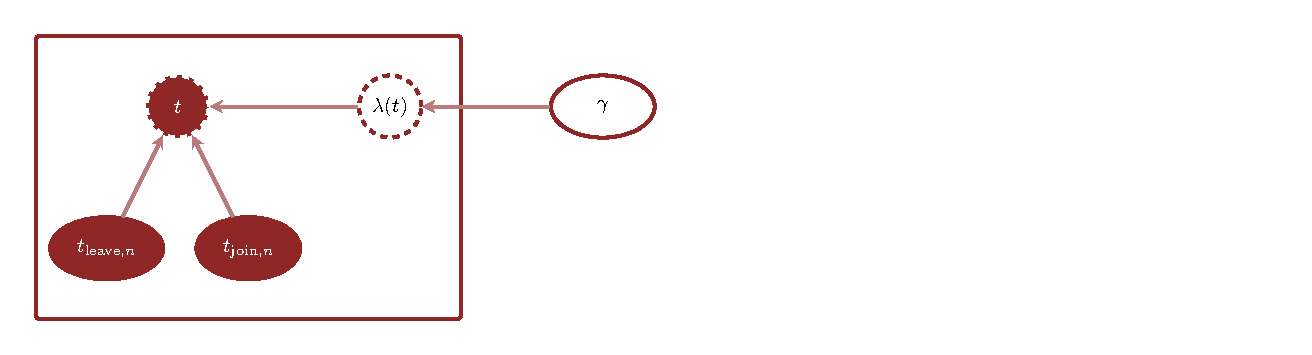
\includegraphics[width=1\textwidth,height=\textheight]{figures/dgms/model1/model1.pdf}

}

\caption{\label{fig-model1}Our initial survival model concerns how long
a customer stays after joining, \(t_{\text{leave}} - t_{\text{join}}\).}

\end{figure}%

\begin{codelisting}

\caption{\texttt{model1.stan}}

\begin{Shaded}
\begin{Highlighting}[]
\KeywordTok{functions}\NormalTok{ \{}
  \CommentTok{// Log stimulus function}
  \DataTypeTok{real}\NormalTok{ log\_lambda(}\DataTypeTok{real}\NormalTok{ t, }\DataTypeTok{real}\NormalTok{ gamma) \{}
    \ControlFlowTok{return}\NormalTok{ log(gamma);}
\NormalTok{  \}}
  
  \CommentTok{// Cumulative stimulus function}
  \DataTypeTok{real}\NormalTok{ Lambda(}\DataTypeTok{real}\NormalTok{ t, }\DataTypeTok{real}\NormalTok{ gamma) \{}
    \ControlFlowTok{return}\NormalTok{ gamma * t;}
\NormalTok{  \}}

  \CommentTok{// Log survival function}
  \DataTypeTok{real}\NormalTok{ log\_survival(}\DataTypeTok{real}\NormalTok{ t, }\DataTypeTok{real}\NormalTok{ gamma) \{}
    \ControlFlowTok{return}\NormalTok{ {-}Lambda(t, gamma);}
\NormalTok{  \}}

  \CommentTok{// Inverse cumulative stimulus function}
  \DataTypeTok{real}\NormalTok{ Lambda\_inv(}\DataTypeTok{real}\NormalTok{ l, }\DataTypeTok{real}\NormalTok{ gamma) \{}
    \ControlFlowTok{return}\NormalTok{ l / gamma;}
\NormalTok{  \}}
  
  \CommentTok{// Inverse survival function}
  \DataTypeTok{real}\NormalTok{ inv\_survival(}\DataTypeTok{real}\NormalTok{ u, }\DataTypeTok{real}\NormalTok{ gamma) \{}
    \ControlFlowTok{return}\NormalTok{ Lambda\_inv({-}log(u), gamma);}
\NormalTok{  \}}
\NormalTok{\}}

\KeywordTok{data}\NormalTok{ \{}
  \DataTypeTok{real}\NormalTok{           T0; }\CommentTok{// Months}
  \DataTypeTok{real}\NormalTok{\textless{}}\KeywordTok{lower}\NormalTok{=T0\textgreater{} T1; }\CommentTok{// Months}

  \CommentTok{// Churned customers}
  \DataTypeTok{int}\NormalTok{\textless{}}\KeywordTok{lower}\NormalTok{=}\DecValTok{0}\NormalTok{\textgreater{} N\_churn;}
  \DataTypeTok{array}\NormalTok{[N\_churn] }\DataTypeTok{real}\NormalTok{\textless{}}\KeywordTok{lower}\NormalTok{=T0, }\KeywordTok{upper}\NormalTok{=T1\textgreater{} t\_join\_churn;  }\CommentTok{// Months}
  \DataTypeTok{array}\NormalTok{[N\_churn] }\DataTypeTok{real}\NormalTok{\textless{}}\KeywordTok{lower}\NormalTok{=T0, }\KeywordTok{upper}\NormalTok{=T1\textgreater{} t\_leave\_churn; }\CommentTok{// Months}
\NormalTok{\}}

\KeywordTok{parameters}\NormalTok{ \{}
  \DataTypeTok{real}\NormalTok{\textless{}}\KeywordTok{lower}\NormalTok{=}\DecValTok{0}\NormalTok{\textgreater{} eta; }\CommentTok{// Inverse scale parameter (Months)}
\NormalTok{\}}

\KeywordTok{transformed parameters}\NormalTok{ \{}
  \DataTypeTok{real}\NormalTok{\textless{}}\KeywordTok{lower}\NormalTok{=}\DecValTok{0}\NormalTok{\textgreater{} gamma = }\DecValTok{1}\NormalTok{ / eta;}
\NormalTok{\}}

\KeywordTok{model}\NormalTok{ \{}
  \CommentTok{// Prior Model}
  \CommentTok{// 0 \textless{}\textasciitilde{} eta \textless{}\textasciitilde{} 40}
  \KeywordTok{target +=}\NormalTok{ normal\_lpdf(eta | }\DecValTok{0}\NormalTok{, }\DecValTok{1}\NormalTok{ / }\FloatTok{2.57}\NormalTok{);}

  \CommentTok{// Observational Model}
  \ControlFlowTok{for}\NormalTok{ (n }\ControlFlowTok{in} \DecValTok{1}\NormalTok{:N\_churn) \{}
    \DataTypeTok{real}\NormalTok{ tenure = t\_leave\_churn[n] {-} t\_join\_churn[n];}
    \KeywordTok{target +=}\NormalTok{   log\_lambda(tenure, gamma)}
\NormalTok{              + log\_survival(tenure, gamma);}
\NormalTok{  \}}
\NormalTok{\}}

\KeywordTok{generated quantities}\NormalTok{ \{}
  \DataTypeTok{array}\NormalTok{[N\_churn] }\DataTypeTok{real}\NormalTok{\textless{}}\KeywordTok{lower}\NormalTok{=}\DecValTok{0}\NormalTok{\textgreater{} tenure\_churn\_pred;}
  \DataTypeTok{array}\NormalTok{[N\_churn] }\DataTypeTok{real}\NormalTok{\textless{}}\KeywordTok{lower}\NormalTok{=T0\textgreater{} t\_leave\_churn\_pred;}

  \ControlFlowTok{for}\NormalTok{ (n }\ControlFlowTok{in} \DecValTok{1}\NormalTok{:N\_churn) \{}
\NormalTok{    tenure\_churn\_pred[n]}
\NormalTok{      = inv\_survival(uniform\_rng(}\DecValTok{0}\NormalTok{, }\DecValTok{1}\NormalTok{), gamma);}
\NormalTok{    t\_leave\_churn\_pred[n]}
\NormalTok{      = t\_join\_churn[n] + tenure\_churn\_pred[n];}
\NormalTok{  \}}
\NormalTok{\}}
\end{Highlighting}
\end{Shaded}

\end{codelisting}

Given the full Bayesian model, we can construct a posterior distribution
that quantifies how consistent each model configuration is with the
observed data.

\begin{Shaded}
\begin{Highlighting}[]
\NormalTok{numeric\_keys }\OperatorTok{=}\NormalTok{ [}\StringTok{\textquotesingle{}T0\textquotesingle{}}\NormalTok{, }\StringTok{\textquotesingle{}T1\textquotesingle{}}\NormalTok{, }\StringTok{\textquotesingle{}I\textquotesingle{}}\NormalTok{, }\StringTok{\textquotesingle{}N\_churn\textquotesingle{}}\NormalTok{, }\StringTok{\textquotesingle{}X\_churn\textquotesingle{}}\NormalTok{,}
                \StringTok{\textquotesingle{}online\_banking\_churn\textquotesingle{}}\NormalTok{, }\StringTok{\textquotesingle{}t\_join\_churn\textquotesingle{}}\NormalTok{,}
                \StringTok{\textquotesingle{}t\_leave\_churn\textquotesingle{}}\NormalTok{, }\StringTok{\textquotesingle{}N\_active\textquotesingle{}}\NormalTok{, }\StringTok{\textquotesingle{}X\_active\textquotesingle{}}\NormalTok{,}
                \StringTok{\textquotesingle{}online\_banking\_active\textquotesingle{}}\NormalTok{, }\StringTok{\textquotesingle{}t\_join\_active\textquotesingle{}}\NormalTok{]}
\NormalTok{stan\_data }\OperatorTok{=}\NormalTok{ \{k: data[k] }\ControlFlowTok{for}\NormalTok{ k }\KeywordTok{in}\NormalTok{ numeric\_keys\}}
\end{Highlighting}
\end{Shaded}

In practice, we'll use \texttt{Stan}'s Hamiltonian Monte Carlo sampler
to quantify the shape of the posterior distribution.

\begin{Shaded}
\begin{Highlighting}[]
\ControlFlowTok{with} \BuiltInTok{open}\NormalTok{(}\StringTok{\textquotesingle{}stan\_programs/model1.stan\textquotesingle{}}\NormalTok{, }\StringTok{\textquotesingle{}r\textquotesingle{}}\NormalTok{) }\ImportTok{as} \BuiltInTok{file}\NormalTok{:}
\NormalTok{  stan\_program }\OperatorTok{=} \BuiltInTok{file}\NormalTok{.read()}
\NormalTok{model }\OperatorTok{=}\NormalTok{ stan.build(stan\_program,}
\NormalTok{                   random\_seed}\OperatorTok{=}\DecValTok{8438338}\NormalTok{,}
\NormalTok{                   data}\OperatorTok{=}\NormalTok{stan\_data)}
\NormalTok{fit }\OperatorTok{=}\NormalTok{ model.sample(num\_samples}\OperatorTok{=}\DecValTok{1024}\NormalTok{, refresh}\OperatorTok{=}\DecValTok{0}\NormalTok{)}
\end{Highlighting}
\end{Shaded}

\begin{verbatim}
Building...
\end{verbatim}

As powerful as Hamiltonian Monte Carlo is, the accuracy of this
posterior quantification is not guaranteed. To ensure faithful posterior
inferences, we have to first review the available computational
diagnostics. In this case, there fortunately don't appear to be any
signs of computational problems.

\begin{Shaded}
\begin{Highlighting}[]
\NormalTok{diagnostics }\OperatorTok{=}\NormalTok{ util.extract\_hmc\_diagnostics(fit)}
\NormalTok{util.check\_all\_hmc\_diagnostics(diagnostics)}

\NormalTok{samples }\OperatorTok{=}\NormalTok{ util.extract\_expectand\_vals(fit)}
\NormalTok{base\_samples }\OperatorTok{=}\NormalTok{ util.filter\_expectands(samples, [}\StringTok{\textquotesingle{}eta\textquotesingle{}}\NormalTok{])}
\NormalTok{util.check\_all\_expectand\_diagnostics(base\_samples)}
\end{Highlighting}
\end{Shaded}

\begin{verbatim}
All Hamiltonian Monte Carlo diagnostics are consistent with accurate
Markov chain Monte Carlo.
 
All expectands checked appear to be behaving well enough for reliable
Markov chain Monte Carlo estimation.
 
\end{verbatim}

\subsection{Posterior Retrodictive
Checks}\label{posterior-retrodictive-checks}

Before reviewing any posterior inferences, we first have to judge the
\href{http://www.symplectomorphic.com/assets/case_studies/principled_bayesian_workflow.html\#143_Posterior_Retrodiction_Checks}{posterior
retrodictive performance} of our model. This requires investigating how
well the posterior predictive distribution recovers various features of
the observed data. Inferences drawn from a model with poor retrodictive
performance poorly describe the actual system being analyzed.

Here the posterior predictive distribution of tenures skews towards
smaller tenures more strongly than what we see in the observed data.

\begin{Shaded}
\begin{Highlighting}[]
\NormalTok{putil.plot\_hist\_quantiles(}
\NormalTok{  plot.gca(), samples, }\StringTok{\textquotesingle{}tenure\_churn\_pred\textquotesingle{}}\NormalTok{,}
\NormalTok{  data[}\StringTok{\textquotesingle{}T0\textquotesingle{}}\NormalTok{] }\OperatorTok{{-}} \DecValTok{1}\NormalTok{, data[}\StringTok{\textquotesingle{}T1\textquotesingle{}}\NormalTok{] }\OperatorTok{+} \DecValTok{1}\NormalTok{, }\DecValTok{1}\NormalTok{,}
\NormalTok{  baseline\_values}\OperatorTok{=}\NormalTok{tenure\_churn,}
\NormalTok{  xlabel}\OperatorTok{=}\StringTok{\textquotesingle{}Customer Tenure (months)\textquotesingle{}}
\NormalTok{)}
\NormalTok{plot.show()}
\end{Highlighting}
\end{Shaded}

\begin{verbatim}
25 predictive values (0.00%) fell above the histogram binning.
\end{verbatim}

\includegraphics{churn_files/figure-pdf/cell-24-output-2.png}

On their own, the posterior predictive leave times not only decay too
quickly, but also extend into impossible values! This suggests that we
might not be properly accounting for the constraints of the finite
observation period.

\begin{Shaded}
\begin{Highlighting}[]
\NormalTok{putil.plot\_hist\_quantiles(}
\NormalTok{  plot.gca(), samples, }\StringTok{\textquotesingle{}t\_leave\_churn\_pred\textquotesingle{}}\NormalTok{,}
\NormalTok{  data[}\StringTok{\textquotesingle{}T0\textquotesingle{}}\NormalTok{] }\OperatorTok{{-}} \DecValTok{3}\NormalTok{, data[}\StringTok{\textquotesingle{}T1\textquotesingle{}}\NormalTok{] }\OperatorTok{+} \DecValTok{23}\NormalTok{, }\DecValTok{3}\NormalTok{,}
\NormalTok{  baseline\_values}\OperatorTok{=}\NormalTok{data[}\StringTok{\textquotesingle{}t\_leave\_churn\textquotesingle{}}\NormalTok{],}
\NormalTok{  xlabel}\OperatorTok{=}\StringTok{"Time Customer Leaves (months)"}
\NormalTok{)}
\NormalTok{plot.gca().axvline(x}\OperatorTok{=}\NormalTok{data[}\StringTok{\textquotesingle{}T0\textquotesingle{}}\NormalTok{], linewidth}\OperatorTok{=}\DecValTok{2}\NormalTok{,}
\NormalTok{                   linestyle}\OperatorTok{=}\StringTok{\textquotesingle{}dashed\textquotesingle{}}\NormalTok{, color}\OperatorTok{=}\StringTok{"\#DDDDDD"}\NormalTok{)}
\NormalTok{plot.gca().axvline(x}\OperatorTok{=}\NormalTok{data[}\StringTok{\textquotesingle{}T1\textquotesingle{}}\NormalTok{], linewidth}\OperatorTok{=}\DecValTok{2}\NormalTok{,}
\NormalTok{                   linestyle}\OperatorTok{=}\StringTok{\textquotesingle{}dashed\textquotesingle{}}\NormalTok{, color}\OperatorTok{=}\StringTok{"\#DDDDDD"}\NormalTok{)}

\NormalTok{plot.show()}
\end{Highlighting}
\end{Shaded}

\begin{verbatim}
2414 predictive values (0.03%) fell above the histogram binning.
\end{verbatim}

\includegraphics{churn_files/figure-pdf/cell-25-output-2.png}

Although we haven't included demographic heterogeneity in our model, we
can still see if the posterior predictions behave similarly to the
observed data across the demographics. Here we'll compare median tenure
in bins of each demographic variable; for a more detailed discussion of
this summary see
\href{http://www.symplectomorphic.com/assets/case_studies/taylor_models.html\#25_Posterior_Retrodictive_Checks}{this
section}.

\begin{Shaded}
\begin{Highlighting}[]
\NormalTok{bin\_min }\OperatorTok{=}\NormalTok{ [ }\DecValTok{0}\NormalTok{, }\DecValTok{0}\NormalTok{, }\DecValTok{0}\NormalTok{, }\DecValTok{0}\NormalTok{ ]}
\NormalTok{bin\_max }\OperatorTok{=}\NormalTok{ [ }\DecValTok{100}\NormalTok{, }\DecValTok{15}\NormalTok{, }\FloatTok{1.05}\NormalTok{, }\DecValTok{1000}\NormalTok{ ]}
\NormalTok{bin\_delta }\OperatorTok{=}\NormalTok{ [ }\DecValTok{20}\NormalTok{, }\DecValTok{1}\NormalTok{, }\FloatTok{0.20}\NormalTok{, }\DecValTok{200}\NormalTok{ ]}

\NormalTok{pred\_names }\OperatorTok{=}\NormalTok{ [ }\SpecialStringTok{f\textquotesingle{}tenure\_churn\_pred[}\SpecialCharTok{\{}\NormalTok{n }\OperatorTok{+} \DecValTok{1}\SpecialCharTok{\}}\SpecialStringTok{]\textquotesingle{}}
               \ControlFlowTok{for}\NormalTok{ n }\KeywordTok{in} \BuiltInTok{range}\NormalTok{(data[}\StringTok{\textquotesingle{}N\_churn\textquotesingle{}}\NormalTok{]) ]}

\NormalTok{f, axarr }\OperatorTok{=}\NormalTok{ plot.subplots(}\DecValTok{2}\NormalTok{, }\DecValTok{2}\NormalTok{, layout}\OperatorTok{=}\StringTok{"constrained"}\NormalTok{)}

\ControlFlowTok{for}\NormalTok{ i }\KeywordTok{in} \BuiltInTok{range}\NormalTok{(data[}\StringTok{\textquotesingle{}I\textquotesingle{}}\NormalTok{]):}
\NormalTok{  i1 }\OperatorTok{=}\NormalTok{ i }\OperatorTok{//} \DecValTok{2}
\NormalTok{  i2 }\OperatorTok{=}\NormalTok{ i }\OperatorTok{\%} \DecValTok{2}

\NormalTok{  putil.plot\_conditional\_median\_quantiles(}
\NormalTok{    axarr[i1, i2], samples, pred\_names,}
\NormalTok{    [ x[i] }\ControlFlowTok{for}\NormalTok{ x }\KeywordTok{in}\NormalTok{ data[}\StringTok{\textquotesingle{}X\_churn\textquotesingle{}}\NormalTok{] ],}
\NormalTok{    bin\_min[i], bin\_max[i], bin\_delta[i],}
\NormalTok{    tenure\_churn, residual}\OperatorTok{=}\VariableTok{False}\NormalTok{,}
\NormalTok{    xlabel}\OperatorTok{=}\NormalTok{data[}\StringTok{\textquotesingle{}x\_names\textquotesingle{}}\NormalTok{][i], ylabel}\OperatorTok{=}\StringTok{""}
\NormalTok{  )}

\NormalTok{plot.show()}
\end{Highlighting}
\end{Shaded}

\begin{verbatim}
1 conditioning values (0.04%) fell below the histogram binning.
6 conditioning values (0.27%) fell above the histogram binning.
\end{verbatim}

\includegraphics{churn_files/figure-pdf/cell-26-output-2.png}

There is clear retrodictive disagreement here, as well.

\section{Model 2: Constant Stimulus/Hazard Model with
Censoring}\label{model-2-constant-stimulushazard-model-with-censoring}

All of this poor retrodictive performance indicates that our initial
model is nowhere near adequate enough to fit the observed data.
Fortunately, the precise nature of the retrodictive tensions motivates a
variety of explicit improvements to our model.

Let's start by addressing the impossible posterior predictions for the
customer leave times. Predicted leave times for churned customers have
to be \emph{before} the end of the observational window, otherwise those
customers would still be active.

At the same time, we are not completely ignorant of the leave times of
the active customers. They must be after the close of the observational
period.

Conveniently, both of these behaviors are straightforward to accommodate
into our survival model.

\subsection{Censored Observational
Model}\label{censored-observational-model}

When making predictions for churned customers, \(t_{\text{leave}}\) has
to be smaller than the right observational boundary \(T_{1}\), \[
t_{\text{leave}} < T_{1}.
\] This then constrains the possible tenures; if the customer joined at
\(t_{\text{join}}\) then \begin{align*}
t_{\text{leave}} &< T_{1}
\\
t_{\text{leave}} - t_{\text{join}} &< T_{1} - t_{\text{join}}
\\
t &< T_{1} - t_{\text{join}}.
\end{align*} In other words, we have to \emph{truncate} the
time-to-event model when making predictions.

To accommodate active customers, we can treat their unobserved leave
times as auxiliary parameters that we then marginalize. For a single
active customer, the leave time model is given by \[
p( t_{\text{leave}} \mid t_{\text{join}}, \theta )
=
p( t_{\text{leave}} - t_{\text{join}} \mid \theta ),
\] where \(p( t \mid \theta )\) is the time-to-event model. To
marginalize the unobserved \(t_{\text{leave}}\), we integrate over the
possible values, \begin{align*}
\int_{T_{1}}^{\infty} \mathrm{d} t_{\text{leave}} \,
p( t_{\text{leave}} \mid t_{\text{join}}, \theta )
\\
&=
\int_{T_{1}}^{\infty} \mathrm{d} t_{\text{leave}} \,
p( t_{\text{leave}} - t_{\text{join}} \mid \theta )
\\
&=
\int_{T_{1} - t_{\text{join}}}^{\infty} \mathrm{d} t \,
p( t \mid \theta )
\\
&=
\pi[ t > T_{1} - t_{\text{join}} ]
\\
&=
S( T_{1} - t_{\text{join}} ).
\end{align*}

In other words, each active customer doesn't contribute a point-wise
density \(p(t)\) to the observational model, but rather an entire
interval probability \(\pi[ t > T_{1} - t_{\text{join}} ]\).

\subsection{Posterior Quantification}\label{posterior-quantification-1}

With a bit more care, our full Bayesian model now considers both the
churned and active customers (Figure~\ref{fig-model2}).

\begin{figure}

\centering{

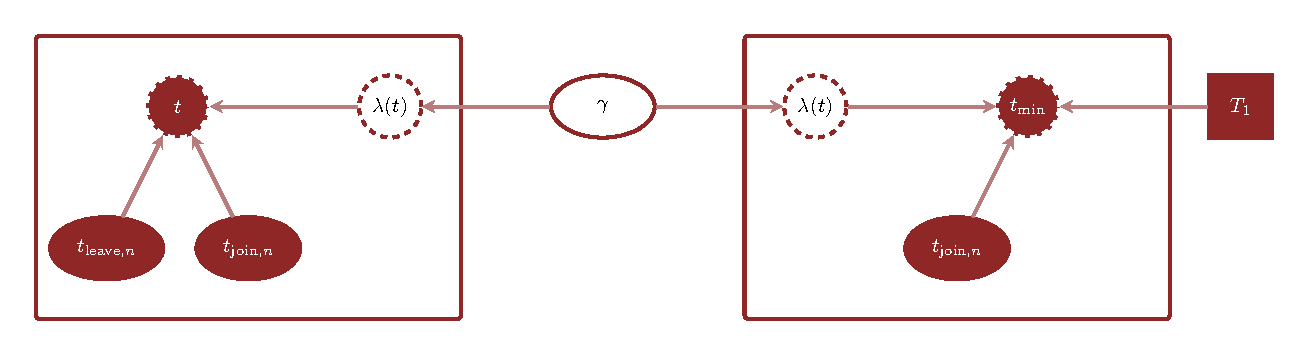
\includegraphics[width=1\textwidth,height=\textheight]{figures/dgms/model2/model2.pdf}

}

\caption{\label{fig-model2}Although we don't observe the precise leave
times of the active customers, we can lower bound them by how far the
join times are from the end of the observation period. These censored
observations also inform the parameters of our survival model.}

\end{figure}%

Conveniently, censored observations and predictions can both be
implemented with the log survival function.

\begin{codelisting}

\caption{\texttt{model2.stan}}

\begin{Shaded}
\begin{Highlighting}[]
\KeywordTok{functions}\NormalTok{ \{}
  \CommentTok{// Log stimulus function}
  \DataTypeTok{real}\NormalTok{ log\_lambda(}\DataTypeTok{real}\NormalTok{ t, }\DataTypeTok{real}\NormalTok{ gamma) \{}
    \ControlFlowTok{return}\NormalTok{ log(gamma);}
\NormalTok{  \}}
  
  \CommentTok{// Cumulative stimulus function}
  \DataTypeTok{real}\NormalTok{ Lambda(}\DataTypeTok{real}\NormalTok{ t, }\DataTypeTok{real}\NormalTok{ gamma) \{}
    \ControlFlowTok{return}\NormalTok{ gamma * t;}
\NormalTok{  \}}

  \CommentTok{// Log survival function}
  \DataTypeTok{real}\NormalTok{ log\_survival(}\DataTypeTok{real}\NormalTok{ t, }\DataTypeTok{real}\NormalTok{ gamma) \{}
    \ControlFlowTok{return}\NormalTok{ {-}Lambda(t, gamma);}
\NormalTok{  \}}

  \CommentTok{// Inverse cumulative stimulus function}
  \DataTypeTok{real}\NormalTok{ Lambda\_inv(}\DataTypeTok{real}\NormalTok{ l, }\DataTypeTok{real}\NormalTok{ gamma) \{}
    \ControlFlowTok{return}\NormalTok{ l / gamma;}
\NormalTok{  \}}
  
  \CommentTok{// Inverse survival function}
  \DataTypeTok{real}\NormalTok{ inv\_survival(}\DataTypeTok{real}\NormalTok{ u, }\DataTypeTok{real}\NormalTok{ gamma) \{}
    \ControlFlowTok{return}\NormalTok{ Lambda\_inv({-}log(u), gamma);}
\NormalTok{  \}}
\NormalTok{\}}

\KeywordTok{data}\NormalTok{ \{}
  \DataTypeTok{real}\NormalTok{           T0; }\CommentTok{// Months}
  \DataTypeTok{real}\NormalTok{\textless{}}\KeywordTok{lower}\NormalTok{=T0\textgreater{} T1; }\CommentTok{// Months}

  \CommentTok{// Churned customers}
  \DataTypeTok{int}\NormalTok{\textless{}}\KeywordTok{lower}\NormalTok{=}\DecValTok{0}\NormalTok{\textgreater{} N\_churn;}
  \DataTypeTok{array}\NormalTok{[N\_churn] }\DataTypeTok{real}\NormalTok{\textless{}}\KeywordTok{lower}\NormalTok{=T0, }\KeywordTok{upper}\NormalTok{=T1\textgreater{} t\_join\_churn;  }\CommentTok{// Months}
  \DataTypeTok{array}\NormalTok{[N\_churn] }\DataTypeTok{real}\NormalTok{\textless{}}\KeywordTok{lower}\NormalTok{=T0, }\KeywordTok{upper}\NormalTok{=T1\textgreater{} t\_leave\_churn; }\CommentTok{// Months}

  \CommentTok{// Active customers}
  \DataTypeTok{int}\NormalTok{\textless{}}\KeywordTok{lower}\NormalTok{=}\DecValTok{0}\NormalTok{\textgreater{} N\_active;}
  \DataTypeTok{array}\NormalTok{[N\_active] }\DataTypeTok{real}\NormalTok{\textless{}}\KeywordTok{lower}\NormalTok{=T0, }\KeywordTok{upper}\NormalTok{=T1\textgreater{} t\_join\_active; }\CommentTok{// Months}
\NormalTok{\}}

\KeywordTok{parameters}\NormalTok{ \{}
  \DataTypeTok{real}\NormalTok{\textless{}}\KeywordTok{lower}\NormalTok{=}\DecValTok{0}\NormalTok{\textgreater{} eta; }\CommentTok{// Inverse scale parameter (Months)}
\NormalTok{\}}

\KeywordTok{transformed parameters}\NormalTok{ \{}
  \DataTypeTok{real}\NormalTok{\textless{}}\KeywordTok{lower}\NormalTok{=}\DecValTok{0}\NormalTok{\textgreater{} gamma = }\DecValTok{1}\NormalTok{ / eta;}
\NormalTok{\}}

\KeywordTok{model}\NormalTok{ \{}
  \CommentTok{// Prior Model}
  \CommentTok{// 0 \textless{}\textasciitilde{} eta \textless{}\textasciitilde{} 40}
  \KeywordTok{target +=}\NormalTok{ normal\_lpdf(eta | }\DecValTok{0}\NormalTok{, }\DecValTok{1}\NormalTok{ / }\FloatTok{2.57}\NormalTok{);}

  \CommentTok{// Observational Model}
  \ControlFlowTok{for}\NormalTok{ (n }\ControlFlowTok{in} \DecValTok{1}\NormalTok{:N\_churn) \{}
    \DataTypeTok{real}\NormalTok{ tenure = t\_leave\_churn[n] {-} t\_join\_churn[n];}
    \KeywordTok{target +=}\NormalTok{   log\_lambda(tenure, gamma)}
\NormalTok{              + log\_survival(tenure, gamma);}
\NormalTok{  \}}

  \ControlFlowTok{for}\NormalTok{ (n }\ControlFlowTok{in} \DecValTok{1}\NormalTok{:N\_active) \{}
    \KeywordTok{target +=}\NormalTok{ log\_survival(T1 {-} t\_join\_active[n], gamma);}
\NormalTok{  \}}
\NormalTok{\}}

\KeywordTok{generated quantities}\NormalTok{ \{}
  \DataTypeTok{array}\NormalTok{[N\_churn] }\DataTypeTok{real}\NormalTok{\textless{}}\KeywordTok{lower}\NormalTok{=}\DecValTok{0}\NormalTok{\textgreater{} tenure\_churn\_pred;}
  \DataTypeTok{array}\NormalTok{[N\_churn] }\DataTypeTok{real}\NormalTok{\textless{}}\KeywordTok{lower}\NormalTok{=T0\textgreater{} t\_leave\_churn\_pred;}

  \ControlFlowTok{for}\NormalTok{ (n }\ControlFlowTok{in} \DecValTok{1}\NormalTok{:N\_churn) \{}
    \DataTypeTok{real}\NormalTok{ S = exp(log\_survival(T1 {-} t\_join\_churn[n], gamma));}
    \DataTypeTok{real}\NormalTok{ u = uniform\_rng(S, }\DecValTok{1}\NormalTok{);}
\NormalTok{    tenure\_churn\_pred[n]}
\NormalTok{      = inv\_survival(u, gamma);}
\NormalTok{    t\_leave\_churn\_pred[n]}
\NormalTok{      = t\_join\_churn[n] + tenure\_churn\_pred[n];}
\NormalTok{  \}}
\NormalTok{\}}
\end{Highlighting}
\end{Shaded}

\end{codelisting}

\begin{Shaded}
\begin{Highlighting}[]
\ControlFlowTok{with} \BuiltInTok{open}\NormalTok{(}\StringTok{\textquotesingle{}stan\_programs/model2.stan\textquotesingle{}}\NormalTok{, }\StringTok{\textquotesingle{}r\textquotesingle{}}\NormalTok{) }\ImportTok{as} \BuiltInTok{file}\NormalTok{:}
\NormalTok{  stan\_program }\OperatorTok{=} \BuiltInTok{file}\NormalTok{.read()}
\NormalTok{model }\OperatorTok{=}\NormalTok{ stan.build(stan\_program,}
\NormalTok{                   random\_seed}\OperatorTok{=}\DecValTok{8438338}\NormalTok{,}
\NormalTok{                   data}\OperatorTok{=}\NormalTok{stan\_data)}
\NormalTok{fit }\OperatorTok{=}\NormalTok{ model.sample(num\_samples}\OperatorTok{=}\DecValTok{1024}\NormalTok{, refresh}\OperatorTok{=}\DecValTok{0}\NormalTok{)}
\end{Highlighting}
\end{Shaded}

\begin{verbatim}
Building...
\end{verbatim}

Despite the added model complexity, no computational problems have
arisen when we quantify the resulting posterior distribution.
Hamiltonian Monte Carlo is well-suited for exploring complex posterior
distributions!

\begin{Shaded}
\begin{Highlighting}[]
\NormalTok{diagnostics }\OperatorTok{=}\NormalTok{ util.extract\_hmc\_diagnostics(fit)}
\NormalTok{util.check\_all\_hmc\_diagnostics(diagnostics)}

\NormalTok{samples }\OperatorTok{=}\NormalTok{ util.extract\_expectand\_vals(fit)}
\NormalTok{base\_samples }\OperatorTok{=}\NormalTok{ util.filter\_expectands(samples, [}\StringTok{\textquotesingle{}eta\textquotesingle{}}\NormalTok{])}
\NormalTok{util.check\_all\_expectand\_diagnostics(base\_samples)}
\end{Highlighting}
\end{Shaded}

\begin{verbatim}
All Hamiltonian Monte Carlo diagnostics are consistent with accurate
Markov chain Monte Carlo.
 
All expectands checked appear to be behaving well enough for reliable
Markov chain Monte Carlo estimation.
 
\end{verbatim}

\subsection{Posterior Retrodictive
Checks}\label{posterior-retrodictive-checks-1}

Did these changes improve the adequacy of our model at all? Well, the
posterior predictive leave times now agree much better with the observed
behavior.

\begin{Shaded}
\begin{Highlighting}[]
\NormalTok{putil.plot\_hist\_quantiles(}
\NormalTok{  plot.gca(), samples, }\StringTok{\textquotesingle{}t\_leave\_churn\_pred\textquotesingle{}}\NormalTok{,}
\NormalTok{  data[}\StringTok{\textquotesingle{}T0\textquotesingle{}}\NormalTok{] }\OperatorTok{{-}} \DecValTok{3}\NormalTok{, data[}\StringTok{\textquotesingle{}T1\textquotesingle{}}\NormalTok{] }\OperatorTok{+} \DecValTok{23}\NormalTok{, }\DecValTok{3}\NormalTok{,}
\NormalTok{  baseline\_values}\OperatorTok{=}\NormalTok{data[}\StringTok{\textquotesingle{}t\_leave\_churn\textquotesingle{}}\NormalTok{],}
\NormalTok{  xlabel}\OperatorTok{=}\StringTok{"Time Customer Leaves (months)"}
\NormalTok{)}
\NormalTok{plot.gca().axvline(x}\OperatorTok{=}\NormalTok{data[}\StringTok{\textquotesingle{}T0\textquotesingle{}}\NormalTok{], linewidth}\OperatorTok{=}\DecValTok{2}\NormalTok{,}
\NormalTok{                   linestyle}\OperatorTok{=}\StringTok{\textquotesingle{}dashed\textquotesingle{}}\NormalTok{, color}\OperatorTok{=}\StringTok{"\#DDDDDD"}\NormalTok{)}
\NormalTok{plot.gca().axvline(x}\OperatorTok{=}\NormalTok{data[}\StringTok{\textquotesingle{}T1\textquotesingle{}}\NormalTok{], linewidth}\OperatorTok{=}\DecValTok{2}\NormalTok{,}
\NormalTok{                   linestyle}\OperatorTok{=}\StringTok{\textquotesingle{}dashed\textquotesingle{}}\NormalTok{, color}\OperatorTok{=}\StringTok{"\#DDDDDD"}\NormalTok{)}

\NormalTok{plot.show()}
\end{Highlighting}
\end{Shaded}

\includegraphics{churn_files/figure-pdf/cell-29-output-1.png}

Unfortunately, there is still tension in the customer tenure.
Specifically, the observed behavior is peaked away from zero while the
posterior predictive behavior peaks at zero.

\begin{Shaded}
\begin{Highlighting}[]
\NormalTok{putil.plot\_hist\_quantiles(}
\NormalTok{  plot.gca(), samples, }\StringTok{\textquotesingle{}tenure\_churn\_pred\textquotesingle{}}\NormalTok{,}
\NormalTok{  data[}\StringTok{\textquotesingle{}T0\textquotesingle{}}\NormalTok{] }\OperatorTok{{-}} \DecValTok{1}\NormalTok{, data[}\StringTok{\textquotesingle{}T1\textquotesingle{}}\NormalTok{] }\OperatorTok{+} \DecValTok{1}\NormalTok{, }\DecValTok{1}\NormalTok{,}
\NormalTok{  baseline\_values}\OperatorTok{=}\NormalTok{tenure\_churn,}
\NormalTok{  xlabel}\OperatorTok{=}\StringTok{\textquotesingle{}Customer Tenure (months)\textquotesingle{}}
\NormalTok{)}
\NormalTok{plot.show()}
\end{Highlighting}
\end{Shaded}

\includegraphics{churn_files/figure-pdf/cell-30-output-1.png}

Reflecting on our model, the exponential time-to-event model
\emph{always} peaks at zero. In other words, there is no configuration
of our current survival model that can match this observed behavior.

Let's try to address this inadequacy before we consider the retrodictive
performance across the demographic variables.

\section{Model 3: Power Stimulus/Hazard Model with
Censoring}\label{model-3-power-stimulushazard-model-with-censoring}

Fortunately, our initial survival model isn't too difficult to
generalize.

\subsection{Observational Model}\label{observational-model-1}

Instead of a constant stimulus, let's allow the stimulus to potentially
increase with a power of time, \[
\lambda(t)
=
\alpha \, \frac{1}{\sigma} \,
\left( \frac{t}{\sigma} \right)^{\alpha - 1}
\] This results in the cumulative stimulus function \[
\Lambda(t)
=
\int_{0}^{t} \mathrm{d} t' \, \lambda(t')
=
\left( \frac{t}{\sigma} \right)^{\alpha},
\] and the survival function \[
S(t)
=
\exp \left( - \Lambda(t) \right)
=
\exp \left( - \left( \frac{t}{\sigma} \right)^{\alpha} \right).
\]

Interestingly, the generalized time-to-event model also reduces to a
familiar form, this time the Weibull family of probability density
functions, \begin{align*}
p(t)
&=
\lambda(t) \, S(t)
\\
&=
\alpha \, \frac{1}{\sigma} \,
\left( \frac{t}{\sigma} \right)^{\alpha - 1} \,
\exp \left( - \left( \frac{t}{\sigma} \right)^{\alpha} \right)
\\
&= \mathrm{Weibull}(t \mid \alpha, \sigma).
\end{align*}

Note that if \(\alpha = 1\) then this model reduces to our initial
exponential model with \(\lambda = 1 / \sigma\). Because we've
\emph{expanded} our model, we're allowing our inferences to consider
more complex behaviors, but not forcing it to.

\subsection{Prior Model}\label{prior-model-1}

The single threshold that we considered before was enough to constrain
the reasonable configurations of \(\gamma\) in our initial model. It is
not, however, sufficient to constrain both \(\alpha\) and \(\sigma\) in
our generalized model.

Here we'll elicit addition domain expertise to inform \emph{two}
thresholds: one suppressing unreasonably large tenures, and one
suppressing unreasonably small tenures. Let's say that customers leaving
before only a single month should be rare.

This gives us two tail probability constraints, \begin{align*}
\pi( t < 1 \text{ month } ) \approx 0.01
\\
\pi( t > 60 \text{ months } ) \approx 0.01,
\end{align*} which gives us two equations for the reasonable values of
\(\alpha\) and \(\sigma\).

First we have \begin{align*}
S( 1 \text{ month }) &= 0.99
\\
\exp \left(
  -\left( \frac{ 1 \text{ month } }{ \sigma } \right)^\alpha
\right)
&=
0.99
\\
\left( \frac{ 1 \text{ month } }{ \sigma } \right)^\alpha
&=
-\log(0.99)
\\
-\alpha \, \log \left( \frac{ \sigma }{ 1 \text{ month } } \right)
&=
\log(-\log(0.99))
\\
\alpha \, \log \left( \frac{ \sigma }{ 1 \text{ month } } \right)
&=
-\log(-\log(0.99)).
\end{align*} Second we have \begin{align*}
S( 60 \text{ months }) &= 0.01
\\
\exp \left(
  -\left( \frac{ 60 \text{ months } }{ \sigma } \right)^\alpha
\right)
&=
0.01
\\
\left( \frac{ 60 \text{ months } }{ \sigma } \right)^\alpha
&=
-\log(0.01)
\\
-\alpha \, \log \left( \frac{ \sigma }{ 60 \text{ months } } \right)
&=
\log(-\log(0.01))
\\
\alpha \, \log \left( \frac{ \sigma }{ 60 \text{ months } } \right)
&=
-\log(-\log(0.01)).
\end{align*}

After first defining \[
\kappa = \frac{ \log(-\log(0.99)) }{ \log(-\log(0.01)) },
\] we can divide the two equations to give an equation entirely in terms
of \(\sigma\), \begin{align*}
\frac{
  \log \left( \frac{ \sigma }{ 1 \text{ month } } \right)
}{
  \log \left( \frac{ \sigma }{ 1 \text{ month } } \right)
  - \log 60
}
&=
\kappa
\\
\log \left( \frac{ \sigma }{ 1 \text{ month } } \right)
&=
  \kappa \, \log \left( \frac{ \sigma }{ 1 \text{ month } } \right)
- \kappa \, \log 60
\\
( 1 - \kappa ) \,
\log \left( \frac{ \sigma }{ 1 \text{ month } } \right)
&=
- \kappa \, \log 60
\\
\log \left( \frac{ \sigma }{ 1 \text{ month } } \right)
&=
- \frac{ \kappa }{ 1 - \kappa} \, \log 60
\\
\sigma
&=
60^{- \frac{ \kappa }{ 1 - \kappa} } \text{ month }.
\end{align*}

Model configurations with \(\sigma\) larger than this value will be too
diffuse, allocating excessive probability below and above our two
thresholds.

Next, we can solve the first equation for \(\sigma\), \[
\log( \sigma) = - \frac{ \log(-\log(0.99)) }{ \alpha },
\] and then substitute it into the second equation to give an equation
entirely in terms of \(\alpha\), \begin{align*}
\alpha \,
\log \left( \frac{ \sigma }{ 60 \text{ months } } \right)
&=
-\log(-\log(0.01))
\\
\alpha \,
\log \left( \frac{ \sigma }{ 1 \text{ month } } \right)
- \alpha \, \log 60
&=
-\log(-\log(0.01))
\\
\alpha \,
\left( - \frac{ \log(-\log(0.99)) }{ \alpha } \right)
- \alpha \, \log 60
&=
-\log(-\log(0.01))
\\
- \log(-\log(0.99))
- \alpha \, \log 60
&=
-\log(-\log(0.01))
\\
- \alpha \, \log 60
&=
-\log(-\log(0.01)) + \log(-\log(0.99))
\\
\alpha
&=
\frac{ \log(-\log(0.01)) - \log(-\log(0.99)) }{ \log 60 }.
\end{align*} Model configurations with \(\alpha\) \emph{below} this
value will concentrate at tenures that are too long.

Adding a little bit of a buffer, these calculations suggest the
parameter constraints \[
0 \lessapprox \sigma \lessapprox 75,
\] and \[
1 \lessapprox \alpha.
\] The latter is equivalent to \[
0 \lessapprox \omega = \frac{1}{\alpha} \lessapprox 1.
\]

Once again, half-normal prior models neatly ensure the desired
regularization, \begin{align*}
p( \sigma ) = \text{half-normal}( \sigma \mid 0, 75 / 2.57 )
\\
p( \omega ) = \text{half-normal}( \omega \mid 0, 1 / 2.57)
\end{align*}

We can verify that this prior model behaves as expected by implementing
another prior predictive check.

\begin{Shaded}
\begin{Highlighting}[]
\NormalTok{t\_lower }\OperatorTok{=} \DecValTok{1}
\NormalTok{t\_upper }\OperatorTok{=} \DecValTok{60}
\end{Highlighting}
\end{Shaded}

\begin{codelisting}

\caption{\texttt{model3\textbackslash\_prior.stan}}

\begin{Shaded}
\begin{Highlighting}[]
\KeywordTok{functions}\NormalTok{ \{}
  \CommentTok{// Log stimulus function}
  \DataTypeTok{real}\NormalTok{ log\_lambda(}\DataTypeTok{real}\NormalTok{ t, }\DataTypeTok{real}\NormalTok{ alpha, }\DataTypeTok{real}\NormalTok{ sigma) \{}
    \ControlFlowTok{return}\NormalTok{ log(alpha) {-} log(sigma) + (alpha {-} }\DecValTok{1}\NormalTok{) * log(t / sigma);}
\NormalTok{  \}}
  
  \CommentTok{// Cumulative stimulus function}
  \DataTypeTok{real}\NormalTok{ Lambda(}\DataTypeTok{real}\NormalTok{ t, }\DataTypeTok{real}\NormalTok{ alpha, }\DataTypeTok{real}\NormalTok{ sigma) \{}
    \ControlFlowTok{return}\NormalTok{ pow(t / sigma, alpha);}
\NormalTok{  \}}

  \CommentTok{// Log survival function}
  \DataTypeTok{real}\NormalTok{ log\_survival(}\DataTypeTok{real}\NormalTok{ t, }\DataTypeTok{real}\NormalTok{ alpha, }\DataTypeTok{real}\NormalTok{ sigma) \{}
    \ControlFlowTok{return}\NormalTok{ {-}Lambda(t, alpha, sigma);}
\NormalTok{  \}}

  \CommentTok{// Inverse cumulative stimulus function}
  \DataTypeTok{real}\NormalTok{ Lambda\_inv(}\DataTypeTok{real}\NormalTok{ l, }\DataTypeTok{real}\NormalTok{ alpha, }\DataTypeTok{real}\NormalTok{ sigma) \{}
    \ControlFlowTok{return}\NormalTok{ sigma * pow(l, }\DecValTok{1}\NormalTok{ / alpha);}
\NormalTok{  \}}
  
  \CommentTok{// Inverse survival function}
  \DataTypeTok{real}\NormalTok{ inv\_survival(}\DataTypeTok{real}\NormalTok{ u, }\DataTypeTok{real}\NormalTok{ alpha, }\DataTypeTok{real}\NormalTok{ sigma) \{}
    \ControlFlowTok{return}\NormalTok{ Lambda\_inv({-}log(u), alpha, sigma);}
\NormalTok{  \}}
\NormalTok{\}}

\KeywordTok{data}\NormalTok{ \{}
  \DataTypeTok{int}\NormalTok{\textless{}}\KeywordTok{lower}\NormalTok{=}\DecValTok{0}\NormalTok{\textgreater{} N;}
  \DataTypeTok{real}\NormalTok{\textless{}}\KeywordTok{lower}\NormalTok{=}\DecValTok{0}\NormalTok{\textgreater{} t\_lower;}
  \DataTypeTok{real}\NormalTok{\textless{}}\KeywordTok{lower}\NormalTok{=}\DecValTok{0}\NormalTok{\textgreater{} t\_upper;}
\NormalTok{\}}

\KeywordTok{parameters}\NormalTok{ \{}
  \DataTypeTok{real}\NormalTok{\textless{}}\KeywordTok{lower}\NormalTok{=}\DecValTok{0}\NormalTok{\textgreater{} omega; }\CommentTok{// Inverse shape parameter (Unitless)}
  \DataTypeTok{real}\NormalTok{\textless{}}\KeywordTok{lower}\NormalTok{=}\DecValTok{0}\NormalTok{\textgreater{} sigma; }\CommentTok{// Scale parameter (Months)}
\NormalTok{\}}

\KeywordTok{model}\NormalTok{ \{}
  \CommentTok{// Prior Model}
  \CommentTok{// 1 \textless{}\textasciitilde{} alpha}
  \CommentTok{// 0 \textless{}\textasciitilde{} omega = 1 / alpha \textless{}\textasciitilde{} 1 / 1}
  \KeywordTok{target +=}\NormalTok{ normal\_lpdf(omega | }\DecValTok{0}\NormalTok{, }\DecValTok{1}\NormalTok{ / }\FloatTok{2.57}\NormalTok{);}

  \CommentTok{// 0 \textless{}\textasciitilde{} sigma \textless{}\textasciitilde{} 75}
  \KeywordTok{target +=}\NormalTok{ normal\_lpdf(sigma | }\DecValTok{0}\NormalTok{, }\DecValTok{75}\NormalTok{ / }\FloatTok{2.57}\NormalTok{);}
\NormalTok{\}}

\KeywordTok{generated quantities}\NormalTok{ \{}
  \DataTypeTok{array}\NormalTok{[N] }\DataTypeTok{real}\NormalTok{\textless{}}\KeywordTok{lower}\NormalTok{=}\DecValTok{0}\NormalTok{\textgreater{} tenure\_pred;}
  \DataTypeTok{real}\NormalTok{ lower\_tail\_p\_hat = }\DecValTok{0}\NormalTok{;}
  \DataTypeTok{real}\NormalTok{ upper\_tail\_p\_hat = }\DecValTok{0}\NormalTok{;}

  \ControlFlowTok{for}\NormalTok{ (n }\ControlFlowTok{in} \DecValTok{1}\NormalTok{:N) \{}
\NormalTok{    tenure\_pred[n]}
\NormalTok{      = inv\_survival(uniform\_rng(}\DecValTok{0}\NormalTok{, }\DecValTok{1}\NormalTok{), }\DecValTok{1}\NormalTok{ / omega, sigma);}
    \ControlFlowTok{if}\NormalTok{ (tenure\_pred[n] \textless{} t\_lower)}
\NormalTok{      lower\_tail\_p\_hat += }\DecValTok{1}\NormalTok{;}
    \ControlFlowTok{if}\NormalTok{ (tenure\_pred[n] \textgreater{} t\_upper)}
\NormalTok{      upper\_tail\_p\_hat += }\DecValTok{1}\NormalTok{;}
\NormalTok{  \}}
\NormalTok{  lower\_tail\_p\_hat /= N;}
\NormalTok{  upper\_tail\_p\_hat /= N;}
\NormalTok{\}}
\end{Highlighting}
\end{Shaded}

\end{codelisting}

\begin{Shaded}
\begin{Highlighting}[]
\ControlFlowTok{with} \BuiltInTok{open}\NormalTok{(}\StringTok{\textquotesingle{}stan\_programs/model3\_prior.stan\textquotesingle{}}\NormalTok{, }\StringTok{\textquotesingle{}r\textquotesingle{}}\NormalTok{) }\ImportTok{as} \BuiltInTok{file}\NormalTok{:}
\NormalTok{  stan\_program }\OperatorTok{=} \BuiltInTok{file}\NormalTok{.read()}
\NormalTok{model }\OperatorTok{=}\NormalTok{ stan.build(stan\_program,}
\NormalTok{                   random\_seed}\OperatorTok{=}\DecValTok{8438338}\NormalTok{,}
\NormalTok{                   data}\OperatorTok{=}\NormalTok{\{}\StringTok{\textquotesingle{}N\textquotesingle{}}\NormalTok{: }\DecValTok{2500}\NormalTok{,}
                         \StringTok{\textquotesingle{}t\_lower\textquotesingle{}}\NormalTok{: t\_lower,}
                         \StringTok{\textquotesingle{}t\_upper\textquotesingle{}}\NormalTok{: t\_upper\})}
\NormalTok{fit }\OperatorTok{=}\NormalTok{ model.sample(num\_samples}\OperatorTok{=}\DecValTok{1024}\NormalTok{, refresh}\OperatorTok{=}\DecValTok{0}\NormalTok{)}

\NormalTok{samples }\OperatorTok{=}\NormalTok{ util.extract\_expectand\_vals(fit)}
\end{Highlighting}
\end{Shaded}

\begin{verbatim}
Building...
\end{verbatim}

Qualitatively, the prior predictive behavior is similar to that in our
previous model.

\begin{Shaded}
\begin{Highlighting}[]
\NormalTok{putil.plot\_hist\_quantiles(}
\NormalTok{  plot.gca(), samples, }\StringTok{\textquotesingle{}tenure\_pred\textquotesingle{}}\NormalTok{,}
  \DecValTok{0}\NormalTok{, t\_upper }\OperatorTok{+} \DecValTok{12}\NormalTok{, }\DecValTok{2}\NormalTok{,}
\NormalTok{  xlabel}\OperatorTok{=}\StringTok{\textquotesingle{}Customer Tenure (months)\textquotesingle{}}
\NormalTok{)}
\NormalTok{plot.gca().set\_xlim([}\DecValTok{0}\NormalTok{, t\_upper }\OperatorTok{+} \DecValTok{10}\NormalTok{])}

\NormalTok{rect\_lower }\OperatorTok{=}\NormalTok{ plot.Rectangle((}\DecValTok{0}\NormalTok{, }\DecValTok{0}\NormalTok{), t\_lower, }\DecValTok{1600}\NormalTok{,}
\NormalTok{                      facecolor}\OperatorTok{=}\StringTok{"\#BBBBBB"}\NormalTok{, alpha}\OperatorTok{=}\FloatTok{0.25}\NormalTok{)}
\NormalTok{plot.gca().add\_patch(rect\_lower)}
\NormalTok{plot.axvline(x}\OperatorTok{=}\NormalTok{t\_lower, linewidth}\OperatorTok{=}\DecValTok{2}\NormalTok{, color}\OperatorTok{=}\StringTok{"\#BBBBBB"}\NormalTok{)}

\NormalTok{rect\_upper }\OperatorTok{=}\NormalTok{ plot.Rectangle((t\_upper, }\DecValTok{0}\NormalTok{), }\DecValTok{10}\NormalTok{, }\DecValTok{1600}\NormalTok{,}
\NormalTok{                      facecolor}\OperatorTok{=}\StringTok{"\#BBBBBB"}\NormalTok{, alpha}\OperatorTok{=}\FloatTok{0.25}\NormalTok{)}
\NormalTok{plot.gca().add\_patch(rect\_upper)}
\NormalTok{plot.axvline(x}\OperatorTok{=}\NormalTok{t\_upper, linewidth}\OperatorTok{=}\DecValTok{2}\NormalTok{, color}\OperatorTok{=}\StringTok{"\#BBBBBB"}\NormalTok{)}

\NormalTok{plot.show()}
\end{Highlighting}
\end{Shaded}

\begin{verbatim}
226894 predictive values (2.22%) fell above the histogram binning.
\end{verbatim}

\includegraphics{churn_files/figure-pdf/cell-33-output-2.png}

Quantitatively, both prior predictive tail probabilities are reasonable.
Again, our domain expertise elicitation is rarely precise enough to
justify being too precious about the tail probabilities.

\begin{Shaded}
\begin{Highlighting}[]
\NormalTok{est }\OperatorTok{=}\NormalTok{ util.ensemble\_mcmc\_est(samples[}\StringTok{\textquotesingle{}lower\_tail\_p\_hat\textquotesingle{}}\NormalTok{])}

\BuiltInTok{print}\NormalTok{(}\SpecialStringTok{f\textquotesingle{}pi( t \textless{} 1 ) = }\SpecialCharTok{\{}\NormalTok{est[}\DecValTok{0}\NormalTok{]}\SpecialCharTok{:.3f\}}\SpecialStringTok{ +/{-} }\SpecialCharTok{\{}\DecValTok{2} \OperatorTok{*}\NormalTok{ est[}\DecValTok{1}\NormalTok{]}\SpecialCharTok{:.3f\}}\SpecialStringTok{\textquotesingle{}}\NormalTok{)}
\end{Highlighting}
\end{Shaded}

\begin{verbatim}
pi( t < 1 ) = 0.040 +/- 0.009
\end{verbatim}

\begin{Shaded}
\begin{Highlighting}[]
\NormalTok{est }\OperatorTok{=}\NormalTok{ util.ensemble\_mcmc\_est(samples[}\StringTok{\textquotesingle{}upper\_tail\_p\_hat\textquotesingle{}}\NormalTok{])}

\BuiltInTok{print}\NormalTok{(}\SpecialStringTok{f\textquotesingle{}pi( t \textgreater{} 60 ) = }\SpecialCharTok{\{}\NormalTok{est[}\DecValTok{0}\NormalTok{]}\SpecialCharTok{:.3f\}}\SpecialStringTok{ +/{-} }\SpecialCharTok{\{}\DecValTok{2} \OperatorTok{*}\NormalTok{ est[}\DecValTok{1}\NormalTok{]}\SpecialCharTok{:.3f\}}\SpecialStringTok{\textquotesingle{}}\NormalTok{)}
\end{Highlighting}
\end{Shaded}

\begin{verbatim}
pi( t > 60 ) = 0.043 +/- 0.005
\end{verbatim}

\subsection{Posterior Quantification}\label{posterior-quantification-2}

The graphical structure of this new model is the same as before, we just
replace the initial stimulus function with a more general one
(Figure~\ref{fig-model3}).

\begin{figure}

\centering{

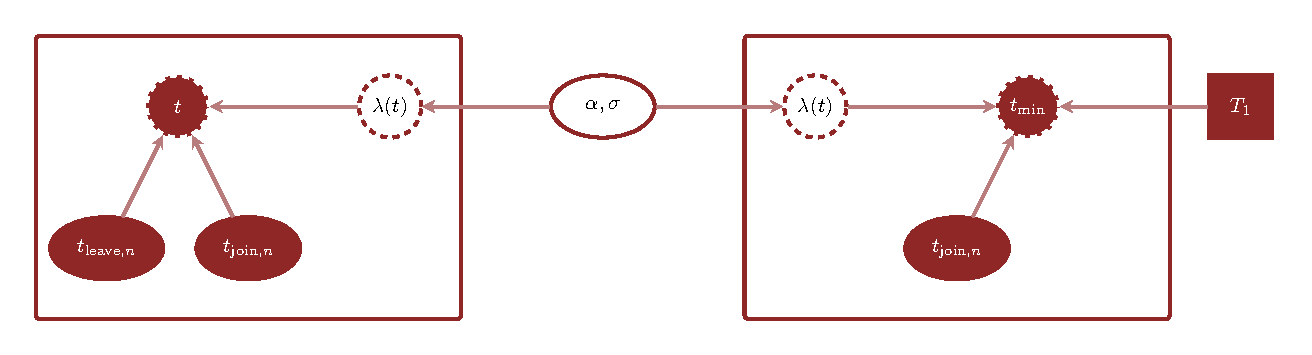
\includegraphics[width=1\textwidth,height=\textheight]{figures/dgms/model3/model3.pdf}

}

\caption{\label{fig-model3}Moving from a constant to a power stimulus
model changes the derived time-to-event model, but not the overall
structure of the data generating process.}

\end{figure}%

\begin{codelisting}

\caption{\texttt{model3.stan}}

\begin{Shaded}
\begin{Highlighting}[]
\KeywordTok{functions}\NormalTok{ \{}
  \CommentTok{// Log stimulus function}
  \DataTypeTok{real}\NormalTok{ log\_lambda(}\DataTypeTok{real}\NormalTok{ t, }\DataTypeTok{real}\NormalTok{ alpha, }\DataTypeTok{real}\NormalTok{ sigma) \{}
    \ControlFlowTok{return}\NormalTok{ log(alpha) {-} log(sigma) + (alpha {-} }\DecValTok{1}\NormalTok{) * log(t / sigma);}
\NormalTok{  \}}
  
  \CommentTok{// Cumulative stimulus function}
  \DataTypeTok{real}\NormalTok{ Lambda(}\DataTypeTok{real}\NormalTok{ t, }\DataTypeTok{real}\NormalTok{ alpha, }\DataTypeTok{real}\NormalTok{ sigma) \{}
    \ControlFlowTok{return}\NormalTok{ pow(t / sigma, alpha);}
\NormalTok{  \}}

  \CommentTok{// Log survival function}
  \DataTypeTok{real}\NormalTok{ log\_survival(}\DataTypeTok{real}\NormalTok{ t, }\DataTypeTok{real}\NormalTok{ alpha, }\DataTypeTok{real}\NormalTok{ sigma) \{}
    \ControlFlowTok{return}\NormalTok{ {-}Lambda(t, alpha, sigma);}
\NormalTok{  \}}

  \CommentTok{// Inverse cumulative stimulus function}
  \DataTypeTok{real}\NormalTok{ Lambda\_inv(}\DataTypeTok{real}\NormalTok{ l, }\DataTypeTok{real}\NormalTok{ alpha, }\DataTypeTok{real}\NormalTok{ sigma) \{}
    \ControlFlowTok{return}\NormalTok{ sigma * pow(l, }\DecValTok{1}\NormalTok{ / alpha);}
\NormalTok{  \}}
  
  \CommentTok{// Inverse survival function}
  \DataTypeTok{real}\NormalTok{ inv\_survival(}\DataTypeTok{real}\NormalTok{ u, }\DataTypeTok{real}\NormalTok{ alpha, }\DataTypeTok{real}\NormalTok{ sigma) \{}
    \ControlFlowTok{return}\NormalTok{ Lambda\_inv({-}log(u), alpha, sigma);}
\NormalTok{  \}}
\NormalTok{\}}

\KeywordTok{data}\NormalTok{ \{}
  \DataTypeTok{real}\NormalTok{           T0; }\CommentTok{// Months}
  \DataTypeTok{real}\NormalTok{\textless{}}\KeywordTok{lower}\NormalTok{=T0\textgreater{} T1; }\CommentTok{// Months}

  \CommentTok{// Churned customers}
  \DataTypeTok{int}\NormalTok{\textless{}}\KeywordTok{lower}\NormalTok{=}\DecValTok{0}\NormalTok{\textgreater{} N\_churn;}
  \DataTypeTok{array}\NormalTok{[N\_churn] }\DataTypeTok{real}\NormalTok{\textless{}}\KeywordTok{lower}\NormalTok{=T0, }\KeywordTok{upper}\NormalTok{=T1\textgreater{} t\_join\_churn;  }\CommentTok{// Months}
  \DataTypeTok{array}\NormalTok{[N\_churn] }\DataTypeTok{real}\NormalTok{\textless{}}\KeywordTok{lower}\NormalTok{=T0, }\KeywordTok{upper}\NormalTok{=T1\textgreater{} t\_leave\_churn; }\CommentTok{// Months}

  \CommentTok{// Active customers}
  \DataTypeTok{int}\NormalTok{\textless{}}\KeywordTok{lower}\NormalTok{=}\DecValTok{0}\NormalTok{\textgreater{} N\_active;}
  \DataTypeTok{array}\NormalTok{[N\_active] }\DataTypeTok{real}\NormalTok{\textless{}}\KeywordTok{lower}\NormalTok{=T0, }\KeywordTok{upper}\NormalTok{=T1\textgreater{} t\_join\_active; }\CommentTok{// Months}
\NormalTok{\}}

\KeywordTok{parameters}\NormalTok{ \{}
  \DataTypeTok{real}\NormalTok{\textless{}}\KeywordTok{lower}\NormalTok{=}\DecValTok{0}\NormalTok{\textgreater{} omega; }\CommentTok{// Inverse shape parameter (Unitless)}
  \DataTypeTok{real}\NormalTok{\textless{}}\KeywordTok{lower}\NormalTok{=}\DecValTok{0}\NormalTok{\textgreater{} sigma; }\CommentTok{// Scale parameter (Months)}
\NormalTok{\}}

\KeywordTok{transformed parameters}\NormalTok{ \{}
  \DataTypeTok{real}\NormalTok{\textless{}}\KeywordTok{lower}\NormalTok{=}\DecValTok{0}\NormalTok{\textgreater{} alpha = }\DecValTok{1}\NormalTok{ / omega;}
\NormalTok{\}}

\KeywordTok{model}\NormalTok{ \{}
  \CommentTok{// Prior Model}
  \CommentTok{// 0 \textless{}\textasciitilde{} omega \textless{}\textasciitilde{} 1}
  \KeywordTok{target +=}\NormalTok{ normal\_lpdf(omega | }\DecValTok{0}\NormalTok{, }\DecValTok{1}\NormalTok{ / }\FloatTok{2.57}\NormalTok{);}

  \CommentTok{// 0 \textless{}\textasciitilde{} sigma \textless{}\textasciitilde{} 75}
  \KeywordTok{target +=}\NormalTok{ normal\_lpdf(sigma | }\DecValTok{0}\NormalTok{, }\DecValTok{75}\NormalTok{ / }\FloatTok{2.57}\NormalTok{);}

  \CommentTok{// Observational Model}
  \ControlFlowTok{for}\NormalTok{ (n }\ControlFlowTok{in} \DecValTok{1}\NormalTok{:N\_churn) \{}
    \DataTypeTok{real}\NormalTok{ tenure = t\_leave\_churn[n] {-} t\_join\_churn[n];}
    \KeywordTok{target +=}\NormalTok{   log\_lambda(tenure, alpha, sigma)}
\NormalTok{              + log\_survival(tenure, alpha, sigma);}
\NormalTok{  \}}

  \ControlFlowTok{for}\NormalTok{ (n }\ControlFlowTok{in} \DecValTok{1}\NormalTok{:N\_active) \{}
    \KeywordTok{target +=}\NormalTok{ log\_survival(T1 {-} t\_join\_active[n], alpha, sigma);}
\NormalTok{  \}}
\NormalTok{\}}

\KeywordTok{generated quantities}\NormalTok{ \{}
  \DataTypeTok{array}\NormalTok{[N\_churn] }\DataTypeTok{real}\NormalTok{\textless{}}\KeywordTok{lower}\NormalTok{=}\DecValTok{0}\NormalTok{\textgreater{} tenure\_churn\_pred;}
  \DataTypeTok{array}\NormalTok{[N\_churn] }\DataTypeTok{real}\NormalTok{\textless{}}\KeywordTok{lower}\NormalTok{=T0\textgreater{} t\_leave\_churn\_pred;}

  \ControlFlowTok{for}\NormalTok{ (n }\ControlFlowTok{in} \DecValTok{1}\NormalTok{:N\_churn) \{}
    \DataTypeTok{real}\NormalTok{ S = exp(log\_survival(T1 {-} t\_join\_churn[n],}
\NormalTok{                              alpha, sigma));}
    \DataTypeTok{real}\NormalTok{ u = uniform\_rng(S, }\DecValTok{1}\NormalTok{);}
\NormalTok{    tenure\_churn\_pred[n]}
\NormalTok{      = inv\_survival(u, alpha, sigma);}
\NormalTok{    t\_leave\_churn\_pred[n]}
\NormalTok{      = t\_join\_churn[n] + tenure\_churn\_pred[n];}
\NormalTok{  \}}
\NormalTok{\}}
\end{Highlighting}
\end{Shaded}

\end{codelisting}

\begin{Shaded}
\begin{Highlighting}[]
\ControlFlowTok{with} \BuiltInTok{open}\NormalTok{(}\StringTok{\textquotesingle{}stan\_programs/model3.stan\textquotesingle{}}\NormalTok{, }\StringTok{\textquotesingle{}r\textquotesingle{}}\NormalTok{) }\ImportTok{as} \BuiltInTok{file}\NormalTok{:}
\NormalTok{  stan\_program }\OperatorTok{=} \BuiltInTok{file}\NormalTok{.read()}
\NormalTok{model }\OperatorTok{=}\NormalTok{ stan.build(stan\_program,}
\NormalTok{                   random\_seed}\OperatorTok{=}\DecValTok{8438338}\NormalTok{,}
\NormalTok{                   data}\OperatorTok{=}\NormalTok{stan\_data)}
\NormalTok{fit }\OperatorTok{=}\NormalTok{ model.sample(num\_samples}\OperatorTok{=}\DecValTok{1024}\NormalTok{, refresh}\OperatorTok{=}\DecValTok{0}\NormalTok{)}
\end{Highlighting}
\end{Shaded}

\begin{verbatim}
Building...
\end{verbatim}

Conveniently, the posterior computation remains well-behaved.

\begin{Shaded}
\begin{Highlighting}[]
\NormalTok{diagnostics }\OperatorTok{=}\NormalTok{ util.extract\_hmc\_diagnostics(fit)}
\NormalTok{util.check\_all\_hmc\_diagnostics(diagnostics)}

\NormalTok{samples }\OperatorTok{=}\NormalTok{ util.extract\_expectand\_vals(fit)}
\NormalTok{base\_samples }\OperatorTok{=}\NormalTok{ util.filter\_expectands(samples,}
\NormalTok{                                      [}\StringTok{\textquotesingle{}omega\textquotesingle{}}\NormalTok{, }\StringTok{\textquotesingle{}sigma\textquotesingle{}}\NormalTok{])}
\NormalTok{util.check\_all\_expectand\_diagnostics(base\_samples)}
\end{Highlighting}
\end{Shaded}

\begin{verbatim}
All Hamiltonian Monte Carlo diagnostics are consistent with accurate
Markov chain Monte Carlo.
 
All expectands checked appear to be behaving well enough for reliable
Markov chain Monte Carlo estimation.
 
\end{verbatim}

\subsection{Posterior Retrodictive
Checks}\label{posterior-retrodictive-checks-2}

Overall, the retrodictive agreement for both the tenure and leave times
has improved quite a bit. That said, the agreement still leaves
something to be desired.

\begin{Shaded}
\begin{Highlighting}[]
\NormalTok{f, axarr }\OperatorTok{=}\NormalTok{ plot.subplots(}\DecValTok{2}\NormalTok{, }\DecValTok{1}\NormalTok{, layout}\OperatorTok{=}\StringTok{"constrained"}\NormalTok{)}

\NormalTok{putil.plot\_hist\_quantiles(}
\NormalTok{  axarr[}\DecValTok{0}\NormalTok{], samples, }\StringTok{\textquotesingle{}tenure\_churn\_pred\textquotesingle{}}\NormalTok{,}
\NormalTok{  data[}\StringTok{\textquotesingle{}T0\textquotesingle{}}\NormalTok{] }\OperatorTok{{-}} \DecValTok{1}\NormalTok{, data[}\StringTok{\textquotesingle{}T1\textquotesingle{}}\NormalTok{] }\OperatorTok{+} \DecValTok{1}\NormalTok{, }\DecValTok{1}\NormalTok{,}
\NormalTok{  baseline\_values}\OperatorTok{=}\NormalTok{tenure\_churn,}
\NormalTok{  xlabel}\OperatorTok{=}\StringTok{\textquotesingle{}Customer Tenure (months)\textquotesingle{}}
\NormalTok{)}


\NormalTok{putil.plot\_hist\_quantiles(}
\NormalTok{  axarr[}\DecValTok{1}\NormalTok{], samples, }\StringTok{\textquotesingle{}t\_leave\_churn\_pred\textquotesingle{}}\NormalTok{,}
\NormalTok{  data[}\StringTok{\textquotesingle{}T0\textquotesingle{}}\NormalTok{] }\OperatorTok{{-}} \DecValTok{3}\NormalTok{, data[}\StringTok{\textquotesingle{}T1\textquotesingle{}}\NormalTok{] }\OperatorTok{+} \DecValTok{23}\NormalTok{, }\DecValTok{3}\NormalTok{,}
\NormalTok{  baseline\_values}\OperatorTok{=}\NormalTok{data[}\StringTok{\textquotesingle{}t\_leave\_churn\textquotesingle{}}\NormalTok{],}
\NormalTok{  xlabel}\OperatorTok{=}\StringTok{"Time Customer Leaves (months)"}
\NormalTok{)}
\NormalTok{axarr[}\DecValTok{1}\NormalTok{].axvline(x}\OperatorTok{=}\NormalTok{data[}\StringTok{\textquotesingle{}T0\textquotesingle{}}\NormalTok{], linewidth}\OperatorTok{=}\DecValTok{2}\NormalTok{,}
\NormalTok{                 linestyle}\OperatorTok{=}\StringTok{\textquotesingle{}dashed\textquotesingle{}}\NormalTok{, color}\OperatorTok{=}\StringTok{"\#DDDDDD"}\NormalTok{)}
\NormalTok{axarr[}\DecValTok{1}\NormalTok{].axvline(x}\OperatorTok{=}\NormalTok{data[}\StringTok{\textquotesingle{}T1\textquotesingle{}}\NormalTok{], linewidth}\OperatorTok{=}\DecValTok{2}\NormalTok{,}
\NormalTok{                 linestyle}\OperatorTok{=}\StringTok{\textquotesingle{}dashed\textquotesingle{}}\NormalTok{, color}\OperatorTok{=}\StringTok{"\#DDDDDD"}\NormalTok{)}

\NormalTok{plot.show()}
\end{Highlighting}
\end{Shaded}

\includegraphics{churn_files/figure-pdf/cell-38-output-1.png}

This residual tension isn't necessarily surprising. Remember that we
have yet to consider demographic heterogeneity! Indeed, when we examine
the binned medians, we see strong disagreement between the posterior
predictions and the observed data.

\begin{Shaded}
\begin{Highlighting}[]
\NormalTok{bin\_min }\OperatorTok{=}\NormalTok{ [ }\DecValTok{0}\NormalTok{, }\DecValTok{0}\NormalTok{, }\DecValTok{0}\NormalTok{, }\DecValTok{0}\NormalTok{ ]}
\NormalTok{bin\_max }\OperatorTok{=}\NormalTok{ [ }\DecValTok{100}\NormalTok{, }\DecValTok{15}\NormalTok{, }\FloatTok{1.05}\NormalTok{, }\DecValTok{1000}\NormalTok{ ]}
\NormalTok{bin\_delta }\OperatorTok{=}\NormalTok{ [ }\DecValTok{20}\NormalTok{, }\DecValTok{1}\NormalTok{, }\FloatTok{0.20}\NormalTok{, }\DecValTok{200}\NormalTok{ ]}

\NormalTok{pred\_names }\OperatorTok{=}\NormalTok{ [ }\SpecialStringTok{f\textquotesingle{}tenure\_churn\_pred[}\SpecialCharTok{\{}\NormalTok{n }\OperatorTok{+} \DecValTok{1}\SpecialCharTok{\}}\SpecialStringTok{]\textquotesingle{}}
               \ControlFlowTok{for}\NormalTok{ n }\KeywordTok{in} \BuiltInTok{range}\NormalTok{(data[}\StringTok{\textquotesingle{}N\_churn\textquotesingle{}}\NormalTok{]) ]}

\NormalTok{f, axarr }\OperatorTok{=}\NormalTok{ plot.subplots(}\DecValTok{2}\NormalTok{, }\DecValTok{2}\NormalTok{, layout}\OperatorTok{=}\StringTok{"constrained"}\NormalTok{)}

\ControlFlowTok{for}\NormalTok{ i }\KeywordTok{in} \BuiltInTok{range}\NormalTok{(data[}\StringTok{\textquotesingle{}I\textquotesingle{}}\NormalTok{]):}
\NormalTok{  i1 }\OperatorTok{=}\NormalTok{ i }\OperatorTok{//} \DecValTok{2}
\NormalTok{  i2 }\OperatorTok{=}\NormalTok{ i }\OperatorTok{\%} \DecValTok{2}

\NormalTok{  putil.plot\_conditional\_median\_quantiles(}
\NormalTok{    axarr[i1, i2], samples, pred\_names,}
\NormalTok{    [ x[i] }\ControlFlowTok{for}\NormalTok{ x }\KeywordTok{in}\NormalTok{ data[}\StringTok{\textquotesingle{}X\_churn\textquotesingle{}}\NormalTok{] ],}
\NormalTok{    bin\_min[i], bin\_max[i], bin\_delta[i],}
\NormalTok{    tenure\_churn, residual}\OperatorTok{=}\VariableTok{False}\NormalTok{,}
\NormalTok{    xlabel}\OperatorTok{=}\NormalTok{data[}\StringTok{\textquotesingle{}x\_names\textquotesingle{}}\NormalTok{][i], ylabel}\OperatorTok{=}\StringTok{""}
\NormalTok{  )}

\NormalTok{plot.show()}
\end{Highlighting}
\end{Shaded}

\begin{verbatim}
1 conditioning values (0.04%) fell below the histogram binning.
6 conditioning values (0.27%) fell above the histogram binning.
\end{verbatim}

\includegraphics{churn_files/figure-pdf/cell-39-output-2.png}

\section{Model 4: Power Stimulus/Hazard Model with Censoring and
Proportional
Stimuli/Hazards}\label{model-4-power-stimulushazard-model-with-censoring-and-proportional-stimulihazards}

In order to improve our model, we have to address a question that is
easy to take for granted but is often diabolically subtle. Exactly what
behaviors could vary with the available demographic variables?

\subsection{Observational Model}\label{observational-model-2}

Instead of considering which features of the time-to-event model can
vary with external variables, the \emph{proportional stimulus model}
allows the external variables to scale the underlying stimulus function.
This dependence then propagates to the derived time-to-event model.

The precise coupling between the stimulus function behavior and the
demographic variables is not always static; it can generally vary with
the behavior of the demographic variables. In the language of regression
modeling, the conditional relationship between event time and the
demographic variables can be
\href{http://www.symplectomorphic.com/assets/case_studies/variate_covariate_modeling.html}{confounded}
with the marginal behavior of the external variables.

Here we will assume that any confounding is negligible, so that we can
safely ignore the latter. That said, this is a strong assumption that
has to be justified from domain expertise in a real analysis.

If we denote the continuous demographic variables for the \(n\)th
customer as \[
(x_{n1}, \ldots, x_{nI})
\] and the categorical demographic variables as \[
(l^{1}_{n}, \ldots, l^{K}_{n}),
\] then the proportional stimulus model can be written as \[
\lambda(t)
=
\lambda_{0}(t) \, \exp (
  f(
    x_{n1}, \ldots, x_{nI},
    \nu^{1}_{l^{1}_{n}}, \ldots, \nu^{K}_{l^{K}_{n}}
   )
)
\] To ensure that the survival model is well-behaved, the outputs of the
function \(f\) must be positive.

The baseline stimulus function \(\lambda_{0}(t)\) models the behavior
for the implicit baseline configuration satisfying \[
f(x_{n1}, \ldots, x_{nI},
  \nu^{1}_{l^{1}_{n}}, \ldots, \nu^{K}_{l^{K}_{n}},
) = 1.
\] If the output of \(f\) is smaller than one, then it suppresses the
driving stimulation, leading to later event times. When the output is
larger than one, the stimulus is amplified and event times accelerate.
The precise form of \(f\) determines exactly how customer tenure varies
as the demographic variables deviate from the implicit baseline.

There is no end of possible function models that we might consider.
Proportional stimulus models, however, almost always assume an
exponential-linear functional form, \[
\lambda(t)
=
\lambda_{0}(t) \,
\exp \left(
    \sum_{i = 1}^{I} \beta_{i} \, (x_{ni} - x_{0i})
  + \sum_{k = 1}^{K} \delta^{k}_{l^{k}_{n}}
\right),
\] where \[
\delta^{k}_{l^{k}_{n}}
=
\nu^{k}_{l^{k}_{n}}
-
\nu^{k}_{l^{k}_{0}}.
\]

We can always interpret this exponential-linear model as a local
\href{http://www.symplectomorphic.com/assets/case_studies/general_taylor_models.html}{approximation}
to a nonlinear functional model around a baseline configuration of the
demographic variables. Conveniently, the configuration for this
functional model is explicitly given by \(x_{ni} = x_{0i}\) and
\(l^{k}_{n} = l^{k}_{0}\).

Given this functional model, the complete proportional power stimulus
function is given by \[
\lambda(t)
=
\alpha \, \frac{1}{\sigma} \,
\left( \frac{t}{\sigma} \right)^{\alpha - 1} \,
\exp \left(
    \sum_{i = 1}^{I} \beta_{i} \, (x_{ni} - x_{0i})
  + \sum_{k = 1}^{K} \delta^{k}_{l^{k}_{n}}
\right)
\] with the resulting cumulative stimulus function \[
\Lambda(t)
=
\left( \frac{t}{\sigma} \right)^{\alpha} \,
\exp \left(
    \sum_{i = 1}^{I} \beta_{i} \, (x_{ni} - x_{0i})
  + \sum_{k = 1}^{K} \delta^{k}_{l^{k}_{n}}
\right),
\] and survival function \[
S(t)
=
\exp \left(
  - \left( \frac{t}{\sigma} \right)^{\alpha} \,
    \exp \left(
        \sum_{i = 1}^{I} \beta_{i} \, (x_{ni} - x_{0i})
      + \sum_{k = 1}^{K} \delta^{k}_{l^{k}_{n}}
    \right)
\right).
\]

The time-to-event model then becomes \begin{align*}
p(t)
&=\;
\alpha \, \frac{1}{\sigma} \,
\left( \frac{t}{\sigma} \right)^{\alpha - 1} \,
\\
&\quad \cdot
\exp \left(
    \sum_{i = 1}^{I} \beta_{i} \, (x_{ni} - x_{0i})
  + \sum_{k = 1}^{K} \delta^{k}_{l^{k}_{n}}
\right) \,
\\
&\quad \cdot
\exp \left(
  - \left( \frac{t}{\sigma} \right)^{\alpha} \,
    \exp \left(
        \sum_{i = 1}^{I} \beta_{i} \, (x_{ni} - x_{0i})
      + \sum_{k = 1}^{K} \delta^{k}_{l^{k}_{n}}
    \right)
\right)
\\
&=
\alpha \, \frac{1}{\tau} \,
\left( \frac{t}{\tau} \right)^{\alpha - 1} \,
\exp \left(
  - \left( \frac{t}{\tau} \right)^{\alpha} \,
\right)
\\
&=
\mathrm{weibull}(t \mid \alpha, \tau)
\end{align*} where \[
\tau
=
\sigma \, \exp \left(
    \sum_{i = 1}^{I} \beta_{i} \, (x_{ni} - x_{0i})
  + \sum_{k = 1}^{K} \delta^{k}_{l^{k}_{n}}
\right)
\]

Coincidentally, only the second parameter of the time-to-event model
varies with the demographic variables in this case. More generally,
multiple if not all of the time-to-event model parameters can vary with
the demographic variables.

\subsection{Transforming the
Covariates}\label{transforming-the-covariates}

One weakness of the exponential-linear model is that is can poorly
approximate functional behavior when the input variables concentrate
near a boundary. Unfortunately, this is exactly the case here for the
observed wealth percentiles and monthly margins. That said, we can often
improve the approximation power of the exponential-linear by first
\href{http://www.symplectomorphic.com/assets/case_studies/taylor_models.html\#14_Covariate_Boundaries}{unconstraining}
these variables.

Allowing each continuous demographic variable to be transformed is
equivalent to the slightly more sophisticated functional model
\begin{align*}
f(
  x_{n1}, &\ldots, x_{nI},
  \nu^{1}_{l^{1}_{n}}, \ldots, \nu^{K}_{l^{K}_{n}}
)
\\
&=
\exp \left(
    \sum_{i = 1}^{I} \beta_{i} \, ( g_{i}(x_{ni}) - g_{i}(x_{0i}) )
  + \sum_{k = 1}^{K} \delta^{k}_{l^{k}_{n}}
\right)
\end{align*} for appropriate transformation functions \(g_{i}\). This,
in turn, is equivalent to using modified demographic variables,
\begin{align*}
f(
  x_{n1}, &\ldots, x_{nI},
  \nu^{1}_{l^{1}_{n}}, \ldots, \nu^{K}_{l^{K}_{n}}
)
\\
&=
\exp \left(
    \sum_{i = 1}^{I} \beta_{i} \, ( g_{i}(x_{ni}) - g_{i}(x_{0i}) )
  + \sum_{k = 1}^{K} \delta^{k}_{l^{k}_{n}}
\right)
\\
&=
\exp \left(
    \sum_{i = 1}^{I} \beta_{i} \, ( z_{ni} - z{0i} )
  + \sum_{k = 1}^{K} \delta^{k}_{l^{k}_{n}}
\right)
\end{align*}

The interval constraints of wealth percentiles can be transformed away
with the logit function, while the positivity constraint of the monthly
margins can be transformed away with the natural logarithm. We'll leave
the observed age and product counts unmodified, as they concentrate
relatively far away from their lower zero boundaries.

\begin{Shaded}
\begin{Highlighting}[]
\KeywordTok{def}\NormalTok{ logit(x):}
  \ControlFlowTok{return}\NormalTok{ math.log(x }\OperatorTok{/}\NormalTok{ (}\DecValTok{1} \OperatorTok{{-}}\NormalTok{ x))}

\KeywordTok{def}\NormalTok{ transform\_covariates(x):}
  \ControlFlowTok{return}\NormalTok{ [ x[}\DecValTok{0}\NormalTok{], x[}\DecValTok{1}\NormalTok{], logit(x[}\DecValTok{2}\NormalTok{]), math.log(x[}\DecValTok{3}\NormalTok{]) ]}

\NormalTok{z\_names }\OperatorTok{=}\NormalTok{ [ data[}\StringTok{\textquotesingle{}x\_names\textquotesingle{}}\NormalTok{][}\DecValTok{0}\NormalTok{],}
\NormalTok{            data[}\StringTok{\textquotesingle{}x\_names\textquotesingle{}}\NormalTok{][}\DecValTok{1}\NormalTok{],}
            \SpecialStringTok{f\textquotesingle{}logit(Wealth / Percentile)\textquotesingle{}}\NormalTok{,}
            \SpecialStringTok{f\textquotesingle{}log(Monthly Margin / Euro)\textquotesingle{}}\NormalTok{    ]}
\end{Highlighting}
\end{Shaded}

\begin{Shaded}
\begin{Highlighting}[]
\NormalTok{Z\_churn }\OperatorTok{=}\NormalTok{ [ transform\_covariates(x)}
            \ControlFlowTok{for}\NormalTok{ x }\KeywordTok{in}\NormalTok{ data[}\StringTok{\textquotesingle{}X\_churn\textquotesingle{}}\NormalTok{] ]}

\NormalTok{Z\_active }\OperatorTok{=}\NormalTok{ [ transform\_covariates(x)}
            \ControlFlowTok{for}\NormalTok{ x }\KeywordTok{in}\NormalTok{ data[}\StringTok{\textquotesingle{}X\_active\textquotesingle{}}\NormalTok{] ]}
\end{Highlighting}
\end{Shaded}

As expected, the transformed demographic variables no longer bunch up at
their lower boundary.

\begin{Shaded}
\begin{Highlighting}[]
\NormalTok{bin\_min }\OperatorTok{=}\NormalTok{ [ }\DecValTok{0}\NormalTok{, }\DecValTok{0}\NormalTok{, }\OperatorTok{{-}}\DecValTok{10}\NormalTok{, }\OperatorTok{{-}}\DecValTok{10}\NormalTok{ ]}
\NormalTok{bin\_max }\OperatorTok{=}\NormalTok{ [ }\DecValTok{100}\NormalTok{, }\DecValTok{10}\NormalTok{, }\DecValTok{10}\NormalTok{, }\DecValTok{10}\NormalTok{ ]}
\NormalTok{bin\_delta }\OperatorTok{=}\NormalTok{ [ }\DecValTok{5}\NormalTok{, }\DecValTok{1}\NormalTok{, }\DecValTok{1}\NormalTok{, }\DecValTok{1}\NormalTok{ ]}

\NormalTok{f, axarr }\OperatorTok{=}\NormalTok{ plot.subplots(}\DecValTok{2}\NormalTok{, }\DecValTok{2}\NormalTok{, layout}\OperatorTok{=}\StringTok{"constrained"}\NormalTok{)}

\ControlFlowTok{for}\NormalTok{ i }\KeywordTok{in} \BuiltInTok{range}\NormalTok{(data[}\StringTok{\textquotesingle{}I\textquotesingle{}}\NormalTok{]):}
\NormalTok{  i1 }\OperatorTok{=}\NormalTok{ i }\OperatorTok{//} \DecValTok{2}
\NormalTok{  i2 }\OperatorTok{=}\NormalTok{ i }\OperatorTok{\%} \DecValTok{2}

\NormalTok{  putil.plot\_line\_hist(axarr[i1, i2],}
\NormalTok{                       [ z[i] }\ControlFlowTok{for}\NormalTok{ z }\KeywordTok{in}\NormalTok{ Z\_churn ],}
\NormalTok{                       bin\_min[i], bin\_max[i], bin\_delta[i],}
\NormalTok{                       xlabel}\OperatorTok{=}\NormalTok{z\_names[i])}
\NormalTok{plot.show()}
\end{Highlighting}
\end{Shaded}

\begin{verbatim}
1 values (0.04%) fell below the histogram binning.
3 values (0.13%) fell above the histogram binning.
18 values (0.80%) fell above the histogram binning.
\end{verbatim}

\includegraphics{churn_files/figure-pdf/cell-42-output-2.png}

Our model recovers customer tenure binned in these transformed
demographic variables just as poorly as it did in bins of the
unprocessed demographic variables.

\begin{Shaded}
\begin{Highlighting}[]
\NormalTok{bin\_min }\OperatorTok{=}\NormalTok{ [ }\DecValTok{0}\NormalTok{, }\DecValTok{0}\NormalTok{, }\OperatorTok{{-}}\DecValTok{10}\NormalTok{, }\OperatorTok{{-}}\DecValTok{10}\NormalTok{ ]}
\NormalTok{bin\_max }\OperatorTok{=}\NormalTok{ [ }\DecValTok{100}\NormalTok{, }\DecValTok{15}\NormalTok{, }\DecValTok{10}\NormalTok{, }\DecValTok{10}\NormalTok{ ]}
\NormalTok{bin\_delta }\OperatorTok{=}\NormalTok{ [ }\DecValTok{10}\NormalTok{, }\DecValTok{1}\NormalTok{, }\DecValTok{2}\NormalTok{, }\DecValTok{2}\NormalTok{ ]}

\NormalTok{pred\_names }\OperatorTok{=}\NormalTok{ [ }\SpecialStringTok{f\textquotesingle{}tenure\_churn\_pred[}\SpecialCharTok{\{}\NormalTok{n }\OperatorTok{+} \DecValTok{1}\SpecialCharTok{\}}\SpecialStringTok{]\textquotesingle{}}
               \ControlFlowTok{for}\NormalTok{ n }\KeywordTok{in} \BuiltInTok{range}\NormalTok{(data[}\StringTok{\textquotesingle{}N\_churn\textquotesingle{}}\NormalTok{]) ]}

\NormalTok{f, axarr }\OperatorTok{=}\NormalTok{ plot.subplots(}\DecValTok{2}\NormalTok{, }\DecValTok{2}\NormalTok{, layout}\OperatorTok{=}\StringTok{"constrained"}\NormalTok{)}

\ControlFlowTok{for}\NormalTok{ i }\KeywordTok{in} \BuiltInTok{range}\NormalTok{(data[}\StringTok{\textquotesingle{}I\textquotesingle{}}\NormalTok{]):}
\NormalTok{  i1 }\OperatorTok{=}\NormalTok{ i }\OperatorTok{//} \DecValTok{2}
\NormalTok{  i2 }\OperatorTok{=}\NormalTok{ i }\OperatorTok{\%} \DecValTok{2}

\NormalTok{  putil.plot\_conditional\_median\_quantiles(}
\NormalTok{    axarr[i1, i2], samples, pred\_names,}
\NormalTok{    [ z[i] }\ControlFlowTok{for}\NormalTok{ z }\KeywordTok{in}\NormalTok{ Z\_churn ],}
\NormalTok{    bin\_min[i], bin\_max[i], bin\_delta[i],}
\NormalTok{    tenure\_churn, residual}\OperatorTok{=}\VariableTok{False}\NormalTok{,}
\NormalTok{    xlabel}\OperatorTok{=}\NormalTok{z\_names[i], ylabel}\OperatorTok{=}\StringTok{""}
\NormalTok{  )}

\NormalTok{plot.show()}
\end{Highlighting}
\end{Shaded}

\begin{verbatim}
1 conditioning values (0.04%) fell below the histogram binning.
18 conditioning values (0.80%) fell above the histogram binning.
\end{verbatim}

\includegraphics{churn_files/figure-pdf/cell-43-output-2.png}

\subsection{Demographic Baseline}\label{demographic-baseline}

All that's left is to specify a baseline configuration of the
demographic variables. This baseline effectively defines a default
customer, relative to whom we can interpret the demographic
heterogeneity. Note that this default customer can be completely
hypothetical, and does not have to correspond to any particular observed
customer.

We'll take the baseline online banking configuration to be false.
Because online banking features only two categories, true and false, we
can implement this contribution by adding a single parameter
\(\delta_{\mathrm{online}}\) for when a customer participates in online
banking.

This leaves the continuous demographic variables.

\begin{Shaded}
\begin{Highlighting}[]
\NormalTok{x0 }\OperatorTok{=}\NormalTok{ [}
 \DecValTok{40}\NormalTok{,  }\CommentTok{\# Age (years)}
 \DecValTok{2}\NormalTok{,   }\CommentTok{\# Number of bank products (counts)}
 \FloatTok{0.5}\NormalTok{, }\CommentTok{\# Wealth (Percentile)}
 \DecValTok{50}   \CommentTok{\# Monthly Margin (euros)}
\NormalTok{]}
\end{Highlighting}
\end{Shaded}

To use this baseline configuration in our model, however, we'll need to
apply the appropriate transformations.

\begin{Shaded}
\begin{Highlighting}[]
\NormalTok{z0 }\OperatorTok{=}\NormalTok{ transform\_covariates(x0)}

\NormalTok{stan\_data[}\StringTok{\textquotesingle{}z0\textquotesingle{}}\NormalTok{] }\OperatorTok{=}\NormalTok{ z0}
\NormalTok{stan\_data[}\StringTok{\textquotesingle{}Z\_churn\textquotesingle{}}\NormalTok{] }\OperatorTok{=}\NormalTok{ Z\_churn}
\NormalTok{stan\_data[}\StringTok{\textquotesingle{}Z\_active\textquotesingle{}}\NormalTok{] }\OperatorTok{=}\NormalTok{ Z\_active}
\end{Highlighting}
\end{Shaded}

\subsection{Prior Model}\label{prior-model-2}

One benefit of the proportional stimulus model is that we can motivate
an informative prior model for the new parameters by reasoning about
thresholds in proportional changes.

Consider, for example, a categorical demographic variable. If the value
of \emph{only} this variable changes from its baseline to
\(\delta^{k}_{l}\), then the stimulus function is proportionally scaled
by \(\exp( \delta^{k}_{l} )\). Consequently, constraining the reasonable
proportional variations constrains reasonable values for
\(\delta^{k}_{l}\), \begin{align*}
\frac{1}{\delta} &\lessapprox
\exp( \delta^{k}_{l} ) \lessapprox
\delta
\\
- \log \delta &\lessapprox
\delta^{k}_{l} \lessapprox
+ \log \delta
\end{align*}

For online banking participation, we'll take \(\delta = 5\) so that \[
\vert \delta_{\mathrm{online}} \vert < \log 5.
\] Note that \(500\%\) is an absolutely huge proportional change; this
prior model is \emph{extremely} weakly informative relative to what
domain expertise would be available in most applications!

To motivate prior models for coefficients of the remaining demographic
variables, we can consider constraining the proportional variation when
each component individually deviates from its baseline by a certain
amount, \begin{align*}
\frac{1}{\delta} &\lessapprox
\exp( \beta_{i} \, \Delta x_{i} ) \lessapprox
\delta
\\
- \log \delta &\lessapprox
\beta_{i} \, \Delta x_{i} \lessapprox
+ \log \delta
\\
- \frac{ \log \delta}{ \Delta x_{i} } &\lessapprox
\beta_{i} \lessapprox
+ \frac{ \log \delta }{ \Delta x_{i} }
\end{align*}

For age we'll take \(\delta = 5\) and \(\Delta x_{i} = 10\) so that \[
\vert \beta_{\mathrm{age}} \vert < \frac{ \log 5 }{ 10 },
\] while for the number of banking products we'll take \(\delta = 5\)
and \(\Delta x_{i} = 1\) so that \[
\vert \beta_{\mathrm{products}} \vert < \frac{ \log 5 }{ 1 }.
\]

When working with the transformed demographic variables, however, we'll
want to take those transformations into account. For example, log
transforming a demographic variable is equivalent to the proportional
variation \begin{align*}
\exp \left( \beta_{i} \, (\log x_{i} - \log x_{0i}) \right)
&=
\exp \left( \beta_{i} \, \log \frac{ x_{i} }{ x_{0i} } \right)
\\
&=
\exp \left(
  \log \left( \frac{ x_{i} }{ x_{0i} } \right)^{\beta_{i}}
\right)
\\
&=
\left( \frac{ x_{i} }{ x_{0i} } \right)^{\beta_{i}}
\end{align*}

Consequently, the corresponding prior model is informed by reasoning
about proportional output variation given proportional input variation.
If \[
x_{i} = \zeta \, x_{0i}
\] then \begin{align*}
\frac{1}{\delta} &\lessapprox
\bigg( \frac{ x_{i} }{ x_{0i} } \bigg)^{\beta_{i}} \lessapprox
\delta
\\
\frac{1}{\delta} &\lessapprox
\bigg( \zeta \bigg)^{\beta_{i}} \lessapprox
\delta
\\
- \log \delta &\lessapprox
\beta_{i} \, \log\zeta \lessapprox
+ \log \delta
\\
- \frac{ \log \delta }{ \log \zeta } &\lessapprox
\beta_{i} \lessapprox
+ \frac{ \log \delta }{ \log \zeta}.
\end{align*}

For monthly margin we'll take \(\delta = 5\) and \(\zeta = 2\) so that
\[
\vert \beta_{i} \vert < \frac{ \log 5 }{ \log 2}.
\]

Accounting for logit transformed demographic variables is a bit more
subtle. First we have \begin{align*}
\exp \left(
  \beta_{i} \, (\mathrm{logit} x_{i} - \mathrm{logit} x_{0i})
\right)
&=
\exp \left(
  \beta_{i} \, \left(
      \log \frac{ x_{i} }{ 1 - x_{i} }
    - \log \frac{ x_{0i} }{ 1 - x_{0i} }
  \right)
\right)
\\
&=
\exp \left(
  \beta_{i} \,
  \log \left(
    \frac{ x_{i} }{ 1 - x_{i} } \frac{ 1 - x_{0i} }{ x_{0i} }
  \right)
\right)
\\
&=
\exp \left(
  \log \left(
    \frac{ x_{i} }{ 1 - x_{i} } \frac{ 1 - x_{0i} }{ x_{0i} }
  \right)^{\beta_{i}}
\right)
\\
&=
\left(
  \frac{ x_{i} }{ 1 - x_{i} } \frac{ 1 - x_{0i} }{ x_{0i} }
\right)^{\beta_{i}}
\end{align*}

In this case, we need to think about how the proportional output changes
given proportional changes in the input \emph{odds}, \[
\zeta
=
\frac{ x_{i} }{ 1 - x_{i} } \frac{ 1 - x_{0i} }{ x_{0i} }.
\] This gives \[
- \frac{ \log \delta }{ \log \zeta } \lessapprox
\beta_{i} \lessapprox
+ \frac{ \log \delta }{ \log \zeta}.
\]

For wealth percentile we'll take \(\delta = 5\) and \(\zeta = 2\) so
that \[
\vert \beta_{i} \vert < \frac{ \log 5 }{ \log 2}.
\]

We don't want any unexpected interaction between the demographic
variables to spoil our careful prior model development. Specifically, we
should be diligent and perform a prior check.

\begin{codelisting}

\caption{\texttt{model4\textbackslash\_prior.stan}}

\begin{Shaded}
\begin{Highlighting}[]
\KeywordTok{functions}\NormalTok{ \{}
  \CommentTok{// Log stimulus function}
  \DataTypeTok{real}\NormalTok{ log\_lambda(}\DataTypeTok{real}\NormalTok{ t, }\DataTypeTok{real}\NormalTok{ alpha, }\DataTypeTok{real}\NormalTok{ sigma) \{}
    \ControlFlowTok{return}\NormalTok{ log(alpha) {-} log(sigma) + (alpha {-} }\DecValTok{1}\NormalTok{) * log(t / sigma);}
\NormalTok{  \}}
  
  \CommentTok{// Cumulative stimulus function}
  \DataTypeTok{real}\NormalTok{ Lambda(}\DataTypeTok{real}\NormalTok{ t, }\DataTypeTok{real}\NormalTok{ alpha, }\DataTypeTok{real}\NormalTok{ sigma) \{}
    \ControlFlowTok{return}\NormalTok{ pow(t / sigma, alpha);}
\NormalTok{  \}}

  \CommentTok{// Log survival function}
  \DataTypeTok{real}\NormalTok{ log\_survival(}\DataTypeTok{real}\NormalTok{ t, }\DataTypeTok{real}\NormalTok{ alpha, }\DataTypeTok{real}\NormalTok{ sigma) \{}
    \ControlFlowTok{return}\NormalTok{ {-}Lambda(t, alpha, sigma);}
\NormalTok{  \}}

  \CommentTok{// Inverse cumulative stimulus function}
  \DataTypeTok{real}\NormalTok{ Lambda\_inv(}\DataTypeTok{real}\NormalTok{ l, }\DataTypeTok{real}\NormalTok{ alpha, }\DataTypeTok{real}\NormalTok{ sigma) \{}
    \ControlFlowTok{return}\NormalTok{ sigma * pow(l, }\DecValTok{1}\NormalTok{ / alpha);}
\NormalTok{  \}}
  
  \CommentTok{// Inverse survival function}
  \DataTypeTok{real}\NormalTok{ inv\_survival(}\DataTypeTok{real}\NormalTok{ u, }\DataTypeTok{real}\NormalTok{ alpha, }\DataTypeTok{real}\NormalTok{ sigma) \{}
    \ControlFlowTok{return}\NormalTok{ Lambda\_inv({-}log(u), alpha, sigma);}
\NormalTok{  \}}
\NormalTok{\}}

\KeywordTok{data}\NormalTok{ \{}
  \DataTypeTok{real}\NormalTok{\textless{}}\KeywordTok{lower}\NormalTok{=}\DecValTok{0}\NormalTok{\textgreater{} t\_lower;}
  \DataTypeTok{real}\NormalTok{\textless{}}\KeywordTok{lower}\NormalTok{=}\DecValTok{0}\NormalTok{\textgreater{} t\_upper;}

  \DataTypeTok{int}\NormalTok{ I;            }\CommentTok{// Number of covariates}
  \DataTypeTok{row\_vector}\NormalTok{[I] z0; }\CommentTok{// Covariate baselines}

  \CommentTok{// Churned customers}
  \DataTypeTok{int}\NormalTok{\textless{}}\KeywordTok{lower}\NormalTok{=}\DecValTok{0}\NormalTok{\textgreater{} N\_churn;}
  \DataTypeTok{matrix}\NormalTok{[N\_churn, I] Z\_churn;}
  \DataTypeTok{array}\NormalTok{[N\_churn] }\DataTypeTok{int}\NormalTok{ online\_banking\_churn;}
\NormalTok{\}}

\KeywordTok{parameters}\NormalTok{ \{}
  \DataTypeTok{real}\NormalTok{\textless{}}\KeywordTok{lower}\NormalTok{=}\DecValTok{0}\NormalTok{\textgreater{} omega; }\CommentTok{// Inverse shape parameter (Unitless)}
  \DataTypeTok{real}\NormalTok{\textless{}}\KeywordTok{lower}\NormalTok{=}\DecValTok{0}\NormalTok{\textgreater{} sigma; }\CommentTok{// Scale parameter (Months)}

  \DataTypeTok{vector}\NormalTok{[I] beta;    }\CommentTok{// Covariate slopes (1 / covariate units)}
  \DataTypeTok{real}\NormalTok{ delta\_online; }\CommentTok{// Online banking contribution}
\NormalTok{\}}

\KeywordTok{transformed parameters}\NormalTok{ \{}
  \DataTypeTok{real}\NormalTok{\textless{}}\KeywordTok{lower}\NormalTok{=}\DecValTok{0}\NormalTok{\textgreater{} alpha = }\DecValTok{1}\NormalTok{ / omega;}
\NormalTok{\}}

\KeywordTok{model}\NormalTok{ \{}
  \CommentTok{// Prior Model}
  \CommentTok{// 0 \textless{}\textasciitilde{} omega \textless{}\textasciitilde{} 1}
  \KeywordTok{target +=}\NormalTok{ normal\_lpdf(omega | }\DecValTok{0}\NormalTok{, }\DecValTok{1}\NormalTok{ / }\FloatTok{2.57}\NormalTok{);}

  \CommentTok{// 0 \textless{}\textasciitilde{} sigma \textless{}\textasciitilde{} 75}
  \KeywordTok{target +=}\NormalTok{ normal\_lpdf(sigma | }\DecValTok{0}\NormalTok{, }\DecValTok{75}\NormalTok{ / }\FloatTok{2.57}\NormalTok{);}

  \CommentTok{// {-}log(5) / 10 \textless{}\textasciitilde{} beta[1] \textless{}\textasciitilde{} +log(5) / 10}
  \KeywordTok{target +=}\NormalTok{ normal\_lpdf(beta[}\DecValTok{1}\NormalTok{] | }\DecValTok{0}\NormalTok{, }\FloatTok{0.07}\NormalTok{);}

  \CommentTok{// {-}log(5) / 1 \textless{}\textasciitilde{} beta[2] \textless{}\textasciitilde{} +log(5) / 1}
  \KeywordTok{target +=}\NormalTok{ normal\_lpdf(beta[}\DecValTok{2}\NormalTok{] | }\DecValTok{0}\NormalTok{, }\FloatTok{0.70}\NormalTok{);}

  \CommentTok{// {-}log(5) / 2 \textless{}\textasciitilde{} beta[3] \textless{}\textasciitilde{} +log(5) / 2}
  \KeywordTok{target +=}\NormalTok{ normal\_lpdf(beta[}\DecValTok{3}\NormalTok{] | }\DecValTok{0}\NormalTok{, }\FloatTok{0.35}\NormalTok{);}

  \CommentTok{// {-}log(5) / log(2) \textless{}\textasciitilde{} beta[4] \textless{}\textasciitilde{} +log(5) / log(2)}
  \KeywordTok{target +=}\NormalTok{ normal\_lpdf(beta[}\DecValTok{4}\NormalTok{] | }\DecValTok{0}\NormalTok{, }\DecValTok{1}\NormalTok{);}

  \CommentTok{// 0.1 \textless{}\textasciitilde{} exp(delta\_online) \textless{}\textasciitilde{} 10}
  \KeywordTok{target +=}\NormalTok{ normal\_lpdf(delta\_online | }\DecValTok{0}\NormalTok{, }\DecValTok{1}\NormalTok{);}
\NormalTok{\}}


\KeywordTok{generated quantities}\NormalTok{ \{}
  \DataTypeTok{array}\NormalTok{[N\_churn] }\DataTypeTok{real}\NormalTok{\textless{}}\KeywordTok{lower}\NormalTok{=}\DecValTok{0}\NormalTok{\textgreater{} tenure\_pred;}
  \DataTypeTok{real}\NormalTok{ lower\_tail\_p\_hat = }\DecValTok{0}\NormalTok{;}
  \DataTypeTok{real}\NormalTok{ upper\_tail\_p\_hat = }\DecValTok{0}\NormalTok{;}

  \ControlFlowTok{for}\NormalTok{ (n }\ControlFlowTok{in} \DecValTok{1}\NormalTok{:N\_churn) \{}
    \DataTypeTok{real}\NormalTok{ mu = (Z\_churn[n,] {-} z0) * beta;}
    \ControlFlowTok{if}\NormalTok{ (online\_banking\_churn[n])}
\NormalTok{      mu += delta\_online;}
    \DataTypeTok{real}\NormalTok{ tau = sigma * exp({-}mu / alpha);}

\NormalTok{    tenure\_pred[n]}
\NormalTok{      = inv\_survival(uniform\_rng(}\DecValTok{0}\NormalTok{, }\DecValTok{1}\NormalTok{), alpha, tau);}

    \ControlFlowTok{if}\NormalTok{ (tenure\_pred[n] \textless{} t\_lower)}
\NormalTok{      lower\_tail\_p\_hat += }\DecValTok{1}\NormalTok{;}
    \ControlFlowTok{if}\NormalTok{ (tenure\_pred[n] \textgreater{} t\_upper)}
\NormalTok{      upper\_tail\_p\_hat += }\DecValTok{1}\NormalTok{;}
\NormalTok{  \}}
\NormalTok{  lower\_tail\_p\_hat /= N\_churn;}
\NormalTok{  upper\_tail\_p\_hat /= N\_churn;}
\NormalTok{\}}
\end{Highlighting}
\end{Shaded}

\end{codelisting}

\begin{Shaded}
\begin{Highlighting}[]
\NormalTok{simu\_data}\OperatorTok{=}\NormalTok{\{}\StringTok{\textquotesingle{}t\_lower\textquotesingle{}}\NormalTok{: t\_lower, }\StringTok{\textquotesingle{}t\_upper\textquotesingle{}}\NormalTok{: t\_upper,}
           \StringTok{\textquotesingle{}I\textquotesingle{}}\NormalTok{: data[}\StringTok{\textquotesingle{}I\textquotesingle{}}\NormalTok{], }\StringTok{\textquotesingle{}z0\textquotesingle{}}\NormalTok{: z0,}
           \StringTok{\textquotesingle{}N\_churn\textquotesingle{}}\NormalTok{: data[}\StringTok{\textquotesingle{}N\_churn\textquotesingle{}}\NormalTok{], }\StringTok{\textquotesingle{}Z\_churn\textquotesingle{}}\NormalTok{: Z\_churn,}
           \StringTok{\textquotesingle{}online\_banking\_churn\textquotesingle{}}\NormalTok{: data[}\StringTok{\textquotesingle{}online\_banking\_churn\textquotesingle{}}\NormalTok{]\}}

\ControlFlowTok{with} \BuiltInTok{open}\NormalTok{(}\StringTok{\textquotesingle{}stan\_programs/model4\_prior.stan\textquotesingle{}}\NormalTok{, }\StringTok{\textquotesingle{}r\textquotesingle{}}\NormalTok{) }\ImportTok{as} \BuiltInTok{file}\NormalTok{:}
\NormalTok{  stan\_program }\OperatorTok{=} \BuiltInTok{file}\NormalTok{.read()}
\NormalTok{model }\OperatorTok{=}\NormalTok{ stan.build(stan\_program,}
\NormalTok{                   random\_seed}\OperatorTok{=}\DecValTok{8438338}\NormalTok{,}
\NormalTok{                   data}\OperatorTok{=}\NormalTok{simu\_data)}
\NormalTok{fit }\OperatorTok{=}\NormalTok{ model.sample(num\_samples}\OperatorTok{=}\DecValTok{1024}\NormalTok{, refresh}\OperatorTok{=}\DecValTok{0}\NormalTok{)}

\NormalTok{samples }\OperatorTok{=}\NormalTok{ util.extract\_expectand\_vals(fit)}
\end{Highlighting}
\end{Shaded}

\begin{verbatim}
Building...
\end{verbatim}

The shape of the prior predictive distribution in this new model is
similar to that from the previous models, just a bit more diffuse.

\begin{Shaded}
\begin{Highlighting}[]
\NormalTok{putil.plot\_hist\_quantiles(}
\NormalTok{  plot.gca(), samples, }\StringTok{\textquotesingle{}tenure\_pred\textquotesingle{}}\NormalTok{,}
  \DecValTok{0}\NormalTok{, t\_upper }\OperatorTok{+} \DecValTok{12}\NormalTok{, }\DecValTok{2}\NormalTok{,}
\NormalTok{  xlabel}\OperatorTok{=}\StringTok{\textquotesingle{}Customer Tenure (months)\textquotesingle{}}
\NormalTok{)}
\NormalTok{plot.gca().set\_xlim([}\DecValTok{0}\NormalTok{, t\_upper }\OperatorTok{+} \DecValTok{10}\NormalTok{])}

\NormalTok{rect\_lower }\OperatorTok{=}\NormalTok{ plot.Rectangle((}\DecValTok{0}\NormalTok{, }\DecValTok{0}\NormalTok{), t\_lower, }\DecValTok{1600}\NormalTok{,}
\NormalTok{                      facecolor}\OperatorTok{=}\StringTok{"\#BBBBBB"}\NormalTok{, alpha}\OperatorTok{=}\FloatTok{0.25}\NormalTok{)}
\NormalTok{plot.gca().add\_patch(rect\_lower)}
\NormalTok{plot.axvline(x}\OperatorTok{=}\NormalTok{t\_lower, linewidth}\OperatorTok{=}\DecValTok{2}\NormalTok{, color}\OperatorTok{=}\StringTok{"\#BBBBBB"}\NormalTok{)}

\NormalTok{rect\_upper }\OperatorTok{=}\NormalTok{ plot.Rectangle((t\_upper, }\DecValTok{0}\NormalTok{), }\DecValTok{10}\NormalTok{, }\DecValTok{1600}\NormalTok{,}
\NormalTok{                      facecolor}\OperatorTok{=}\StringTok{"\#BBBBBB"}\NormalTok{, alpha}\OperatorTok{=}\FloatTok{0.25}\NormalTok{)}
\NormalTok{plot.gca().add\_patch(rect\_upper)}
\NormalTok{plot.axvline(x}\OperatorTok{=}\NormalTok{t\_upper, linewidth}\OperatorTok{=}\DecValTok{2}\NormalTok{, color}\OperatorTok{=}\StringTok{"\#BBBBBB"}\NormalTok{)}

\NormalTok{plot.show()}
\end{Highlighting}
\end{Shaded}

\begin{verbatim}
706640 predictive values (7.69%) fell above the histogram binning.
\end{verbatim}

\includegraphics{churn_files/figure-pdf/cell-47-output-2.png}

This excessive diffusion also manifests is higher tail probabilities.

\begin{Shaded}
\begin{Highlighting}[]
\NormalTok{est }\OperatorTok{=}\NormalTok{ util.ensemble\_mcmc\_est(samples[}\StringTok{\textquotesingle{}lower\_tail\_p\_hat\textquotesingle{}}\NormalTok{])}

\BuiltInTok{print}\NormalTok{(}\SpecialStringTok{f\textquotesingle{}pi( t \textless{} 1 ) = }\SpecialCharTok{\{}\NormalTok{est[}\DecValTok{0}\NormalTok{]}\SpecialCharTok{:.3f\}}\SpecialStringTok{ +/{-} }\SpecialCharTok{\{}\DecValTok{2} \OperatorTok{*}\NormalTok{ est[}\DecValTok{1}\NormalTok{]}\SpecialCharTok{:.3f\}}\SpecialStringTok{\textquotesingle{}}\NormalTok{)}
\end{Highlighting}
\end{Shaded}

\begin{verbatim}
pi( t < 1 ) = 0.057 +/- 0.009
\end{verbatim}

\begin{Shaded}
\begin{Highlighting}[]
\NormalTok{est }\OperatorTok{=}\NormalTok{ util.ensemble\_mcmc\_est(samples[}\StringTok{\textquotesingle{}upper\_tail\_p\_hat\textquotesingle{}}\NormalTok{])}

\BuiltInTok{print}\NormalTok{(}\SpecialStringTok{f\textquotesingle{}pi( t \textgreater{} 60 ) = }\SpecialCharTok{\{}\NormalTok{est[}\DecValTok{0}\NormalTok{]}\SpecialCharTok{:.3f\}}\SpecialStringTok{ +/{-} }\SpecialCharTok{\{}\DecValTok{2} \OperatorTok{*}\NormalTok{ est[}\DecValTok{1}\NormalTok{]}\SpecialCharTok{:.3f\}}\SpecialStringTok{\textquotesingle{}}\NormalTok{)}
\end{Highlighting}
\end{Shaded}

\begin{verbatim}
pi( t > 60 ) = 0.104 +/- 0.005
\end{verbatim}

Heavier tails, however, are no unexpected. Recall that we're using the
same prior model for \(\alpha\) and \(\sigma\), and then incorporating
\emph{additional} variation in the tenure behavior with the proportional
scaling.

That said, the prior predictive tail probabilities are still small
enough that our prior model is in reasonable agreement with our roughly
elicited tenure thresholds. Besides, we can always introduce a more
informative prior model, for example narrowing the component prior
models for \(\alpha\) and \(\sigma\), if needed.

\subsection{Posterior Quantification}\label{posterior-quantification-3}

Incorporating a proportional stimulus into our previous model requires
demographic variables for both the churned and active customers
(Figure~\ref{fig-model4}). To avoid overcrowding the graphical model,
I'm showing only the demographic variables that are treated as
continuous inputs here.

\begin{figure}

\centering{

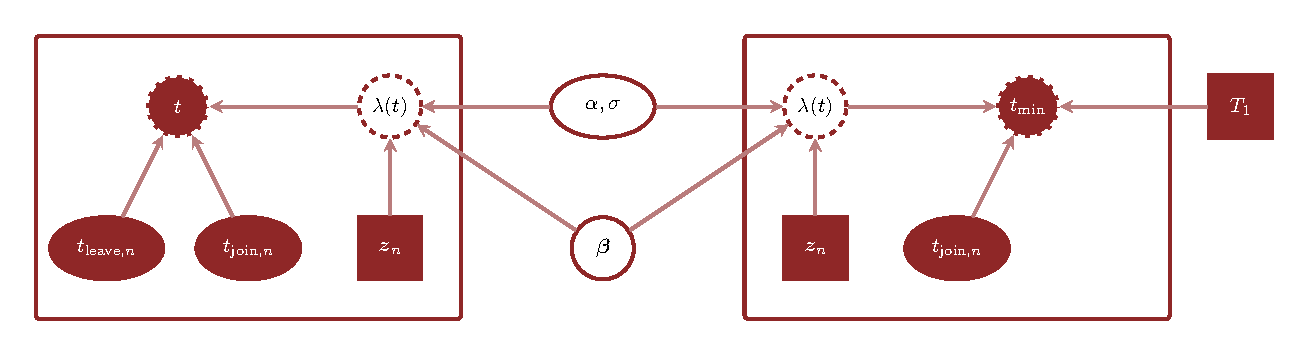
\includegraphics[width=1\textwidth,height=\textheight]{figures/dgms/model4/model4.pdf}

}

\caption{\label{fig-model4}A proportional stimulus survival model allows
the demographic variables to suppress or amplify the stimulus function,
which then modifies the behavior of the time-to-event model.}

\end{figure}%

Because the proportional scaling effectively modifies only the
\(\sigma\) parameter of the time-to-event model, we just need to compute
and then use \(\tau\) in place of \(\sigma\).

\begin{codelisting}

\caption{\texttt{model4.stan}}

\begin{Shaded}
\begin{Highlighting}[]
\KeywordTok{functions}\NormalTok{ \{}
  \CommentTok{// Log stimulus function}
  \DataTypeTok{real}\NormalTok{ log\_lambda(}\DataTypeTok{real}\NormalTok{ t, }\DataTypeTok{real}\NormalTok{ alpha, }\DataTypeTok{real}\NormalTok{ sigma) \{}
    \ControlFlowTok{return}\NormalTok{ log(alpha) {-} log(sigma) + (alpha {-} }\DecValTok{1}\NormalTok{) * log(t / sigma);}
\NormalTok{  \}}
  
  \CommentTok{// Cumulative stimulus function}
  \DataTypeTok{real}\NormalTok{ Lambda(}\DataTypeTok{real}\NormalTok{ t, }\DataTypeTok{real}\NormalTok{ alpha, }\DataTypeTok{real}\NormalTok{ sigma) \{}
    \ControlFlowTok{return}\NormalTok{ pow(t / sigma, alpha);}
\NormalTok{  \}}

  \CommentTok{// Log survival function}
  \DataTypeTok{real}\NormalTok{ log\_survival(}\DataTypeTok{real}\NormalTok{ t, }\DataTypeTok{real}\NormalTok{ alpha, }\DataTypeTok{real}\NormalTok{ sigma) \{}
    \ControlFlowTok{return}\NormalTok{ {-}Lambda(t, alpha, sigma);}
\NormalTok{  \}}

  \CommentTok{// Inverse cumulative stimulus function}
  \DataTypeTok{real}\NormalTok{ Lambda\_inv(}\DataTypeTok{real}\NormalTok{ l, }\DataTypeTok{real}\NormalTok{ alpha, }\DataTypeTok{real}\NormalTok{ sigma) \{}
    \ControlFlowTok{return}\NormalTok{ sigma * pow(l, }\DecValTok{1}\NormalTok{ / alpha);}
\NormalTok{  \}}
  
  \CommentTok{// Inverse survival function}
  \DataTypeTok{real}\NormalTok{ inv\_survival(}\DataTypeTok{real}\NormalTok{ u, }\DataTypeTok{real}\NormalTok{ alpha, }\DataTypeTok{real}\NormalTok{ sigma) \{}
    \ControlFlowTok{return}\NormalTok{ Lambda\_inv({-}log(u), alpha, sigma);}
\NormalTok{  \}}
\NormalTok{\}}

\KeywordTok{data}\NormalTok{ \{}
  \DataTypeTok{real}\NormalTok{           T0; }\CommentTok{// Months}
  \DataTypeTok{real}\NormalTok{\textless{}}\KeywordTok{lower}\NormalTok{=T0\textgreater{} T1; }\CommentTok{// Months}

  \DataTypeTok{int}\NormalTok{ I;            }\CommentTok{// Number of covariates}
  \DataTypeTok{row\_vector}\NormalTok{[I] z0; }\CommentTok{// Covariate baselines}

  \CommentTok{// Churned customers}
  \DataTypeTok{int}\NormalTok{\textless{}}\KeywordTok{lower}\NormalTok{=}\DecValTok{0}\NormalTok{\textgreater{} N\_churn;}
  \DataTypeTok{array}\NormalTok{[N\_churn] }\DataTypeTok{real}\NormalTok{\textless{}}\KeywordTok{lower}\NormalTok{=T0, }\KeywordTok{upper}\NormalTok{=T1\textgreater{} t\_join\_churn;  }\CommentTok{// Months}
  \DataTypeTok{array}\NormalTok{[N\_churn] }\DataTypeTok{real}\NormalTok{\textless{}}\KeywordTok{lower}\NormalTok{=T0, }\KeywordTok{upper}\NormalTok{=T1\textgreater{} t\_leave\_churn; }\CommentTok{// Months}

  \DataTypeTok{matrix}\NormalTok{[N\_churn, I] Z\_churn;}
  \DataTypeTok{array}\NormalTok{[N\_churn] }\DataTypeTok{int}\NormalTok{ online\_banking\_churn;}

  \CommentTok{// Active customers}
  \DataTypeTok{int}\NormalTok{\textless{}}\KeywordTok{lower}\NormalTok{=}\DecValTok{0}\NormalTok{\textgreater{} N\_active;}
  \DataTypeTok{array}\NormalTok{[N\_active] }\DataTypeTok{real}\NormalTok{\textless{}}\KeywordTok{lower}\NormalTok{=T0, }\KeywordTok{upper}\NormalTok{=T1\textgreater{} t\_join\_active; }\CommentTok{// Months}

  \DataTypeTok{matrix}\NormalTok{[N\_active, I] Z\_active;}
  \DataTypeTok{array}\NormalTok{[N\_active] }\DataTypeTok{int}\NormalTok{ online\_banking\_active;}
\NormalTok{\}}

\KeywordTok{parameters}\NormalTok{ \{}
  \DataTypeTok{real}\NormalTok{\textless{}}\KeywordTok{lower}\NormalTok{=}\DecValTok{0}\NormalTok{\textgreater{} omega; }\CommentTok{// Inverse shape parameter (Unitless)}
  \DataTypeTok{real}\NormalTok{\textless{}}\KeywordTok{lower}\NormalTok{=}\DecValTok{0}\NormalTok{\textgreater{} sigma; }\CommentTok{// Scale parameter (Months)}

  \DataTypeTok{vector}\NormalTok{[I] beta;    }\CommentTok{// Covariate slopes (1 / covariate units)}
  \DataTypeTok{real}\NormalTok{ delta\_online; }\CommentTok{// Online banking contribution}
\NormalTok{\}}

\KeywordTok{transformed parameters}\NormalTok{ \{}
  \DataTypeTok{real}\NormalTok{\textless{}}\KeywordTok{lower}\NormalTok{=}\DecValTok{0}\NormalTok{\textgreater{} alpha = }\DecValTok{1}\NormalTok{ / omega;}
\NormalTok{\}}

\KeywordTok{model}\NormalTok{ \{}
  \CommentTok{// Prior Model}
  \CommentTok{// 0 \textless{}\textasciitilde{} omega \textless{}\textasciitilde{} 1}
  \KeywordTok{target +=}\NormalTok{ normal\_lpdf(omega | }\DecValTok{0}\NormalTok{, }\DecValTok{1}\NormalTok{ / }\FloatTok{2.57}\NormalTok{);}

  \CommentTok{// 0 \textless{}\textasciitilde{} sigma \textless{}\textasciitilde{} 75}
  \KeywordTok{target +=}\NormalTok{ normal\_lpdf(sigma | }\DecValTok{0}\NormalTok{, }\DecValTok{75}\NormalTok{ / }\FloatTok{2.57}\NormalTok{);}

  \CommentTok{// {-}log(5) / 10 \textless{}\textasciitilde{} beta[1] \textless{}\textasciitilde{} +log(5) / 10}
  \KeywordTok{target +=}\NormalTok{ normal\_lpdf(beta[}\DecValTok{1}\NormalTok{] | }\DecValTok{0}\NormalTok{, }\FloatTok{0.07}\NormalTok{);}

  \CommentTok{// {-}log(5) / 1 \textless{}\textasciitilde{} beta[2] \textless{}\textasciitilde{} +log(5) / 1}
  \KeywordTok{target +=}\NormalTok{ normal\_lpdf(beta[}\DecValTok{2}\NormalTok{] | }\DecValTok{0}\NormalTok{, }\FloatTok{0.70}\NormalTok{);}

  \CommentTok{// {-}log(5) / 2 \textless{}\textasciitilde{} beta[3] \textless{}\textasciitilde{} +log(5) / 2}
  \KeywordTok{target +=}\NormalTok{ normal\_lpdf(beta[}\DecValTok{3}\NormalTok{] | }\DecValTok{0}\NormalTok{, }\FloatTok{0.35}\NormalTok{);}

  \CommentTok{// {-}log(5) / log(2) \textless{}\textasciitilde{} beta[4] \textless{}\textasciitilde{} +log(5) / log(2)}
  \KeywordTok{target +=}\NormalTok{ normal\_lpdf(beta[}\DecValTok{4}\NormalTok{] | }\DecValTok{0}\NormalTok{, }\DecValTok{1}\NormalTok{);}

  \CommentTok{// 0.1 \textless{}\textasciitilde{} exp(delta\_online) \textless{}\textasciitilde{} 10}
  \KeywordTok{target +=}\NormalTok{ normal\_lpdf(delta\_online | }\DecValTok{0}\NormalTok{, }\DecValTok{1}\NormalTok{);}

  \CommentTok{// Observational Model}
  \ControlFlowTok{for}\NormalTok{ (n }\ControlFlowTok{in} \DecValTok{1}\NormalTok{:N\_churn) \{}
    \DataTypeTok{real}\NormalTok{ tenure = t\_leave\_churn[n] {-} t\_join\_churn[n];}

    \DataTypeTok{real}\NormalTok{ mu = (Z\_churn[n,] {-} z0) * beta;}
    \ControlFlowTok{if}\NormalTok{ (online\_banking\_churn[n])}
\NormalTok{      mu += delta\_online;}
    \DataTypeTok{real}\NormalTok{ tau = sigma * exp({-}mu / alpha);}

    \KeywordTok{target +=}\NormalTok{   log\_lambda(tenure, alpha, tau)}
\NormalTok{              + log\_survival(tenure, alpha, tau);}
\NormalTok{  \}}

  \ControlFlowTok{for}\NormalTok{ (n }\ControlFlowTok{in} \DecValTok{1}\NormalTok{:N\_active) \{}
    \DataTypeTok{real}\NormalTok{ mu = (Z\_active[n,] {-} z0) * beta;}
    \ControlFlowTok{if}\NormalTok{ (online\_banking\_active[n])}
\NormalTok{      mu += delta\_online;}
    \DataTypeTok{real}\NormalTok{ tau = sigma * exp({-}mu / alpha);}

    \KeywordTok{target +=}\NormalTok{ log\_survival(T1 {-} t\_join\_active[n], alpha, tau);}
\NormalTok{  \}}
\NormalTok{\}}

\KeywordTok{generated quantities}\NormalTok{ \{}
  \DataTypeTok{array}\NormalTok{[N\_churn] }\DataTypeTok{real}\NormalTok{\textless{}}\KeywordTok{lower}\NormalTok{=}\DecValTok{0}\NormalTok{\textgreater{} tenure\_churn\_pred;}
  \DataTypeTok{array}\NormalTok{[N\_churn] }\DataTypeTok{real}\NormalTok{\textless{}}\KeywordTok{lower}\NormalTok{=T0\textgreater{} t\_leave\_churn\_pred;}

  \ControlFlowTok{for}\NormalTok{ (n }\ControlFlowTok{in} \DecValTok{1}\NormalTok{:N\_churn) \{}
    \DataTypeTok{real}\NormalTok{ mu = (Z\_churn[n,] {-} z0) * beta;}
    \ControlFlowTok{if}\NormalTok{ (online\_banking\_churn[n])}
\NormalTok{      mu += delta\_online;}
    \DataTypeTok{real}\NormalTok{ tau = sigma * exp({-}mu / alpha);}

    \DataTypeTok{real}\NormalTok{ S = exp(log\_survival(T1 {-} t\_join\_churn[n],}
\NormalTok{                              alpha, tau));}
    \DataTypeTok{real}\NormalTok{ u = uniform\_rng(S, }\DecValTok{1}\NormalTok{);}
\NormalTok{    tenure\_churn\_pred[n]}
\NormalTok{      = inv\_survival(u, alpha, tau);}
\NormalTok{    t\_leave\_churn\_pred[n]}
\NormalTok{      = t\_join\_churn[n] + tenure\_churn\_pred[n];}
\NormalTok{  \}}
\NormalTok{\}}
\end{Highlighting}
\end{Shaded}

\end{codelisting}

\begin{Shaded}
\begin{Highlighting}[]
\ControlFlowTok{with} \BuiltInTok{open}\NormalTok{(}\StringTok{\textquotesingle{}stan\_programs/model4.stan\textquotesingle{}}\NormalTok{, }\StringTok{\textquotesingle{}r\textquotesingle{}}\NormalTok{) }\ImportTok{as} \BuiltInTok{file}\NormalTok{:}
\NormalTok{  stan\_program }\OperatorTok{=} \BuiltInTok{file}\NormalTok{.read()}
\NormalTok{model }\OperatorTok{=}\NormalTok{ stan.build(stan\_program,}
\NormalTok{                   random\_seed}\OperatorTok{=}\DecValTok{8438338}\NormalTok{,}
\NormalTok{                   data}\OperatorTok{=}\NormalTok{stan\_data)}
\NormalTok{fit }\OperatorTok{=}\NormalTok{ model.sample(num\_samples}\OperatorTok{=}\DecValTok{1024}\NormalTok{, refresh}\OperatorTok{=}\DecValTok{0}\NormalTok{)}
\end{Highlighting}
\end{Shaded}

\begin{verbatim}
Building...
\end{verbatim}

Hamiltonian Monte Carlo remains undaunted by our increasingly-complex
posterior distributions.

\begin{Shaded}
\begin{Highlighting}[]
\NormalTok{diagnostics }\OperatorTok{=}\NormalTok{ util.extract\_hmc\_diagnostics(fit)}
\NormalTok{util.check\_all\_hmc\_diagnostics(diagnostics)}

\NormalTok{samples }\OperatorTok{=}\NormalTok{ util.extract\_expectand\_vals(fit)}
\NormalTok{base\_samples }\OperatorTok{=}\NormalTok{ util.filter\_expectands(samples,}
\NormalTok{                                      [}\StringTok{\textquotesingle{}omega\textquotesingle{}}\NormalTok{, }\StringTok{\textquotesingle{}sigma\textquotesingle{}}\NormalTok{,}
                                       \StringTok{\textquotesingle{}beta\textquotesingle{}}\NormalTok{, }\StringTok{\textquotesingle{}delta\_online\textquotesingle{}}\NormalTok{],}
\NormalTok{                                      check\_arrays}\OperatorTok{=}\VariableTok{True}\NormalTok{)}
\NormalTok{util.check\_all\_expectand\_diagnostics(base\_samples)}
\end{Highlighting}
\end{Shaded}

\begin{verbatim}
All Hamiltonian Monte Carlo diagnostics are consistent with accurate
Markov chain Monte Carlo.
 
All expectands checked appear to be behaving well enough for reliable
Markov chain Monte Carlo estimation.
 
\end{verbatim}

\subsection{Posterior Retrodictive
Checks}\label{posterior-retrodictive-checks-3}

After all of this modeling work, the payoff is pretty rewarding. By
incorporating demographic heterogeneity, our new model exhibits
beautiful retrodictive agreement across all of the summaries that we
have considered so far.

\begin{Shaded}
\begin{Highlighting}[]
\NormalTok{f, axarr }\OperatorTok{=}\NormalTok{ plot.subplots(}\DecValTok{2}\NormalTok{, }\DecValTok{1}\NormalTok{, layout}\OperatorTok{=}\StringTok{"constrained"}\NormalTok{)}

\NormalTok{putil.plot\_hist\_quantiles(}
\NormalTok{  axarr[}\DecValTok{0}\NormalTok{], samples, }\StringTok{\textquotesingle{}tenure\_churn\_pred\textquotesingle{}}\NormalTok{,}
\NormalTok{  data[}\StringTok{\textquotesingle{}T0\textquotesingle{}}\NormalTok{] }\OperatorTok{{-}} \DecValTok{1}\NormalTok{, data[}\StringTok{\textquotesingle{}T1\textquotesingle{}}\NormalTok{] }\OperatorTok{+} \DecValTok{1}\NormalTok{, }\DecValTok{1}\NormalTok{,}
\NormalTok{  baseline\_values}\OperatorTok{=}\NormalTok{tenure\_churn,}
\NormalTok{  xlabel}\OperatorTok{=}\StringTok{\textquotesingle{}Customer Tenure (months)\textquotesingle{}}
\NormalTok{)}


\NormalTok{putil.plot\_hist\_quantiles(}
\NormalTok{  axarr[}\DecValTok{1}\NormalTok{], samples, }\StringTok{\textquotesingle{}t\_leave\_churn\_pred\textquotesingle{}}\NormalTok{,}
\NormalTok{  data[}\StringTok{\textquotesingle{}T0\textquotesingle{}}\NormalTok{] }\OperatorTok{{-}} \DecValTok{3}\NormalTok{, data[}\StringTok{\textquotesingle{}T1\textquotesingle{}}\NormalTok{] }\OperatorTok{+} \DecValTok{23}\NormalTok{, }\DecValTok{3}\NormalTok{,}
\NormalTok{  baseline\_values}\OperatorTok{=}\NormalTok{data[}\StringTok{\textquotesingle{}t\_leave\_churn\textquotesingle{}}\NormalTok{],}
\NormalTok{  xlabel}\OperatorTok{=}\StringTok{"Time Customer Leaves (months)"}
\NormalTok{)}
\NormalTok{axarr[}\DecValTok{1}\NormalTok{].axvline(x}\OperatorTok{=}\NormalTok{data[}\StringTok{\textquotesingle{}T0\textquotesingle{}}\NormalTok{], linewidth}\OperatorTok{=}\DecValTok{2}\NormalTok{,}
\NormalTok{                 linestyle}\OperatorTok{=}\StringTok{\textquotesingle{}dashed\textquotesingle{}}\NormalTok{, color}\OperatorTok{=}\StringTok{"\#DDDDDD"}\NormalTok{)}
\NormalTok{axarr[}\DecValTok{1}\NormalTok{].axvline(x}\OperatorTok{=}\NormalTok{data[}\StringTok{\textquotesingle{}T1\textquotesingle{}}\NormalTok{], linewidth}\OperatorTok{=}\DecValTok{2}\NormalTok{,}
\NormalTok{                 linestyle}\OperatorTok{=}\StringTok{\textquotesingle{}dashed\textquotesingle{}}\NormalTok{, color}\OperatorTok{=}\StringTok{"\#DDDDDD"}\NormalTok{)}

\NormalTok{plot.show()}
\end{Highlighting}
\end{Shaded}

\includegraphics{churn_files/figure-pdf/cell-52-output-1.png}

In particular, there's no indication that our demographic proportion
model is inadequate, at least for the observed customer demographics.

\begin{Shaded}
\begin{Highlighting}[]
\NormalTok{pred\_names }\OperatorTok{=}\NormalTok{ [ }\SpecialStringTok{f\textquotesingle{}tenure\_churn\_pred[}\SpecialCharTok{\{}\NormalTok{n }\OperatorTok{+} \DecValTok{1}\SpecialCharTok{\}}\SpecialStringTok{]\textquotesingle{}}
               \ControlFlowTok{for}\NormalTok{ n }\KeywordTok{in} \BuiltInTok{range}\NormalTok{(data[}\StringTok{\textquotesingle{}N\_churn\textquotesingle{}}\NormalTok{]) ]}

\NormalTok{f, axarr }\OperatorTok{=}\NormalTok{ plot.subplots(}\DecValTok{2}\NormalTok{, }\DecValTok{2}\NormalTok{, layout}\OperatorTok{=}\StringTok{"constrained"}\NormalTok{)}

\ControlFlowTok{for}\NormalTok{ i }\KeywordTok{in} \BuiltInTok{range}\NormalTok{(data[}\StringTok{\textquotesingle{}I\textquotesingle{}}\NormalTok{]):}
\NormalTok{  i1 }\OperatorTok{=}\NormalTok{ i }\OperatorTok{//} \DecValTok{2}
\NormalTok{  i2 }\OperatorTok{=}\NormalTok{ i }\OperatorTok{\%} \DecValTok{2}

\NormalTok{  putil.plot\_conditional\_median\_quantiles(}
\NormalTok{    axarr[i1, i2], samples, pred\_names,}
\NormalTok{    [ z[i] }\ControlFlowTok{for}\NormalTok{ z }\KeywordTok{in}\NormalTok{ Z\_churn ],}
\NormalTok{    bin\_min[i], bin\_max[i], bin\_delta[i],}
\NormalTok{    tenure\_churn, residual}\OperatorTok{=}\VariableTok{False}\NormalTok{,}
\NormalTok{    xlabel}\OperatorTok{=}\NormalTok{z\_names[i], ylabel}\OperatorTok{=}\StringTok{""}
\NormalTok{  )}

\NormalTok{plot.show()}
\end{Highlighting}
\end{Shaded}

\begin{verbatim}
1 conditioning values (0.04%) fell below the histogram binning.
18 conditioning values (0.80%) fell above the histogram binning.
\end{verbatim}

\includegraphics{churn_files/figure-pdf/cell-53-output-2.png}

Failures of the exponential-linear proportion model would manifest as
disagreement in these conditional median plots. Moreover, the shape of
the residual difference between the posterior predictive and observed
behaviors would directly inform the inadequacies of our initial
functional model, and hence how to improve it.

\subsection{Posterior Inferences}\label{posterior-inferences}

Now that none of our posterior retrodictive checks suggest any model
inadequacies, we can interpret the derived posterior inferences as
reasonable approximations to the true data generating behavior.

\begin{Shaded}
\begin{Highlighting}[]
\NormalTok{f, axarr }\OperatorTok{=}\NormalTok{ plot.subplots(}\DecValTok{1}\NormalTok{, }\DecValTok{3}\NormalTok{, layout}\OperatorTok{=}\StringTok{"constrained"}\NormalTok{)}

\NormalTok{util.plot\_expectand\_pushforward(axarr[}\DecValTok{0}\NormalTok{], samples[}\StringTok{\textquotesingle{}alpha\textquotesingle{}}\NormalTok{],}
                                \DecValTok{25}\NormalTok{, flim}\OperatorTok{=}\NormalTok{[}\FloatTok{1.3}\NormalTok{, }\FloatTok{1.6}\NormalTok{],}
\NormalTok{                                display\_name}\OperatorTok{=}\StringTok{"alpha"}\NormalTok{)}

\NormalTok{util.plot\_expectand\_pushforward(axarr[}\DecValTok{1}\NormalTok{], samples[}\StringTok{\textquotesingle{}sigma\textquotesingle{}}\NormalTok{],}
                                \DecValTok{25}\NormalTok{, flim}\OperatorTok{=}\NormalTok{[}\FloatTok{3.75}\NormalTok{, }\FloatTok{5.25}\NormalTok{],}
\NormalTok{                                display\_name}\OperatorTok{=}\StringTok{"sigma"}\NormalTok{)}

\NormalTok{util.plot\_expectand\_pushforward(axarr[}\DecValTok{2}\NormalTok{], samples[}\StringTok{\textquotesingle{}delta\_online\textquotesingle{}}\NormalTok{],}
                                \DecValTok{25}\NormalTok{, flim}\OperatorTok{=}\NormalTok{[}\OperatorTok{{-}}\FloatTok{0.25}\NormalTok{, }\FloatTok{0.25}\NormalTok{],}
\NormalTok{                                display\_name}\OperatorTok{=}\StringTok{"delta\_online"}\NormalTok{)}
\NormalTok{plot.show()}
\end{Highlighting}
\end{Shaded}

\includegraphics{churn_files/figure-pdf/cell-54-output-1.png}

We can see, for example, that the stimulus function, and the speed at
which customers leave, deceases when any of the demographic variables
move above their baseline values. Moreover, the decrease is most
sensitive to increases in the logit wealth percentile.

\begin{Shaded}
\begin{Highlighting}[]
\NormalTok{names }\OperatorTok{=}\NormalTok{ [ }\SpecialStringTok{f\textquotesingle{}beta[}\SpecialCharTok{\{}\NormalTok{i }\OperatorTok{+} \DecValTok{1}\SpecialCharTok{\}}\SpecialStringTok{]\textquotesingle{}}
          \ControlFlowTok{for}\NormalTok{ i }\KeywordTok{in} \BuiltInTok{range}\NormalTok{(data[}\StringTok{\textquotesingle{}I\textquotesingle{}}\NormalTok{]) ]}
\NormalTok{putil.plot\_disc\_pushforward\_quantiles\_vert(}
\NormalTok{  plot.gca(), samples, names,}
\NormalTok{  yticklabels}\OperatorTok{=}\NormalTok{names,}
\NormalTok{  xlabel}\OperatorTok{=}\StringTok{"Marginal Posterior Quantiles"}
\NormalTok{)}

\NormalTok{plot.show()}
\end{Highlighting}
\end{Shaded}

\includegraphics{churn_files/figure-pdf/cell-55-output-1.png}

\section{Customer Lifetime Value By
Segment}\label{customer-lifetime-value-by-segment}

Now the real fun begins. Our posterior inferences can be used to not
only learn about the customers observed in our study, but also make
predictions for the behavior of new, unobserved customers.

For example, let's say that the bank's potential customer base has been
stratified into segments, each of which is characterized by an ensemble
of representative demographic configurations.

\begin{Shaded}
\begin{Highlighting}[]
\ControlFlowTok{with} \BuiltInTok{open}\NormalTok{(}\StringTok{"data/customer\_segmentation.json"}\NormalTok{, }\StringTok{"r"}\NormalTok{) }\ImportTok{as}\NormalTok{ infile:}
\NormalTok{  customer\_segmentation }\OperatorTok{=}\NormalTok{ json.load(infile)}
\end{Highlighting}
\end{Shaded}

\begin{Shaded}
\begin{Highlighting}[]
\ControlFlowTok{for}\NormalTok{ i, name }\KeywordTok{in} \BuiltInTok{enumerate}\NormalTok{(customer\_segmentation[}\StringTok{\textquotesingle{}segment\_names\textquotesingle{}}\NormalTok{]):}
  \BuiltInTok{print}\NormalTok{(}\SpecialStringTok{f\textquotesingle{}Segment }\SpecialCharTok{\{}\NormalTok{i }\OperatorTok{+} \DecValTok{1}\SpecialCharTok{\}}\SpecialStringTok{: }\SpecialCharTok{\{}\NormalTok{name}\SpecialCharTok{\}}\SpecialStringTok{\textquotesingle{}}\NormalTok{)}
\end{Highlighting}
\end{Shaded}

\begin{verbatim}
Segment 1: Mass Retail
Segment 2: Private Banking
Segment 3: Wealth
Segment 4: Retired
Segment 5: Young Professional
Segment 6: Student
\end{verbatim}

The customers in the private banking segment are older and more wealthy
than the customers in the student segment.

\begin{Shaded}
\begin{Highlighting}[]
\NormalTok{bin\_min }\OperatorTok{=}\NormalTok{ [ }\DecValTok{0}\NormalTok{, }\DecValTok{0}\NormalTok{, }\DecValTok{0}\NormalTok{, }\DecValTok{0}\NormalTok{ ]}
\NormalTok{bin\_max }\OperatorTok{=}\NormalTok{ [ }\DecValTok{100}\NormalTok{, }\DecValTok{15}\NormalTok{, }\FloatTok{1.05}\NormalTok{, }\DecValTok{1000}\NormalTok{ ]}
\NormalTok{bin\_delta }\OperatorTok{=}\NormalTok{ [ }\DecValTok{5}\NormalTok{, }\DecValTok{1}\NormalTok{, }\FloatTok{0.05}\NormalTok{, }\DecValTok{10}\NormalTok{ ]}

\NormalTok{f, axarr }\OperatorTok{=}\NormalTok{ plot.subplots(}\DecValTok{2}\NormalTok{, }\DecValTok{2}\NormalTok{, layout}\OperatorTok{=}\StringTok{"constrained"}\NormalTok{)}

\ControlFlowTok{for}\NormalTok{ i }\KeywordTok{in} \BuiltInTok{range}\NormalTok{(data[}\StringTok{\textquotesingle{}I\textquotesingle{}}\NormalTok{]):}
\NormalTok{  i1 }\OperatorTok{=}\NormalTok{ i }\OperatorTok{//} \DecValTok{2}
\NormalTok{  i2 }\OperatorTok{=}\NormalTok{ i }\OperatorTok{\%} \DecValTok{2}

\NormalTok{  putil.plot\_line\_hists(axarr[i1, i2],}
\NormalTok{                        [ x[i] }\ControlFlowTok{for}\NormalTok{ s, x }\KeywordTok{in}
                          \BuiltInTok{zip}\NormalTok{(customer\_segmentation[}\StringTok{\textquotesingle{}customer\_segment\_pred\textquotesingle{}}\NormalTok{],}
\NormalTok{                              customer\_segmentation[}\StringTok{\textquotesingle{}X\_pred\textquotesingle{}}\NormalTok{])}
                          \ControlFlowTok{if}\NormalTok{ s }\OperatorTok{==} \DecValTok{1}\NormalTok{ ],}
\NormalTok{                        [ x[i] }\ControlFlowTok{for}\NormalTok{ s, x }\KeywordTok{in}
                          \BuiltInTok{zip}\NormalTok{(customer\_segmentation[}\StringTok{\textquotesingle{}customer\_segment\_pred\textquotesingle{}}\NormalTok{],}
\NormalTok{                              customer\_segmentation[}\StringTok{\textquotesingle{}X\_pred\textquotesingle{}}\NormalTok{])}
                          \ControlFlowTok{if}\NormalTok{ s }\OperatorTok{==} \DecValTok{5}\NormalTok{ ],}
\NormalTok{                       bin\_min[i], bin\_max[i], bin\_delta[i],}
\NormalTok{                       xlabel}\OperatorTok{=}\NormalTok{data[}\StringTok{\textquotesingle{}x\_names\textquotesingle{}}\NormalTok{][i])}

\NormalTok{plot.show()}
\end{Highlighting}
\end{Shaded}

\includegraphics{churn_files/figure-pdf/cell-58-output-1.png}

When can use our model to predict how loyal the customers in each of
these segments might be, and hence what their lifetime value to the bank
might be. To be meticulous, we have to account for future discounting
over the lifetime of a customer.

\begin{Shaded}
\begin{Highlighting}[]
\NormalTok{stan\_data[}\StringTok{\textquotesingle{}S\textquotesingle{}}\NormalTok{] }\OperatorTok{=}\NormalTok{ customer\_segmentation[}\StringTok{\textquotesingle{}S\textquotesingle{}}\NormalTok{]}

\NormalTok{stan\_data[}\StringTok{\textquotesingle{}segment\_pred\textquotesingle{}}\NormalTok{] }\OperatorTok{=} \OperatorTok{\textbackslash{}}
\NormalTok{  customer\_segmentation[}\StringTok{\textquotesingle{}customer\_segment\_pred\textquotesingle{}}\NormalTok{]}
\end{Highlighting}
\end{Shaded}

\begin{Shaded}
\begin{Highlighting}[]
\NormalTok{stan\_data[}\StringTok{\textquotesingle{}value\_per\_month\textquotesingle{}}\NormalTok{] }\OperatorTok{=}\NormalTok{ [}
  \DecValTok{50}\NormalTok{,  }\CommentTok{\# Mass Retail}
  \DecValTok{75}\NormalTok{, }\CommentTok{\# Private Banking}
  \DecValTok{80}\NormalTok{, }\CommentTok{\# Wealth}
  \DecValTok{45}\NormalTok{, }\CommentTok{\# Retired}
  \DecValTok{60}\NormalTok{,  }\CommentTok{\# Young Professional}
  \DecValTok{40}\NormalTok{,  }\CommentTok{\# Student}
\NormalTok{]}

\NormalTok{stan\_data[}\StringTok{\textquotesingle{}zero\_rate\textquotesingle{}}\NormalTok{] }\OperatorTok{=} \FloatTok{0.10}
\end{Highlighting}
\end{Shaded}

If we also know how expensive customers in each of these segments are to
acquire, then we can use these inferences to identify the most most
profitable type of customers.

\begin{Shaded}
\begin{Highlighting}[]
\NormalTok{stan\_data[}\StringTok{\textquotesingle{}acq\_cost\textquotesingle{}}\NormalTok{] }\OperatorTok{=}\NormalTok{ [}
  \DecValTok{150}\NormalTok{,  }\CommentTok{\# Mass Retail}
  \DecValTok{310}\NormalTok{, }\CommentTok{\# Private Banking}
  \DecValTok{260}\NormalTok{, }\CommentTok{\# Wealth}
  \DecValTok{175}\NormalTok{, }\CommentTok{\# Retired}
  \DecValTok{175}\NormalTok{,  }\CommentTok{\# Young Professional}
  \DecValTok{125}\NormalTok{,  }\CommentTok{\# Student}
\NormalTok{]}
\end{Highlighting}
\end{Shaded}

\subsection{Posterior Quantification}\label{posterior-quantification-4}

Because our inferences are the same, the basic structure of the full
Bayesian model is the same. We just have to add the derived predictions
(Figure~\ref{fig-model5}).

\begin{figure}

\centering{

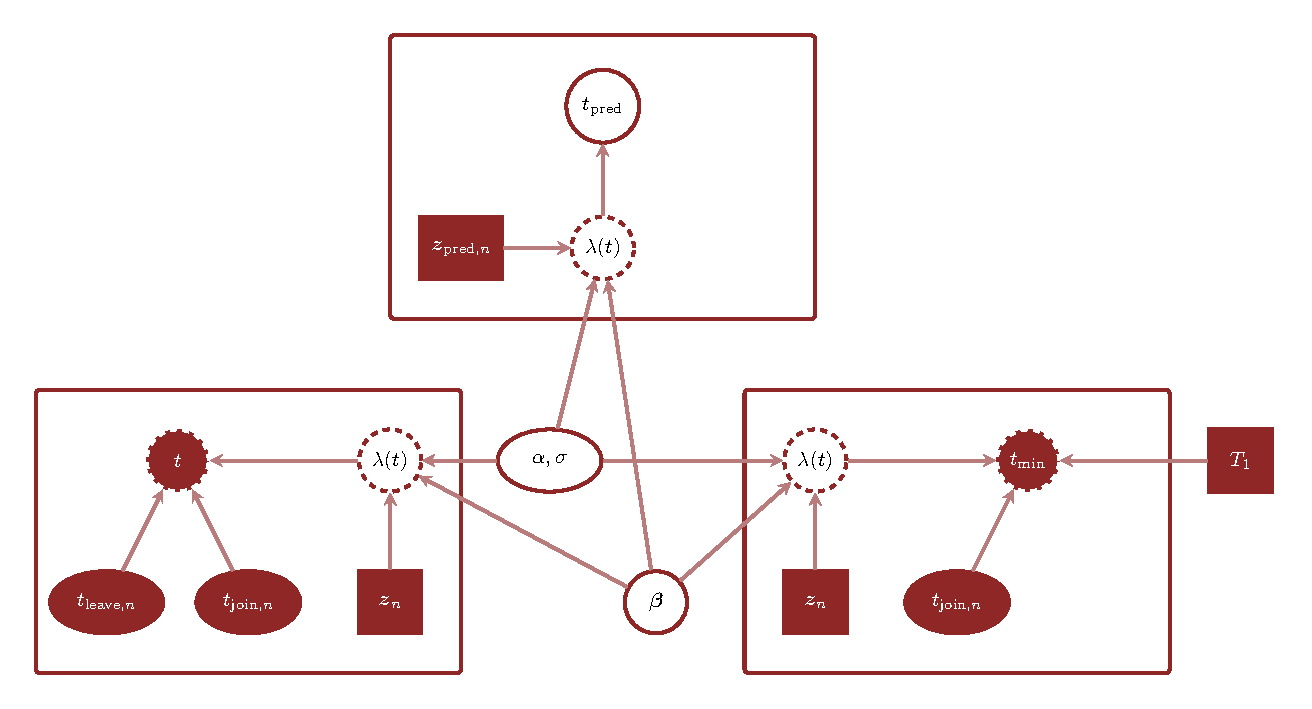
\includegraphics[width=1\textwidth,height=\textheight]{figures/dgms/model5/model5.pdf}

}

\caption{\label{fig-model5}Once we've learned the consistent
configurations of our model, we can make predictions for new customers.}

\end{figure}%

In our Stan program, we need to pass in the segment demographics and
then calculate predictions in the \texttt{generated\ quantities} block.

\begin{codelisting}

\caption{\texttt{model5.stan}}

\begin{Shaded}
\begin{Highlighting}[]
\KeywordTok{functions}\NormalTok{ \{}
  \CommentTok{// Log stimulus function}
  \DataTypeTok{real}\NormalTok{ log\_lambda(}\DataTypeTok{real}\NormalTok{ t, }\DataTypeTok{real}\NormalTok{ alpha, }\DataTypeTok{real}\NormalTok{ sigma) \{}
    \ControlFlowTok{return}\NormalTok{ log(alpha) {-} log(sigma) + (alpha {-} }\DecValTok{1}\NormalTok{) * log(t / sigma);}
\NormalTok{  \}}
  
  \CommentTok{// Cumulative stimulus function}
  \DataTypeTok{real}\NormalTok{ Lambda(}\DataTypeTok{real}\NormalTok{ t, }\DataTypeTok{real}\NormalTok{ alpha, }\DataTypeTok{real}\NormalTok{ sigma) \{}
    \ControlFlowTok{return}\NormalTok{ pow(t / sigma, alpha);}
\NormalTok{  \}}

  \CommentTok{// Log survival function}
  \DataTypeTok{real}\NormalTok{ log\_survival(}\DataTypeTok{real}\NormalTok{ t, }\DataTypeTok{real}\NormalTok{ alpha, }\DataTypeTok{real}\NormalTok{ sigma) \{}
    \ControlFlowTok{return}\NormalTok{ {-}Lambda(t, alpha, sigma);}
\NormalTok{  \}}

  \CommentTok{// Inverse cumulative stimulus function}
  \DataTypeTok{real}\NormalTok{ Lambda\_inv(}\DataTypeTok{real}\NormalTok{ l, }\DataTypeTok{real}\NormalTok{ alpha, }\DataTypeTok{real}\NormalTok{ sigma) \{}
    \ControlFlowTok{return}\NormalTok{ sigma * pow(l, }\DecValTok{1}\NormalTok{ / alpha);}
\NormalTok{  \}}
  
  \CommentTok{// Inverse survival function}
  \DataTypeTok{real}\NormalTok{ inv\_survival(}\DataTypeTok{real}\NormalTok{ u, }\DataTypeTok{real}\NormalTok{ alpha, }\DataTypeTok{real}\NormalTok{ sigma) \{}
    \ControlFlowTok{return}\NormalTok{ Lambda\_inv({-}log(u), alpha, sigma);}
\NormalTok{  \}}
\NormalTok{\}}

\KeywordTok{data}\NormalTok{ \{}
  \DataTypeTok{real}\NormalTok{           T0; }\CommentTok{// Months}
  \DataTypeTok{real}\NormalTok{\textless{}}\KeywordTok{lower}\NormalTok{=T0\textgreater{} T1; }\CommentTok{// Months}

  \DataTypeTok{int}\NormalTok{ I;            }\CommentTok{// Number of covariates}
  \DataTypeTok{row\_vector}\NormalTok{[I] z0; }\CommentTok{// Covariate baselines}

  \CommentTok{// Churned customers}
  \DataTypeTok{int}\NormalTok{\textless{}}\KeywordTok{lower}\NormalTok{=}\DecValTok{0}\NormalTok{\textgreater{} N\_churn;}
  \DataTypeTok{array}\NormalTok{[N\_churn] }\DataTypeTok{real}\NormalTok{\textless{}}\KeywordTok{lower}\NormalTok{=T0, }\KeywordTok{upper}\NormalTok{=T1\textgreater{} t\_join\_churn;  }\CommentTok{// Months}
  \DataTypeTok{array}\NormalTok{[N\_churn] }\DataTypeTok{real}\NormalTok{\textless{}}\KeywordTok{lower}\NormalTok{=T0, }\KeywordTok{upper}\NormalTok{=T1\textgreater{} t\_leave\_churn; }\CommentTok{// Months}

  \DataTypeTok{matrix}\NormalTok{[N\_churn, I] Z\_churn;}
  \DataTypeTok{array}\NormalTok{[N\_churn] }\DataTypeTok{int}\NormalTok{ online\_banking\_churn;}

  \CommentTok{// Active customers}
  \DataTypeTok{int}\NormalTok{\textless{}}\KeywordTok{lower}\NormalTok{=}\DecValTok{0}\NormalTok{\textgreater{} N\_active;}
  \DataTypeTok{array}\NormalTok{[N\_active] }\DataTypeTok{real}\NormalTok{\textless{}}\KeywordTok{lower}\NormalTok{=T0, }\KeywordTok{upper}\NormalTok{=T1\textgreater{} t\_join\_active; }\CommentTok{// Months}

  \DataTypeTok{matrix}\NormalTok{[N\_active, I] Z\_active;}
  \DataTypeTok{array}\NormalTok{[N\_active] }\DataTypeTok{int}\NormalTok{ online\_banking\_active;}

  \CommentTok{// Prospective customers}
  \DataTypeTok{int}\NormalTok{\textless{}}\KeywordTok{lower}\NormalTok{=}\DecValTok{0}\NormalTok{\textgreater{} N\_pred;}

  \DataTypeTok{matrix}\NormalTok{[N\_pred, I] Z\_pred;}
  \DataTypeTok{array}\NormalTok{[N\_pred] }\DataTypeTok{int}\NormalTok{ online\_banking\_pred;}

  \DataTypeTok{int}\NormalTok{\textless{}}\KeywordTok{lower}\NormalTok{=}\DecValTok{0}\NormalTok{\textgreater{} S; }\CommentTok{// Number of segments}
  \DataTypeTok{array}\NormalTok{[N\_pred] }\DataTypeTok{int}\NormalTok{\textless{}}\KeywordTok{lower}\NormalTok{=}\DecValTok{1}\NormalTok{, }\KeywordTok{upper}\NormalTok{=S\textgreater{} segment\_pred;}

  \DataTypeTok{array}\NormalTok{[S] }\DataTypeTok{real}\NormalTok{\textless{}}\KeywordTok{lower}\NormalTok{=}\DecValTok{0}\NormalTok{\textgreater{} value\_per\_month; }\CommentTok{// Euros / Month}
  \DataTypeTok{real}\NormalTok{\textless{}}\KeywordTok{lower}\NormalTok{=}\DecValTok{0}\NormalTok{, }\KeywordTok{upper}\NormalTok{=}\DecValTok{1}\NormalTok{\textgreater{} zero\_rate; }\CommentTok{// Percentage / Year}

  \DataTypeTok{array}\NormalTok{[S] }\DataTypeTok{real}\NormalTok{\textless{}}\KeywordTok{lower}\NormalTok{=}\DecValTok{0}\NormalTok{\textgreater{} acq\_cost;  }\CommentTok{// Euros}
\NormalTok{\}}

\KeywordTok{parameters}\NormalTok{ \{}
  \DataTypeTok{real}\NormalTok{\textless{}}\KeywordTok{lower}\NormalTok{=}\DecValTok{0}\NormalTok{\textgreater{} omega; }\CommentTok{// Inverse shape parameter (Unitless)}
  \DataTypeTok{real}\NormalTok{\textless{}}\KeywordTok{lower}\NormalTok{=}\DecValTok{0}\NormalTok{\textgreater{} sigma; }\CommentTok{// Scale parameter (Months)}

  \DataTypeTok{vector}\NormalTok{[I] beta;    }\CommentTok{// Covariate slopes (1 / covariate units)}
  \DataTypeTok{real}\NormalTok{ delta\_online; }\CommentTok{// Online banking contribution}
\NormalTok{\}}

\KeywordTok{transformed parameters}\NormalTok{ \{}
  \DataTypeTok{real}\NormalTok{\textless{}}\KeywordTok{lower}\NormalTok{=}\DecValTok{0}\NormalTok{\textgreater{} alpha = }\DecValTok{1}\NormalTok{ / omega;}
\NormalTok{\}}

\KeywordTok{model}\NormalTok{ \{}
  \CommentTok{// Prior Model}
  \KeywordTok{target +=}\NormalTok{ normal\_lpdf(omega | }\DecValTok{0}\NormalTok{, }\DecValTok{1}\NormalTok{ / }\FloatTok{2.57}\NormalTok{);}
  \KeywordTok{target +=}\NormalTok{ normal\_lpdf(sigma | }\DecValTok{0}\NormalTok{, }\DecValTok{75}\NormalTok{ / }\FloatTok{2.57}\NormalTok{);}
  \KeywordTok{target +=}\NormalTok{ normal\_lpdf(beta[}\DecValTok{1}\NormalTok{] | }\DecValTok{0}\NormalTok{, }\FloatTok{0.07}\NormalTok{);}
  \KeywordTok{target +=}\NormalTok{ normal\_lpdf(beta[}\DecValTok{2}\NormalTok{] | }\DecValTok{0}\NormalTok{, }\FloatTok{0.70}\NormalTok{);}
  \KeywordTok{target +=}\NormalTok{ normal\_lpdf(beta[}\DecValTok{3}\NormalTok{] | }\DecValTok{0}\NormalTok{, }\FloatTok{0.35}\NormalTok{);}
  \KeywordTok{target +=}\NormalTok{ normal\_lpdf(beta[}\DecValTok{4}\NormalTok{] | }\DecValTok{0}\NormalTok{, }\DecValTok{1}\NormalTok{);}
  \KeywordTok{target +=}\NormalTok{ normal\_lpdf(delta\_online | }\DecValTok{0}\NormalTok{, }\DecValTok{1}\NormalTok{);}

  \CommentTok{// Observational Model}
  \ControlFlowTok{for}\NormalTok{ (n }\ControlFlowTok{in} \DecValTok{1}\NormalTok{:N\_churn) \{}
    \DataTypeTok{real}\NormalTok{ tenure = t\_leave\_churn[n] {-} t\_join\_churn[n];}

    \DataTypeTok{real}\NormalTok{ mu = (Z\_churn[n,] {-} z0) * beta;}
    \ControlFlowTok{if}\NormalTok{ (online\_banking\_churn[n])}
\NormalTok{      mu += delta\_online;}
    \DataTypeTok{real}\NormalTok{ tau = sigma * exp({-}mu / alpha);}

    \KeywordTok{target +=}\NormalTok{   log\_lambda(tenure, alpha, tau)}
\NormalTok{              + log\_survival(tenure, alpha, tau);}
\NormalTok{  \}}

  \ControlFlowTok{for}\NormalTok{ (n }\ControlFlowTok{in} \DecValTok{1}\NormalTok{:N\_active) \{}
    \DataTypeTok{real}\NormalTok{ mu = (Z\_active[n,] {-} z0) * beta;}
    \ControlFlowTok{if}\NormalTok{ (online\_banking\_active[n])}
\NormalTok{      mu += delta\_online;}
    \DataTypeTok{real}\NormalTok{ tau = sigma * exp({-}mu / alpha);}

    \KeywordTok{target +=}\NormalTok{ log\_survival(T1 {-} t\_join\_active[n], alpha, tau);}
\NormalTok{  \}}
\NormalTok{\}}

\KeywordTok{generated quantities}\NormalTok{ \{}
  \DataTypeTok{array}\NormalTok{[N\_pred] }\DataTypeTok{real}\NormalTok{\textless{}}\KeywordTok{lower}\NormalTok{=}\DecValTok{0}\NormalTok{\textgreater{} clv\_discount;}
  \DataTypeTok{array}\NormalTok{[N\_pred] }\DataTypeTok{real}\NormalTok{ profit;}

  \ControlFlowTok{for}\NormalTok{ (n }\ControlFlowTok{in} \DecValTok{1}\NormalTok{:N\_pred) \{}
    \DataTypeTok{real}\NormalTok{ mu = (Z\_pred[n,] {-} z0) * beta;}
    \ControlFlowTok{if}\NormalTok{ (online\_banking\_pred[n])}
\NormalTok{      mu += delta\_online;}
    \DataTypeTok{real}\NormalTok{ tau = sigma * exp({-}mu / alpha);}

    \DataTypeTok{real}\NormalTok{ u = uniform\_rng(}\DecValTok{0}\NormalTok{, }\DecValTok{1}\NormalTok{);}
    \DataTypeTok{real}\NormalTok{ tenure = inv\_survival(u, alpha, tau);}

    \DataTypeTok{int}\NormalTok{ s = segment\_pred[n];}

\NormalTok{    clv\_discount[n] = value\_per\_month[s] * tenure /}
\NormalTok{                      pow(}\DecValTok{1}\NormalTok{ + zero\_rate / }\DecValTok{360}\NormalTok{, }\DecValTok{12}\NormalTok{ * tenure);}
\NormalTok{    profit[n] = clv\_discount[n] {-} acq\_cost[s];}
\NormalTok{  \}}
\NormalTok{\}}
\end{Highlighting}
\end{Shaded}

\end{codelisting}

\begin{Shaded}
\begin{Highlighting}[]
\NormalTok{stan\_data[}\StringTok{\textquotesingle{}N\_pred\textquotesingle{}}\NormalTok{] }\OperatorTok{=}\NormalTok{ customer\_segmentation[}\StringTok{\textquotesingle{}N\_pred\textquotesingle{}}\NormalTok{]}
\NormalTok{stan\_data[}\StringTok{\textquotesingle{}Z\_pred\textquotesingle{}}\NormalTok{] }\OperatorTok{=}\NormalTok{ [ transform\_covariates(x)}
                        \ControlFlowTok{for}\NormalTok{ x }\KeywordTok{in}
\NormalTok{                        customer\_segmentation[}\StringTok{\textquotesingle{}X\_pred\textquotesingle{}}\NormalTok{] ]}
\NormalTok{stan\_data[}\StringTok{\textquotesingle{}online\_banking\_pred\textquotesingle{}}\NormalTok{] }\OperatorTok{=} \OperatorTok{\textbackslash{}}
\NormalTok{  customer\_segmentation[}\StringTok{\textquotesingle{}online\_banking\_pred\textquotesingle{}}\NormalTok{]}
\end{Highlighting}
\end{Shaded}

\begin{Shaded}
\begin{Highlighting}[]
\ControlFlowTok{with} \BuiltInTok{open}\NormalTok{(}\StringTok{\textquotesingle{}stan\_programs/model5.stan\textquotesingle{}}\NormalTok{, }\StringTok{\textquotesingle{}r\textquotesingle{}}\NormalTok{) }\ImportTok{as} \BuiltInTok{file}\NormalTok{:}
\NormalTok{  stan\_program }\OperatorTok{=} \BuiltInTok{file}\NormalTok{.read()}
\NormalTok{model }\OperatorTok{=}\NormalTok{ stan.build(stan\_program,}
\NormalTok{                   random\_seed}\OperatorTok{=}\DecValTok{8438338}\NormalTok{,}
\NormalTok{                   data}\OperatorTok{=}\NormalTok{stan\_data)}
\NormalTok{fit }\OperatorTok{=}\NormalTok{ model.sample(num\_samples}\OperatorTok{=}\DecValTok{1024}\NormalTok{, refresh}\OperatorTok{=}\DecValTok{0}\NormalTok{)}
\end{Highlighting}
\end{Shaded}

\begin{verbatim}
Building...
\end{verbatim}

Although we're quantifying the same posterior distribution, the modified
\texttt{generated\ quantities} block does affect how pseudo-random
numbers are consumed as Hamiltonian Monte Carlo runs. This, in turn, can
affect the performance of the posterior quantification. Usually this
isn't an issue, but to be safe we'll want to check our computational
diagnostics again. Fortunately, there are no indications of problems
here.

\begin{Shaded}
\begin{Highlighting}[]
\NormalTok{diagnostics }\OperatorTok{=}\NormalTok{ util.extract\_hmc\_diagnostics(fit)}
\NormalTok{util.check\_all\_hmc\_diagnostics(diagnostics)}

\NormalTok{samples }\OperatorTok{=}\NormalTok{ util.extract\_expectand\_vals(fit)}
\NormalTok{base\_samples }\OperatorTok{=}\NormalTok{ util.filter\_expectands(samples,}
\NormalTok{                                      [}\StringTok{\textquotesingle{}omega\textquotesingle{}}\NormalTok{, }\StringTok{\textquotesingle{}sigma\textquotesingle{}}\NormalTok{,}
                                       \StringTok{\textquotesingle{}beta\textquotesingle{}}\NormalTok{, }\StringTok{\textquotesingle{}delta\_online\textquotesingle{}}\NormalTok{],}
\NormalTok{                                      check\_arrays}\OperatorTok{=}\VariableTok{True}\NormalTok{)}
\NormalTok{util.check\_all\_expectand\_diagnostics(base\_samples)}
\end{Highlighting}
\end{Shaded}

\begin{verbatim}
All Hamiltonian Monte Carlo diagnostics are consistent with accurate
Markov chain Monte Carlo.
 
All expectands checked appear to be behaving well enough for reliable
Markov chain Monte Carlo estimation.
 
\end{verbatim}

\subsection{Posterior Inferences}\label{posterior-inferences-1}

By inferring customer lifetime value for each customer in each of the
segments, we have a wealth of information that we can use for various
forecasting tasks.

\begin{Shaded}
\begin{Highlighting}[]
\NormalTok{f, axarr }\OperatorTok{=}\NormalTok{ plot.subplots(}\DecValTok{2}\NormalTok{, }\DecValTok{1}\NormalTok{, layout}\OperatorTok{=}\StringTok{"constrained"}\NormalTok{)}

\NormalTok{putil.plot\_hist\_quantiles(}
\NormalTok{  axarr[}\DecValTok{0}\NormalTok{], samples, }\StringTok{\textquotesingle{}clv\_discount\textquotesingle{}}\NormalTok{,}
  \OperatorTok{{-}}\DecValTok{300}\NormalTok{, }\DecValTok{2000}\NormalTok{, }\DecValTok{50}\NormalTok{,}
\NormalTok{  xlabel}\OperatorTok{=}\StringTok{\textquotesingle{}Future Discounted Customer Lifetime Value (Euro)\textquotesingle{}}
\NormalTok{)}
\NormalTok{axarr[}\DecValTok{0}\NormalTok{].axvline(x}\OperatorTok{=}\DecValTok{0}\NormalTok{, linewidth}\OperatorTok{=}\DecValTok{2}\NormalTok{, linestyle}\OperatorTok{=}\StringTok{"dashed"}\NormalTok{,}
\NormalTok{                 color}\OperatorTok{=}\StringTok{\textquotesingle{}\#DDDDDD\textquotesingle{}}\NormalTok{)}

\NormalTok{putil.plot\_hist\_quantiles(}
\NormalTok{  axarr[}\DecValTok{1}\NormalTok{], samples, }\StringTok{\textquotesingle{}profit\textquotesingle{}}\NormalTok{,}
  \OperatorTok{{-}}\DecValTok{300}\NormalTok{, }\DecValTok{2000}\NormalTok{, }\DecValTok{50}\NormalTok{,}
\NormalTok{  xlabel}\OperatorTok{=}\StringTok{\textquotesingle{}Profit (Euro)\textquotesingle{}}
\NormalTok{)}
\NormalTok{axarr[}\DecValTok{1}\NormalTok{].axvline(x}\OperatorTok{=}\DecValTok{0}\NormalTok{, linewidth}\OperatorTok{=}\DecValTok{2}\NormalTok{, linestyle}\OperatorTok{=}\StringTok{"dashed"}\NormalTok{,}
\NormalTok{                 color}\OperatorTok{=}\StringTok{\textquotesingle{}\#DDDDDD\textquotesingle{}}\NormalTok{)}

\NormalTok{plot.show}
\end{Highlighting}
\end{Shaded}

\begin{verbatim}
116785 predictive values (1.90%) fell above the histogram binning.
1345 predictive values (0.02%) fell below the histogram binning.
73020 predictive values (1.19%) fell above the histogram binning.
\end{verbatim}

\includegraphics{churn_files/figure-pdf/cell-65-output-2.png}

Namely, we can quantify the differences in customer lifetime value
across the customer segments. For example, customers in the private
banking, wealth, and retired segments offer much larger lifetime values
than those in the mass retail, young professional, and student segments.

\begin{Shaded}
\begin{Highlighting}[]
\NormalTok{segments }\OperatorTok{=}\NormalTok{ customer\_segmentation[}\StringTok{\textquotesingle{}customer\_segment\_pred\textquotesingle{}}\NormalTok{]}

\NormalTok{f, axarr }\OperatorTok{=}\NormalTok{ plot.subplots(}\DecValTok{2}\NormalTok{, }\DecValTok{3}\NormalTok{, layout}\OperatorTok{=}\StringTok{"constrained"}\NormalTok{)}

\ControlFlowTok{for}\NormalTok{ k }\KeywordTok{in} \BuiltInTok{range}\NormalTok{(customer\_segmentation[}\StringTok{\textquotesingle{}S\textquotesingle{}}\NormalTok{]):}
\NormalTok{  k1 }\OperatorTok{=}\NormalTok{ k }\OperatorTok{//} \DecValTok{3}
\NormalTok{  k2 }\OperatorTok{=}\NormalTok{ k }\OperatorTok{\%} \DecValTok{3}

\NormalTok{  filt\_names }\OperatorTok{=}\NormalTok{ [ }\SpecialStringTok{f\textquotesingle{}clv\_discount[}\SpecialCharTok{\{}\NormalTok{n }\OperatorTok{+} \DecValTok{1}\SpecialCharTok{\}}\SpecialStringTok{]\textquotesingle{}}
                 \ControlFlowTok{for}\NormalTok{ n }\KeywordTok{in} \BuiltInTok{range}\NormalTok{(customer\_segmentation[}\StringTok{\textquotesingle{}N\_pred\textquotesingle{}}\NormalTok{])}
                 \ControlFlowTok{if}\NormalTok{ segments[n] }\OperatorTok{==}\NormalTok{ k }\OperatorTok{+} \DecValTok{1}\NormalTok{ ]}
\NormalTok{  filt\_samples }\OperatorTok{=}\NormalTok{ util.filter\_expectands(samples, filt\_names)}

\NormalTok{  putil.plot\_hist\_quantiles(}
\NormalTok{    axarr[k1, k2], filt\_samples, }\StringTok{\textquotesingle{}clv\_discount\textquotesingle{}}\NormalTok{,}
    \DecValTok{0}\NormalTok{, }\DecValTok{4000}\NormalTok{, }\DecValTok{150}\NormalTok{,}
\NormalTok{    xlabel}\OperatorTok{=}\StringTok{\textquotesingle{}Customer Lifetime Value (Euro)\textquotesingle{}}\NormalTok{,}
\NormalTok{    title}\OperatorTok{=}\NormalTok{customer\_segmentation[}\StringTok{\textquotesingle{}segment\_names\textquotesingle{}}\NormalTok{][k]}
\NormalTok{  )}

\NormalTok{plot.show()}
\end{Highlighting}
\end{Shaded}

\begin{verbatim}
2927 predictive values (0.29%) fell above the histogram binning.
2497 predictive values (0.24%) fell above the histogram binning.
32 predictive values (0.00%) fell above the histogram binning.
\end{verbatim}

\includegraphics{churn_files/figure-pdf/cell-66-output-2.png}

In order to compare potential profitability, however, we have to account
for not only lifetime value but also acquisition costs.

\begin{Shaded}
\begin{Highlighting}[]
\NormalTok{segments }\OperatorTok{=}\NormalTok{ customer\_segmentation[}\StringTok{\textquotesingle{}customer\_segment\_pred\textquotesingle{}}\NormalTok{]}

\NormalTok{f, axarr }\OperatorTok{=}\NormalTok{ plot.subplots(}\DecValTok{2}\NormalTok{, }\DecValTok{3}\NormalTok{, layout}\OperatorTok{=}\StringTok{"constrained"}\NormalTok{)}

\ControlFlowTok{for}\NormalTok{ k }\KeywordTok{in} \BuiltInTok{range}\NormalTok{(customer\_segmentation[}\StringTok{\textquotesingle{}S\textquotesingle{}}\NormalTok{]):}
\NormalTok{  k1 }\OperatorTok{=}\NormalTok{ k }\OperatorTok{//} \DecValTok{3}
\NormalTok{  k2 }\OperatorTok{=}\NormalTok{ k }\OperatorTok{\%} \DecValTok{3}

\NormalTok{  filt\_names }\OperatorTok{=}\NormalTok{ [ }\SpecialStringTok{f\textquotesingle{}profit[}\SpecialCharTok{\{}\NormalTok{n }\OperatorTok{+} \DecValTok{1}\SpecialCharTok{\}}\SpecialStringTok{]\textquotesingle{}}
                 \ControlFlowTok{for}\NormalTok{ n }\KeywordTok{in} \BuiltInTok{range}\NormalTok{(customer\_segmentation[}\StringTok{\textquotesingle{}N\_pred\textquotesingle{}}\NormalTok{])}
                 \ControlFlowTok{if}\NormalTok{ segments[n] }\OperatorTok{==}\NormalTok{ k }\OperatorTok{+} \DecValTok{1}\NormalTok{ ]}
\NormalTok{  filt\_samples }\OperatorTok{=}\NormalTok{ util.filter\_expectands(samples, filt\_names)}

\NormalTok{  putil.plot\_hist\_quantiles(}
\NormalTok{    axarr[k1, k2], filt\_samples, }\StringTok{\textquotesingle{}profit\textquotesingle{}}\NormalTok{,}
    \OperatorTok{{-}}\DecValTok{450}\NormalTok{, }\DecValTok{4000}\NormalTok{, }\DecValTok{150}\NormalTok{,}
\NormalTok{    xlabel}\OperatorTok{=}\StringTok{\textquotesingle{}Profit (Euro)\textquotesingle{}}\NormalTok{,}
\NormalTok{    title}\OperatorTok{=}\NormalTok{customer\_segmentation[}\StringTok{\textquotesingle{}segment\_names\textquotesingle{}}\NormalTok{][k]}
\NormalTok{  )}
\NormalTok{  axarr[k1, k2].axvline(x}\OperatorTok{=}\DecValTok{0}\NormalTok{, linewidth}\OperatorTok{=}\DecValTok{2}\NormalTok{, linestyle}\OperatorTok{=}\StringTok{"dashed"}\NormalTok{,}
\NormalTok{                        color}\OperatorTok{=}\StringTok{\textquotesingle{}\#DDDDDD\textquotesingle{}}\NormalTok{)}

\NormalTok{plot.show()}
\end{Highlighting}
\end{Shaded}

\begin{verbatim}
1829 predictive values (0.18%) fell above the histogram binning.
1845 predictive values (0.18%) fell above the histogram binning.
22 predictive values (0.00%) fell above the histogram binning.
\end{verbatim}

\includegraphics{churn_files/figure-pdf/cell-67-output-2.png}

Because we're quantifying \emph{populations} of customer behaviors, we
can examine not only the average profitability within a segment but also
the profit volatility. Here we see that, compared to customers in the
private banking, wealth, and retired segments, mass retail customers
offer relatively small but stable profits. The opportunities in that
segment are lower risk, but also much lower reward. On the other hand,
student and young professional customers are relatively expensive to
acquire in comparison to the meager profits they tend to provide.

These inferences could be used to directly optimize marketing
strategies, inform reports about optimal marketing strategies, and more.
Because we're already quantifying our inferences and predictions
probabilistically, we can even incorporate uncertainty in the projected
monthly values and acquisition costs. The possibilities are endless!

\section{Conclusion}\label{conclusion}

Accurately inferring customer churn is more subtle than it might first
appear. If we don't properly account for active customers, for example,
then we will tend to overestimate churn. Properly accounting for both
churned and active customers requires careful modeling assumptions that
we must validate. Once we've invested the time to build an adequate
model, however, we have access to sophisticated posterior inferences
than can inform a diversity of important decisions.

\section*{License}\label{license}
\addcontentsline{toc}{section}{License}

The code in this case study is copyrighted by Michael Betancourt and
licensed under the new
\href{https://opensource.org/licenses/BSD-3-Clause}{BSD (3-clause)}
license.

The text and figures in this case study are copyrighted by Michael
Betancourt and licensed under the
\href{https://creativecommons.org/licenses/by-nc/4.0/}{CC BY-NC 4.0}
license.

\section*{Original Computing
Environment}\label{original-computing-environment}
\addcontentsline{toc}{section}{Original Computing Environment}

\begin{Shaded}
\begin{Highlighting}[]
\ImportTok{from}\NormalTok{ watermark }\ImportTok{import}\NormalTok{ watermark}
\BuiltInTok{print}\NormalTok{(watermark())}
\end{Highlighting}
\end{Shaded}

\begin{verbatim}
Last updated: 2026-06-04T12:24:27.075023-04:00

Python implementation: CPython
Python version       : 3.12.10
IPython version      : 9.6.0

Compiler    : Clang 13.0.0 (clang-1300.0.29.30)
OS          : Darwin
Release     : 24.6.0
Machine     : x86_64
Processor   : i386
CPU cores   : 16
Architecture: 64bit
\end{verbatim}

\begin{Shaded}
\begin{Highlighting}[]
\BuiltInTok{print}\NormalTok{(watermark(packages}\OperatorTok{=}\StringTok{"matplotlib, numpy, json, stan"}\NormalTok{))}
\end{Highlighting}
\end{Shaded}

\begin{verbatim}
matplotlib: 3.10.7
 numpy    : not installed
 json     : not installed
 stan     : not installed
\end{verbatim}



\end{document}
